\documentclass[a4paper,12pt]{book} % Format livre avec numérotation automatique
\usepackage[a4paper, total={16cm, 24cm}, left=2cm, top=2.5cm]{geometry}

\usepackage{lipsum}          % Texte factice

\usepackage[utf8]{inputenc}  
\usepackage[T1]{fontenc}     
\usepackage[french]{babel} 
%\frenchbsetup{StandardLists=true}  
\usepackage{graphicx}  % Permet d'insérer des images
\usepackage{caption}   % Gestion des légendes
\usepackage{float}     % Pour positionner précisément l'image
\usepackage{graphicx}  % Assurez-vous d'inclure ce package
\graphicspath{{figures/}}
\usepackage{hyperref} % Permet d'ajouter des liens hypertextes
%\usepackage{enumitem} 
\usepackage{amsmath}
\usepackage{enumitem} % Ajoute des options de mise en forme aux listes
\setlist{noitemsep, nolistsep}  % Réduction des espaces dans toutes les listes
\usepackage{tabularx}
\begin{document}

\title{Guide de conception des missions et des bus CubeSat}
\author{Frances Zhu}
\date{\today}
\maketitle % Page de titre
\tableofcontents % Table des matières automatique
\chapter{Facteurs déterminants de la conception des engins spatiaux, espace et orbite}
%\section{Paramètres du processus de conception}
\href{https://youtu.be/6p1QOJi00qQ}{visauliser video}
\begin{itemize}
    \item Les paramètres et les facteurs de conception existent à la fois pour le processus d'ingénierie des systèmes et pour le produit de bus spatial.
    \item Très brièvement, le processus d'ingénierie des systèmes est influencé par des paramètres non techniques tels que :
    \begin{itemize}
        \item la faisabilité de la technologie actuelle,  
        \item l'approche besoins/capacités,  
        \item la disponibilité du financement, et  
        \item les caractéristiques du programme.  
    \end{itemize}
\end{itemize}
\subsection{Caractéristiques du programme}
\begin{figure}[H] % H force l'affichage ici
    \centering
    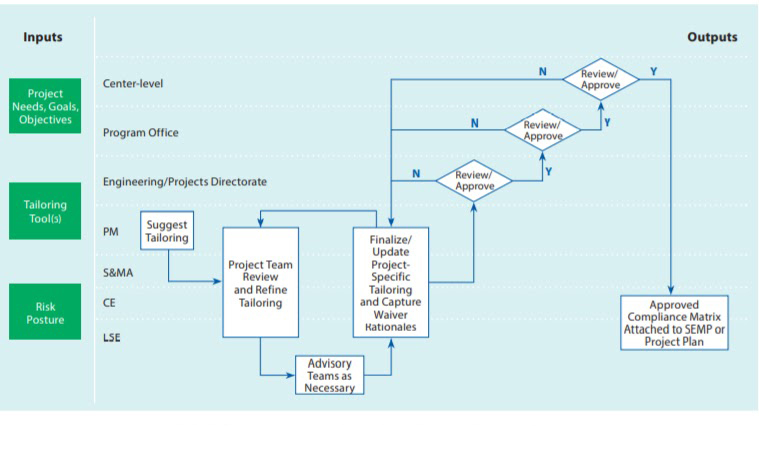
\includegraphics[width=0.8\textwidth]{figures/3.1.jpg}
    \caption{\href{https://www.nasa.gov/wp-content/uploads/2018/09/nasa_systems_engineering_handbook_0.pdf?emrc=4096b9}{Processus de personnalisation des produits de vol spatial national.}}
    \label{fig:communication2}
\end{figure}
Les caractéristiques d’un programme ou d’un projet spatial peuvent être décomposées selon les paramètres suivants :  
\begin{itemize}
    \item \textbf{Type de mission} : Par exemple, les exigences pour une mission habitée sont beaucoup plus strictes que celles d’une petite mission robotique.  
    \item \textbf{Criticité de la mission} dans la réalisation du Plan stratégique de l’Agence : Les missions critiques qui doivent absolument réussir peuvent ne pas être exemptées des exigences NPR (NASA Procedural Requirements).  
    \item \textbf{Niveau de risque acceptable} : Si l’Agence et le client acceptent un risque d’échec plus élevé, certaines exigences NPR peuvent être levées.  
    \item \textbf{Importance nationale} : Un projet ayant une grande importance nationale peut ne pas être exempté des exigences NPR.  
    \item \textbf{Complexité} : Les missions très complexes peuvent nécessiter davantage d’exigences NPR pour assurer la compatibilité des systèmes, tandis que les missions plus simples peuvent être soumises à une rigueur moindre.  
    \item \textbf{Durée de vie de la mission} : Les missions à long terme doivent se conformer plus strictement aux exigences NPR que les programmes/projets de courte durée.  
    \item \textbf{Coût de la mission} : Les missions plus coûteuses peuvent nécessiter une conformité plus stricte aux exigences NPR afin d’assurer un contrôle adéquat du programme/projet.  
    \item \textbf{Contraintes de lancdement} : Si de nombreuses contraintes de lancement existent, un projet peut devoir se conformer davantage aux exigences de l’Agence.  
\end{itemize}
\begin{figure}[H] % H force l'affichage ici
    \centering
    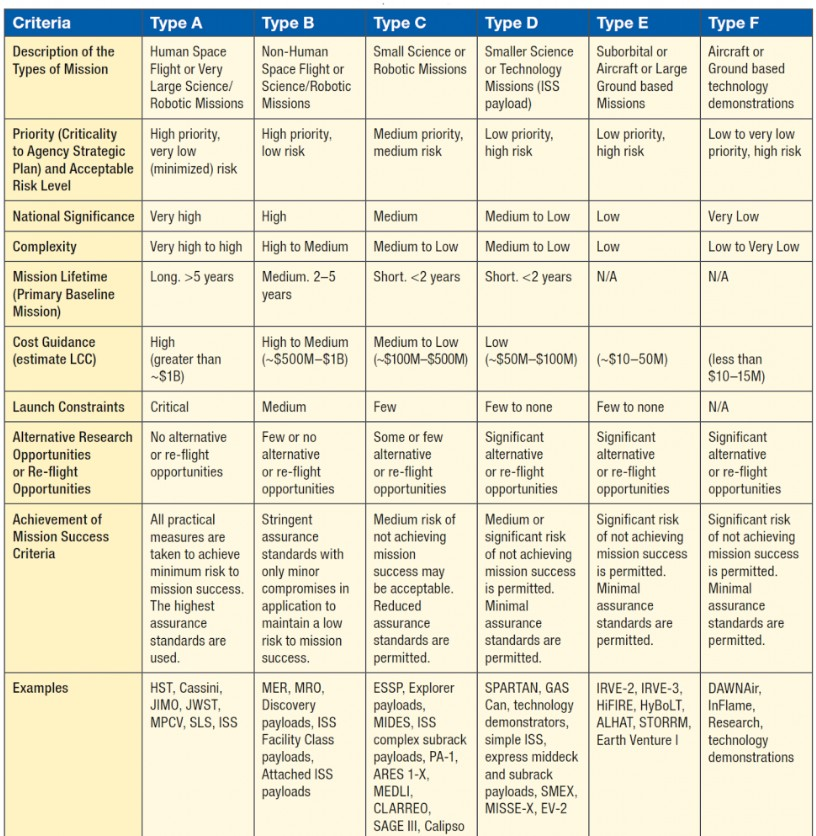
\includegraphics[width=0.8\textwidth]{figures/3.2.jpg}
    \caption{Example of program and project types. Image courtesy of NASA System Engineering Textbook.}
    \label{fig:communication2}
\end{figure}
\begin{itemize}
    \item Pour ce cours, nous nous concentrons sur des programmes similaires au Type D, où les programmes sont :
    \begin{itemize}
        \item de faible priorité,  
        \item à haut risque,  
        \item minimalement complexes,  
        \item de faible importance nationale,  
        \item avec de petits budgets,  
        \item des durées de mission courtes,  
        \item et de nombreuses opportunités alternatives ou de re-lancement.  
    \end{itemize}
    
    \item Les missions CubeSat se situent à l'extrême limite des missions de Type D :
    \begin{itemize}
        \item Les coûts des programmes dirigés par des étudiants dépassent rarement des dizaines de milliers de dollars américains.  
        \item Ces programmes sont principalement éducatifs (faible importance), avec peu ou pas d'exigence de succès.  
        \item Ils se terminent généralement en quelques années.  
    \end{itemize}
    
    \item Les CubeSats sont un excellent moyen de :
    \begin{itemize}
        \item démontrer des \href{https://www.nasa.gov/smallsat-institute/sst-soa}{technologies} de pointe à moindre coût,  
        \item lancer une multitude de satellites pour tester des concepts de détection distribuée,  
        \item offrir des missions innovantes.  
    \end{itemize}
    
    \item Pour les composants du bus spatial qui ne sont pas la charge utile, il existe de nombreuses pièces commerciales disponibles sur le marché (\href{http://www.cubesat.org/}{Commercial Off-The-Shelf, COTS}).  
    
    \item En ce qui concerne le financement :
    \begin{itemize}
        \item Le programme NASA CSLI est probablement la meilleure option pour envoyer votre CubeSat dans l’espace en tant qu’organisation étudiante.  
        \item Le manuel CSLI contient de nombreux conseils pour la rédaction des propositions, comme illustré dans la figure ci-dessus.  
        \item Vous pouvez également obtenir un financement potentiel pour l’achat de matériel ou le financement de la main-d’œuvre via le \href{https://www.nasa.gov/stem/spacegrant/home/Space_Grant_Consortium_Websites.html}{NASA Space Grant Consortium} de votre État.  
    \end{itemize}
\end{itemize}
\begin{itemize}
    \item Le financement participatif est également une option, comme pour les projets \href{https://www.planetary.org/sci-tech/lightsail}{LightSail} ou \href{https://www.kickstarter.com/projects/zacinaction/kicksat-your-personal-spacecraft-in-space}{KickSat}.  
    \item Un financement commercial via le capital-risque est possible si vous avez un modèle économique rentable, comme \href{https://spire.com/}{Spire}.  
\end{itemize}
\begin{figure}[H] % H force l'affichage ici
    \centering
    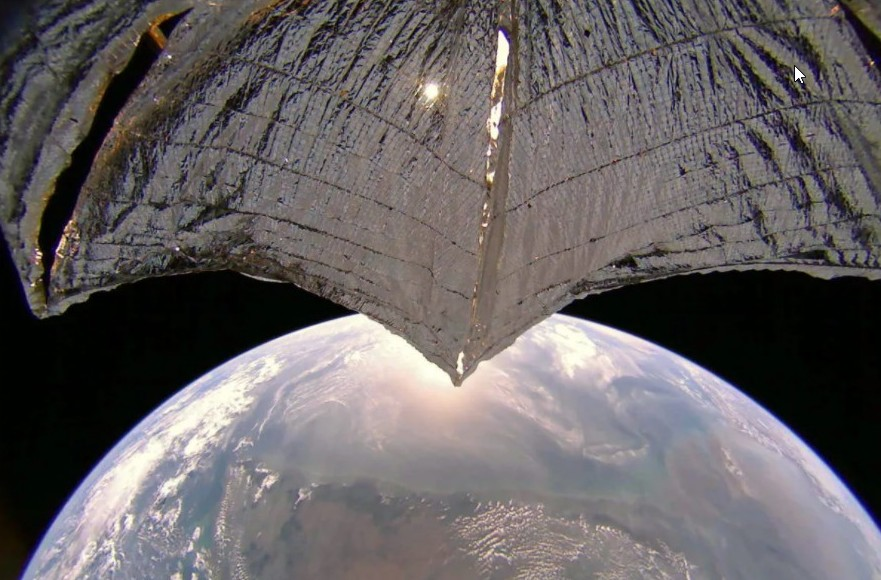
\includegraphics[width=0.8\textwidth]{figures/3.4.jpg}
    \caption{Light Sail 2 over India Light Sail 2 regularly transmits images from its onboard cameras. These images help engineers track the condition of the sail while providing stunning public outreach images. Image courtesy of The Planetary Society}
    \label{fig:communication2}
\end{figure}
\subsection{Processus de révision}
\begin{itemize}
    \item Au cours des différentes revues, trouvez une communauté capable de vous fournir un retour honnête sur votre capacité à respecter la conception de la mission et à gérer le coût et le budget.  
    \item Vous pouvez rejoindre une \href{http://cubesatquestions.slack.com/}{communauté CubeSat sur Slack}, participer aux forums Pressbooks ou solliciter des mentors académiques de votre université.  
    \item Il est essentiel d’avoir des examinateurs qui possèdent des connaissances et une expérience dans votre domaine de spécialisation (science, technologie et/ou éducation), qui peuvent évaluer la nécessité d’une opportunité de vol, qui ont une expertise en vol spatial et en engins spatiaux, mais aussi des compétences générales en développement matériel et en gestion de projet.  
    \item L’un des rôles des examinateurs est d’évaluer la capacité de votre équipe à livrer le satellite à temps et dans le respect du budget.  
    \item Assurez-vous d’inclure votre client dans ce panel d’examen.  
    \item Il est possible d’avoir plusieurs examinateurs afin de couvrir l’ensemble des compétences requises.  
\end{itemize}
\begin{figure}[H] % H force l'affichage ici
    \centering
    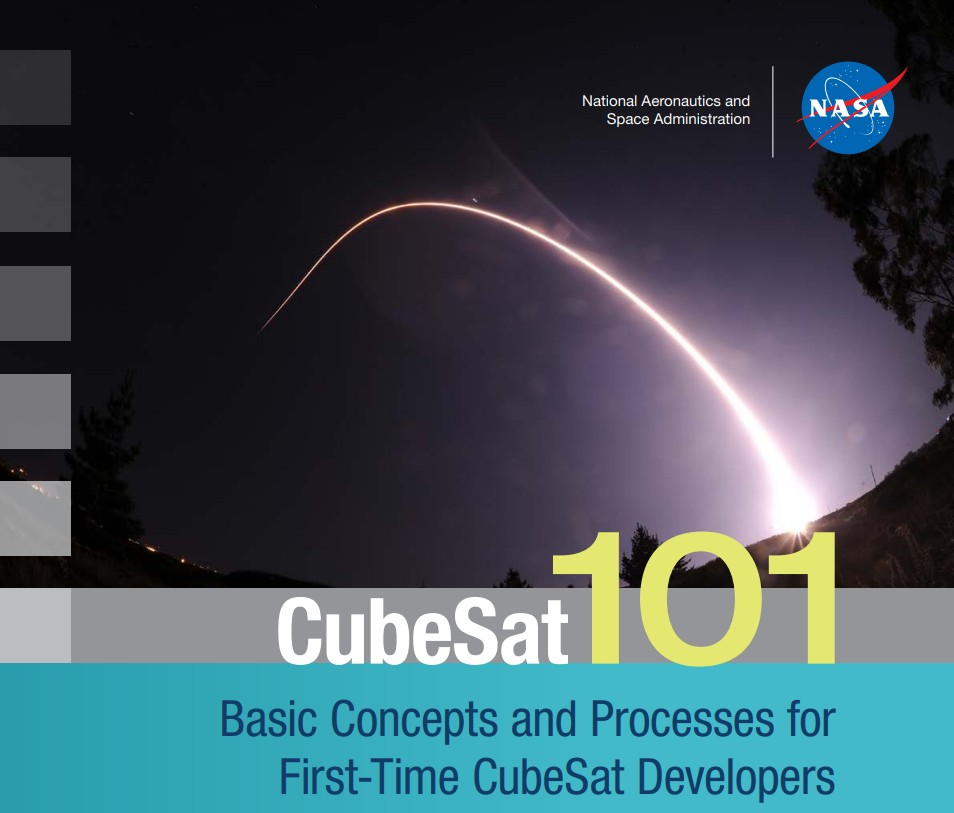
\includegraphics[width=0.8\textwidth]{figures/3.5.jpg}
    \caption{\href{https://www.nasa.gov/wp-content/uploads/2017/03/nasa_csli_cubesat_101_508.pdf}{CubeSat 101. Basic concepts and processes for first-time developers. Image courtesy of NASA.}}
    \label{fig:communication2}
\end{figure}
\subsection{Processus de conception}
\begin{itemize}
    \item Pendant le processus de conception, vous aurez besoin de divers logiciels qui peuvent vous faire gagner du temps et vous permettre d'obtenir de meilleurs résultats plutôt que de réinventer la roue.  
    \item Nous ne mentionnerons que des logiciels gratuits afin de réduire les barrières financières associées à ce projet.  
    \item La conception et l’analyse structurelles mécaniques peuvent être réalisées avec OnShape ou Autodesk Inventor.  
    \item La conception et la simulation des cartes électroniques peuvent être effectuées avec Eagle, KiCAD, \href{http://4pcb.com/}{PCB Artist} et PSpice.  
    \item L'analyse thermique peut être réalisée avec Thermal Desktop.  
    \item La conception et l’analyse d’orbite peuvent être effectuées avec STK.  
    \item Les logiciels de vol peuvent être développés à l’aide de la version open-source du CFS de la NASA, \href{https://github.com/OpenSatKit/OpenSatKit}{OpenSat Kit}.  
\end{itemize}

\textbf{Spécificité du kit Artemis}
\begin{itemize}
    \item Le Hawaii Space Flight Laboratory (HSFL) fournit sa propre suite logicielle appelée COSMOS, incluse avec votre kit.  
    \item Ce logiciel est conçu pour assister la conception de satellites et la planification des missions en intégrant divers outils de simulation, de test et d’opération.  
    \item Tout au long des modules de laboratoire et des tutoriels, COSMOS sera utilisé pour vous guider dans les activités essentielles de conception de satellites.  
    \item Des instructions détaillées étape par étape vous permettront d’apprendre les fonctionnalités et procédures logicielles pertinentes.  
    \item Cette approche structurée garantit une expérience pratique complète en matière de conception, de test et d’exploitation d’un système satellite.  
\end{itemize}
\subsection{Processus de développement}
\begin{itemize}
    \item Pendant le processus d’approvisionnement et de fabrication, vous devrez porter une attention particulière à la façon dont vous vous procurez vos matériaux ainsi qu’à l’équipement nécessaire pour rendre ce matériel apte au vol spatial.  
    \item Le kit Artemis CubeSat devrait être complet et prêt à être lancé tel quel. Si vous souhaitez démontrer une mission entièrement centrée sur le logiciel, vous pouvez ignorer cette section.  
    \item Cependant, si vous souhaitez modifier des composants ou repartir de zéro, sachez que les aspects les plus importants lors du choix du matériel auprès de fournisseurs spécifiques sont :  
    \begin{itemize}
        \item l’aptitude au vol spatial,  
        \item le contrôle des exportations.  
    \end{itemize}
\end{itemize}
\textbf{Composants CubeSat et personnalisation}
\begin{itemize}
    \item Avec la multiplication des \href{http://www.cubesat.org/}{fournisseurs de CubeSat}, la variété des composants commerciaux standard (COTS) permet une plus grande personnalisation et une meilleure adéquation aux exigences techniques.  
    \item En dehors des exigences techniques, les caractéristiques des composants incluent l’héritage spatial, qui est lié au coût, à la main-d'œuvre et aux risques.  
    \item En général, les composants ayant été rigoureusement testés et ayant déjà volé dans l’espace (TRL 9) réduisent le besoin de tests rigoureux et diminuent le risque opérationnel de la mission.  
    \item L’inconvénient des composants qualifiés pour l’espace est leur coût élevé, qui reflète les dépenses liées au développement, aux tests et à la validation en conditions spatiales.  
    \item Plusieurs raisons peuvent justifier l’achat d’un composant COTS auprès d’un fournisseur électronique et la réalisation des tests en interne :  
    \begin{itemize}
        \item Le coût du composant qualifié pour l’espace est trop élevé.  
        \item Le composant non qualifié pour l’espace est mieux adapté aux exigences.  
        \item L’objectif de la mission est de développer un héritage spatial pour ce composant.  
    \end{itemize}
    \item L’inconvénient de faire mûrir la technologie en interne est le coût supplémentaire en main-d'œuvre et en équipement de test, ainsi que le risque accru à gérer.  
    \item Pour les grands projets, la mentalité consiste à minimiser les risques autant que possible, en utilisant souvent des composants qualifiés pour l’espace, ce qui peut conduire à l’utilisation de technologies obsolètes.  
\end{itemize}
\textbf{Spécificités du kit Artemis}
\begin{itemize}
    \item La mentalité des petits projets, comme les CubeSats, est d’accepter et de tolérer un niveau de risque plus élevé, ce qui a guidé l’équipe de conception du kit Artemis CubeSat.  
    \item HSFL dispose de toutes les installations de test nécessaires (table de vibration, chambres à vide thermique, banc de test dynamique et salle blanche) pour réaliser les tests de vérification du kit Artemis CubeSat.  
    \item Aucun des composants n’est qualifié pour l’espace, ce qui nous permet de proposer le kit à un coût très bas. Cependant, tous les composants ont été rigoureusement testés pour garantir leur bon fonctionnement théorique en environnement spatial.  
    \item Si vous ajoutez une charge utile ou modifiez l’un des composants, vous devrez suivre des procédures de test similaires à celles que nous détaillerons dans les chapitres suivants (HSFL est disponible pour fournir un support).  
\end{itemize}

\textbf{Contrôles à l’exportation des États-Unis}

\begin{itemize}
    \item Les réglementations américaines sur l’exportation pour l’industrie spatiale commerciale influencent la composition des équipes en raison de leur impact sur la capacité des membres de différentes nationalités à travailler sur des technologies contrôlées.  
    \item « Le système de contrôle des exportations des États-Unis est conçu pour empêcher la diffusion de technologies sensibles vers des acteurs étrangers pouvant menacer les intérêts américains, tout en permettant aux entreprises américaines de mener des activités commerciales légitimes. Les technologies contrôlées incluent les articles de défense (ex. : missiles), les services de défense (ex. : intégration d’un engin spatial sur un lanceur) et les articles à double usage (ex. : engins spatiaux commerciaux et composants). »  
    \item Il existe deux ensembles de réglementations :  
    \begin{itemize}
        \item \textbf{International Traffic in Arms Regulations (ITAR)} : contrôle les articles, informations ou activités pouvant être utilisés à des fins militaires étrangères, qu’il s’agisse de produits (articles de défense) ou d’assistance (services de défense).  
        \item \textbf{Export Administration Regulations (EAR)} : contrôle les articles et technologies considérés comme à « double usage », c’est-à-dire utilisables à la fois pour des applications commerciales et militaires. La majorité des engins spatiaux commerciaux et de leurs composants relèvent de la juridiction de l’EAR.  
    \end{itemize}
\end{itemize}

\textbf{Spécificités du kit Artemis}

\begin{itemize}
    \item Nous consacrerons une section aux réglementations ITAR et EAR, mais pour le kit Artemis CubeSat, aucun composant n’est soumis à ces réglementations, ce qui signifie que toute personne peut travailler avec les technologies du kit.  
\end{itemize}

%\section{Composantes de la mission}
\href{https://youtu.be/oWrt5QuPc0M}{Visualiser la Video}
\subsection{Objectif du processus d'ingénierie de mission spatiale}
L'objectif global du processus d'ingénierie de mission spatiale (présenté dans le chapitre précédent) est de définir un concept de mission de manière à inclure les composants suivants :
\begin{enumerate}
    \item Sujet  
    \item Charge utile  
    \item Bus spatial  
    \item Station au sol  
    \item Opérations de mission  
    \item Architecture de commande, de contrôle et de communication  
    \item Orbite  
    \item Segment de lancement  
\end{enumerate}
Ce cours se concentrera principalement sur la conception du bus spatial, mais abordera brièvement l'influence des autres composants sur sa conception.
\subsection{Sujet et Charge Utile}
La mission est centrée sur le sujet, qui comprend les phénomènes physiques ou les objets que le satellite doit observer, découvrir ou manipuler. Ces sujets peuvent inclure :
\begin{itemize}
    \item Les ondes gravitationnelles \textit{(GRACE)}
    \item Les fréquences d'Internet à large bande \textit{(Starlink)}
    \item Les astéroïdes \textit{(OSIRIS-REx)}
    \item Les neutrons \textit{(Neutron-1)}
\end{itemize}
Nous supposerons que vous avez abordé cette thématique en dehors de ce cours, par exemple dans \textit{EPET 301: Space Science Instrumentation}, ou avec vos collègues scientifiques et technologues qui sont vos clients. Vous pouvez également trouver des missions scientifiques ou technologiques intéressantes dans les enquêtes décennales de la NASA, ses plans stratégiques, ses feuilles de route et son rapport de taxonomie.

Le sujet influence les exigences orbitales si le satellite doit être proche de la source du sujet pour le détecter (comme pour \textit{OSIRIS-REx, GRACE} et \textit{Neutron-1}).
\subsection{Architecture de Commande, Contrôle et Communication}
\begin{itemize}
    \item L’architecture de commande, contrôle et communication est l’interface entre les opérations de mission, la station au sol et le satellite.
    \item Elle inclut le lien de télécommunication entre le satellite et la station au sol, ainsi que les connexions filaires ou sans fil entre la station au sol et le centre de contrôle de mission.
    \item Idéalement, le chemin du signal est aussi ininterrompu que possible pour permettre une transmission d’informations en temps réel, essentielle pour les missions à haute priorité.
    \item Pour les missions à faible priorité, les communications peuvent être retardées.
    \item Par exemple, il est possible de s’appuyer sur des opérateurs radioamateurs pour capter et transmettre les signaux, bien qu’il n’y ait aucune garantie qu’ils soient à l’écoute ou qu’ils transmettent les paquets reçus.
\end{itemize}

La charge utile est le matériel ou le logiciel qui détecte, mesure ou interagit avec le sujet. Si le sujet est le \textit{quoi}, la charge utile est le \textit{comment}. Il peut exister différents niveaux de charge utile si l'on élargit le périmètre du système. Par exemple :
\begin{itemize}
    \item Pour la mission \textit{Neutron-1}, la charge utile est un détecteur de neutrons.
    \item Si l'on considère la fusée qui lance \textit{Neutron-1} dans l'espace, la charge utile de la fusée est le satellite entier \textit{Neutron-1}.
\end{itemize}

Nous nous concentrerons strictement sur la charge utile intégrée au bus spatial, auquel une section entière sera dédiée, car le sujet et la charge utile influencent directement la conception du bus spatial.

\textbf{Kit Artemis CubeSat}
\begin{itemize}
    \item Une caméra opérant dans le spectre infrarouge et visible est incluse afin de favoriser les missions d'observation de la Terre et de la Lune.  
    \item Possibilité de retirer la caméra et d'utiliser un quart du volume du CubeSat pour une charge utile personnalisée.  
    \item Conception du bus spatial adaptable à une variété de :
    \begin{itemize}
        \item Connecteurs électriques  
        \item Tensions acceptables  
        \item Besoins en énergie  
    \end{itemize}
\end{itemize}
\subsection{Segment Sol}
Le segment sol comprend tous les composants restant au sol :  
\begin{itemize}  
    \item Station terrestre  
    \item Opérations de mission  
    \item Architecture de commande, de contrôle et de communication  
\end{itemize}
\begin{figure}[H] % H force l'affichage ici
    \centering
    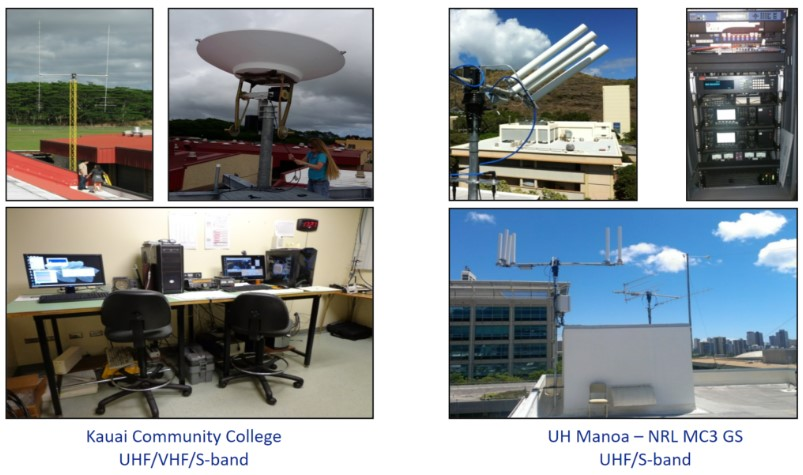
\includegraphics[width=0.8\textwidth]{figures/3.7.jpg}
    \caption{\href{https://www.hsfl.hawaii.edu/ground-stations/}{Examples of ground stations. Image Source: HSFL}}
    \label{fig:communication2}
\end{figure}
\textbf{Station Sol}

\begin{itemize}
    \item Une station sol est une \textit{« station radio terrestre con\^cue pour la t\'el\'ecommunication extraplan\'etaire avec un vaisseau spatial »}.
    \item R\^oles principaux :
    \begin{itemize}
        \item Communiquer et contr\^oler les engins spatiaux.  
        \item Recevoir des signaux faibles envoy\'es par le vaisseau spatial.  
        \item Transmettre des signaux puissants vers le vaisseau spatial.  
    \end{itemize}
    \item Caract\'eristiques des grandes stations sol :
    \begin{itemize}
        \item Antenne parabolique offrant une forte directivit\'e.  
        \item D\'etection de signaux radio sensibles provenant de sources astronomiques.  
        \item Exemples : \textbf{Deep Space Network} de la NASA.  
    \end{itemize}
    \item Les d\'ecouvertes astronomiques modernes utilisent des antennes plus grandes que celles n\'ecessaires aux communications spatiales.  
\end{itemize}
\begin{figure}[H] % H force l'affichage ici
    \centering
    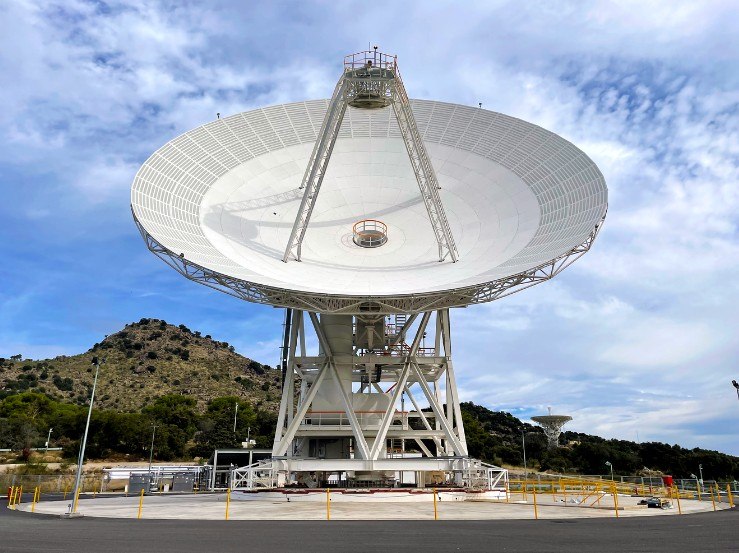
\includegraphics[width=0.8\textwidth]{figures/3.8-1.jpg}
    \caption{Example of a large dish in NASA’s Deep Space Network. Image courtesy of NASA.}
    \label{fig:communication2}
\end{figure}
\begin{figure}[H] % H force l'affichage ici
    \centering
    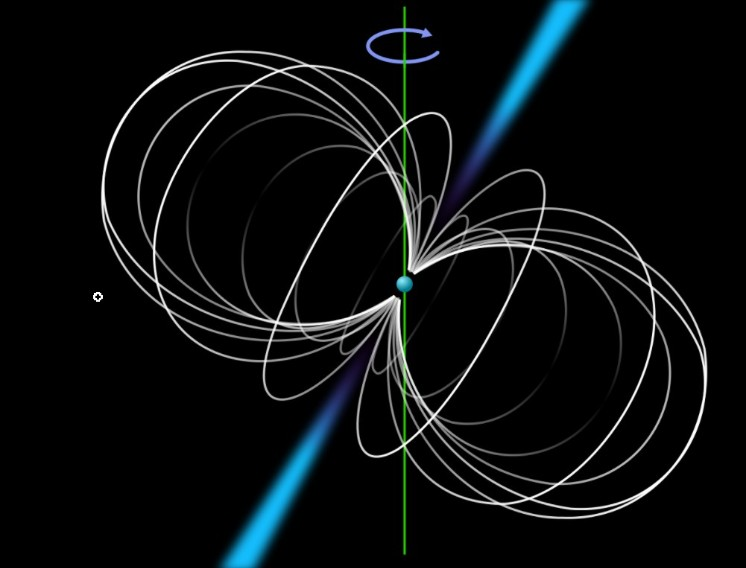
\includegraphics[width=0.8\textwidth]{figures/3.9.jpg}
    \caption{Example of an astronomical radio source. This is a schematic view of a pulsar. The sphere in the middle represents the neutron star, the curves indicate the magnetic field lines, the protruding cones represent the emission beams and the green line represents the axis on which the star rotates. Image by Roy Smits.}
    \label{fig:communication2}
\end{figure}
\textbf{Stations sol de petite taille}

\begin{itemize}
    \item Elles utilisent g\'en\'eralement un r\'eseau d'antennes dip\^oles, la classe d'antennes la plus courante dans la vie quotidienne.
    \item Caract\'eristiques :
    \begin{itemize}
        \item Omnidirectionnelles.  
        \item Construction simplifi\'ee.  
        \item Compr\'ehension th\'eorique plus accessible, ce qui les rend adapt\'ees aux \'equipes universitaires.  
    \end{itemize}
    \item Suivi des satellites :
    \begin{itemize}
        \item Les antennes, qu'elles soient de petite ou grande taille, peuvent \^etre fixes ou orientables pour suivre un satellite.
        \item Les grandes antennes directionnelles suivent rarement les signaux dynamiquement en raison de la complexit\'e des syst\`emes de support pour des masses importantes.
    \end{itemize}
    \item La construction des stations sol est hors du champ de ce cours, mais plusieurs options sont disponibles :
    \begin{itemize}
        \item Contacter \textbf{HSFL} pour un support missionnel.
        \item Planifier un acc\`es via les services \textbf{AWS Ground Station}.
        \item Participer \`a \textbf{SatNOGS}, un r\'eseau mondial open-source de stations sol.  
    \end{itemize}
\end{itemize}
\begin{figure}[H] % H force l'affichage ici
    \centering
    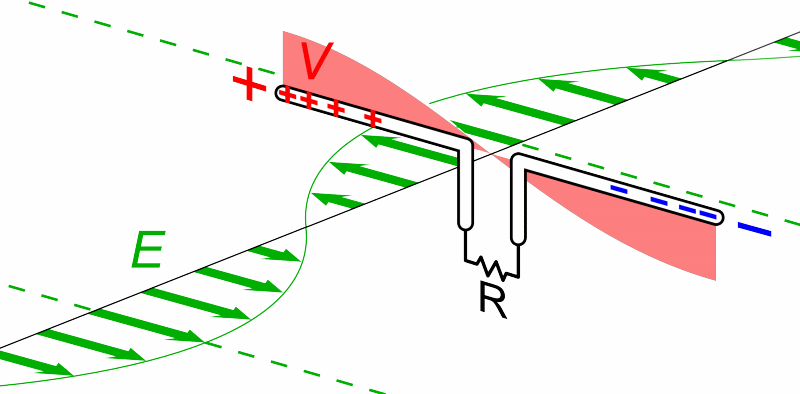
\includegraphics[width=0.8\textwidth]{Dipole_receiving_antenna_animation_6_800x394x150ms-2.png}
    \caption{Animated diagram of a half-wave dipole antenna receiving a radio wave. Image by Chet Vorno.}
    \label{fig:communication2}
\end{figure}

\subsection{Op\'erations de mission}
\begin{itemize}
    \item L'\'equipe des op\'erations de mission peut \^etre compos\'ee de sp\'ecialistes distincts dans un grand programme, comme les op\'erateurs du rover \textbf{Curiosity} de la NASA qui ont d\^u suivre une formation sp\'ecifique, ou bien des membres de l'\'equipe de conception du satellite pour les petits projets. 

    \item Si vous \^etes \'etudiant dans une petite \'equipe, vous serez tr\`es probablement l'un des op\'erateurs de mission ; et qui mieux que l'un des ing\'enieurs ayant con\c{c}u le satellite pour l'op\'erer ? Vous aurez l'avantage unique de conna\^itre pr\'ecis\'ement les capacit\'es du vaisseau spatial sans avoir besoin de consulter un ing\'enieur ext\'erieur, car cet ing\'enieur, c'est vous !  

    \item Le logiciel d'op\'erations de mission permet aux op\'erateurs de surveiller l'\'etat de sant\'e du vaisseau spatial ainsi que les param\`etres pertinents de la mission, tout en envoyant des commandes depuis un ordinateur. La NASA a d\'evelopp\'e \textbf{Open MCT}, un cadre de visualisation de donn\'ees de mission de nouvelle g\'en\'eration, bas\'e sur le Web, et con\c{c}u pour les environnements de bureau et mobiles.
\end{itemize}
\textbf{Sp\'ecificit\'es du kit Artemis}
\begin{itemize}
    \item Le kit Artemis CubeSat est fourni avec \textbf{COSMOS}, un package logiciel permettant le d\'eveloppement de logiciels de vol et offrant une interface pour les op\'erations de mission.
\end{itemize}
\begin{figure}[H] % H force l'affichage ici
    \centering
    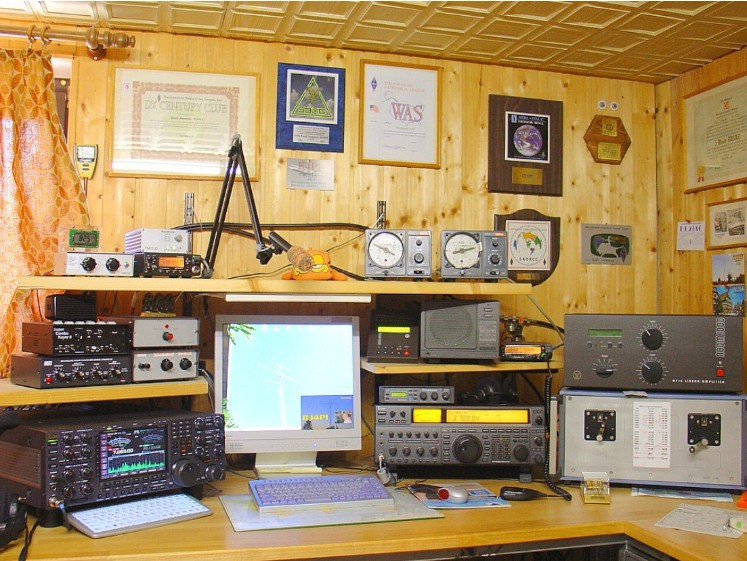
\includegraphics[width=0.8\textwidth]{figures/3.11.jpg}
    \caption{Example of amateur radio. Image by Emil Neuerer.}
    \label{fig:communication2}
\end{figure}
\textbf{Spécificité du Kit Artemis}
\begin{itemize}
    \item Pour le kit Artemis CubeSat, nous recommandons de collaborer avec HSFL.
    \item La conception du satellite intègre les stations au sol de HSFL, le logiciel d'opérations de mission et les interfaces correspondantes.
\end{itemize}

\textbf{Décision Critique sur l'Architecture de Communication}
\begin{itemize}
    \item Le choix de la \textbf{fréquence de communication} et l'obtention de la licence RF correspondante sont des étapes essentielles [CSLI Chapitre 9].
    \item Le kit \textbf{Artemis CubeSat} ne peut obtenir qu'une \textbf{licence radioamateur ou expérimentale}.
    \item Nous vous accompagnerons dans la documentation nécessaire pour l'obtention de la \textbf{licence FCC} [FCC Guidance et Spectrum Guidance].
    \item Ce processus est \textbf{complexe et soumis à des goulets d'étranglement}, mais des efforts sont en cours pour le simplifier.
    \item Les autorités gouvernementales travaillent à une simplification \textbf{du haut vers le bas}, tandis que nous cherchons à vous former \textbf{du bas vers le haut}.
\end{itemize}
\begin{figure}[H] % H force l'affichage ici
    \centering
    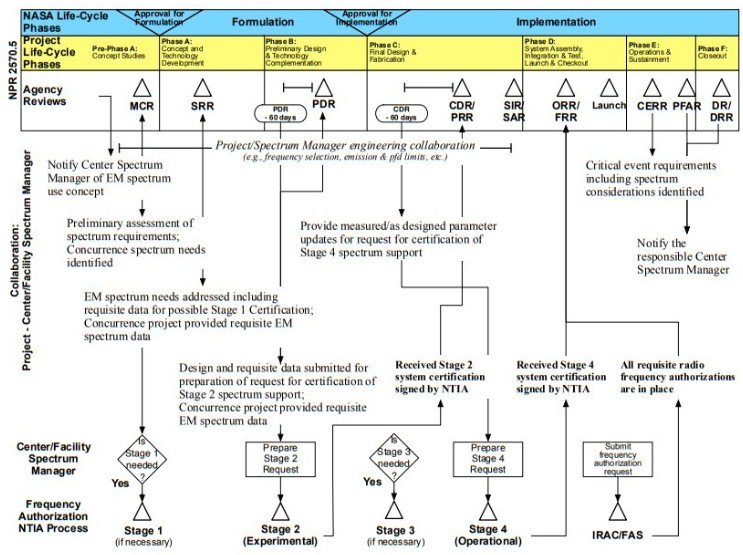
\includegraphics[width=0.8\textwidth]{figures/3.13.jpg}
    \caption{Spectrum certification process. Image courtesy of NASA.}
    \label{fig:communication2}
\end{figure}

\section*{Orbite et Lancement}

L'orbite correspond à la trajectoire du satellite au cours de sa mission par rapport aux corps planétaires et aux références astronomiques. Une section dédiée décrira en détail les différentes orbites et l’environnement spatial associé. Ce paragraphe offre une vue d’ensemble à un niveau plus global.

\begin{itemize}
    \item L’\textbf{orbite} détermine l’environnement spatial dans lequel le satellite doit évoluer ainsi que le lanceur avec lequel il doit être compatible.
    \item Les \textbf{caractéristiques orbitales} influencent les phénomènes physiques dominants dans cet environnement, imposant des exigences techniques spécifiques aux sous-systèmes du satellite pour atteindre l’objectif de la mission.
    \item L’\textbf{environnement spatial} peut également impacter les opérations de mission, en raison des délais de communication ou des interruptions de signal (\textit{blackouts}).
    \item La \textbf{distance} à parcourir ou le \textbf{delta-V} requis pour atteindre l’orbite souhaitée influence la taille du lanceur.
    \item Le lanceur impose des \textbf{contraintes de volume} en raison des dimensions de sa coiffe, dans laquelle le satellite doit s’intégrer.
\end{itemize}
\begin{figure}[H] % H force l'affichage ici
    \centering
    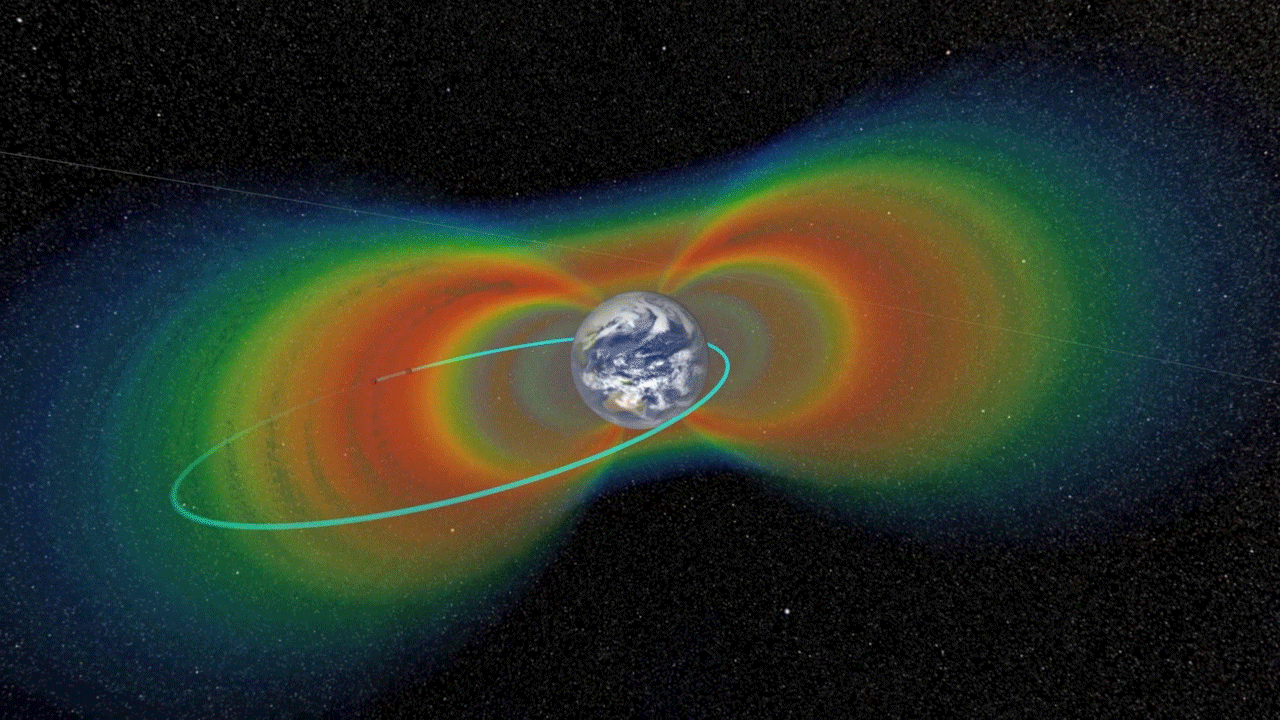
\includegraphics[width=0.8\textwidth]{figures/nasasvanalle.png}
    \caption{Example of an orbital path of a spacecraft. Image courtesy of Physics.org}
    \label{fig:communication2}
\end{figure}
\textbf{Spécificité du Kit Artemis}

\begin{itemize}
    \item Le matériel fourni avec le \textbf{kit Artemis CubeSat} est conçu pour fonctionner en \textbf{orbite basse terrestre} (LEO).
    \item Plus précisément, il est optimisé pour une \textbf{orbite similaire à celle de l’ISS}, car de nombreux CubeSats sont déployés depuis la Station Spatiale Internationale.
\end{itemize}
\textbf{Déploiement des CubeSats 1U}

\begin{itemize}
    \item Les \textbf{CubeSats 1U} sont généralement \textbf{intégrés dans des déployeurs} au sol.
    \item Ils sont ensuite \textbf{transportés vers l’ISS} dans un \textbf{vaisseau cargo pressurisé} (par exemple, \textbf{SpaceX Dragon} ou \textbf{Orbital ATK Cygnus}).
    \item Une fois à bord de l’ISS, ils sont \textbf{manipulés manuellement} par les astronautes.
    \item Les CubeSats sont habituellement \textbf{déployés de l’ISS 1 à 3 mois après leur arrivée} [CSLI Chapitre 3.5].
\end{itemize}

\textbf{Spécificités du Kit Artemis}
\begin{itemize}
    \item Si le \textbf{CubeSat Artemis} n’est pas stocké en douceur (\textit{softly stowed}), 
    \item Le kit a été testé selon les \textbf{normes NASA CSLI} pour survivre au \textbf{ridesharing} en tant que \textbf{charge utile auxiliaire} montée directement sur les lanceurs [NASA GEVS].
\end{itemize}

\begin{itemize}
    \item Si vous choisissez de lancer en dehors de l'écosystème \textbf{CSLI}, comme \textbf{UNP},  
    \item Vous pouvez trouver d'autres \textbf{fournisseurs de lancement} avec leurs propres normes de tests environnementaux.
    \item Idéalement, ces normes sont \textbf{moins rigoureuses} que celles du \textbf{CSLI}, 
    \item Ce qui éviterait de refaire tous les tests environnementaux que nous avons déjà réalisés pour vous.
\end{itemize}
\begin{figure}[H] % H force l'affichage ici
    \centering
    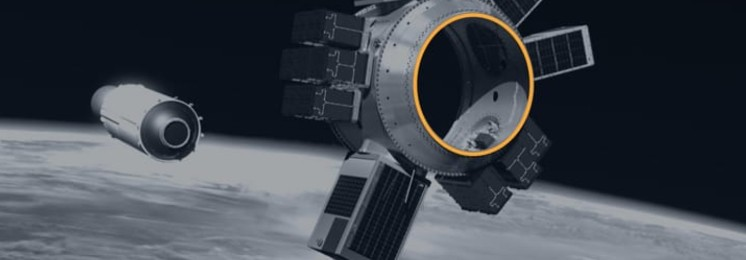
\includegraphics[width=0.8\textwidth]{3.14.jpg}
    \caption\href{https://blog.satsearch.co/2019-12-04-find-a-launch-option-for-your-cubesat-or-small-satellite-an-overview-of-launch-service-providers}{Select a launch provider for your CubeSat. Image courtesy of Spaceflight Industries.}
    \label{fig:communication2}
\end{figure}
\subsection{Bus Spatial}
\begin{itemize}
    \item Lors de la conception préliminaire, il est recommandé d'allouer des budgets de \textbf{masse} et de \textbf{puissance} pour un satellite sans propulsion.
    \item Un \textbf{ingénieur systèmes} est généralement chargé du suivi de ces budgets, ainsi que d'autres paramètres tels que :
    \begin{itemize}
        \item L'alignement et le pointage pour l'\textbf{ADCS}.
        \item Le \textbf{propulseur}, si le satellite est propulsif.
        \item La \textbf{liaison montante et descendante} pour les communications.
        \item L'utilisation des données pour le \textbf{traitement des commandes et des données}.
    \end{itemize}
    \item Ces budgets seront détaillés dans les sections consacrées aux sous-systèmes correspondants.
\end{itemize}

\begin{table}[h]
    \centering
    \begin{tabular}{|l|c|c|c|}
        \hline
        \textbf{Sous-système} & \textbf{SMAD sugg} & \textbf{Hermes CubeSat} & \textbf{Artemis CubeSat} \\
        \hline
        Charge utile & 41\% & Allocated in T\&C & 2\% \\
        \hline
        Structure et Mécanismes & 20\% & 32.3\% & 20\% \\
        \hline
        Contrôle thermique & 2\% & 0\% & 0\% \\
        \hline
        Puissance (y compris harnais) & 19\% & 13.5\% & 48\% \\
        \hline
        Télémétrie et Contrôle & 2\% & 22.5\% & 5\% \\
        \hline
        Commande et Traitement des Données & 5\% & 3.6\% & 18\% \\
        \hline
        Détermination et Contrôle d'Attitude & 8\% & 2.4\% & 8\% \\
        \hline
        Autres (équilibrage + lancement) & 3\% & 25.7\% & 0\% \\
        \hline
        \textbf{Total} & 100\% & 100\% & 100\% \\
        \hline
    \end{tabular}
    \caption{Répartition de la masse sèche des sous-systèmes des CubeSats}
    \label{tab:subsystem_mass}
\end{table}





%\section{Conception de la charge utile}
\href{https://youtu.be/uHOsxEK5CUA}{Visualiser la Video}


\textbf{Sujet et Charge Utile}

\begin{itemize}
    \item Le \textbf{sujet} et la \textbf{charge utile} sont les principaux moteurs de conception, car ils justifient l'existence de la mission.
    \item Le sujet détermine :
    \begin{itemize}
        \item L'\textbf{emplacement} ou l'\textbf{orbite} que le vaisseau spatial doit atteindre.
        \item La \textbf{charge utile} à intégrer.
        \item Toutes les \textbf{exigences de conception} qui influencent la conception du bus spatial.
    \end{itemize}
    \item Les classifications des charges utiles incluent :
    \begin{itemize}
        \item \textbf{Observation}.
        \item \textbf{Communications ou navigation}.
        \item \textbf{In situ}.
        \item \textbf{Action à distance}.
        \item \textbf{Vols spatiaux habités}.
    \end{itemize}
    \item La majorité des charges utiles des \textbf{CubeSats} concernent :
    \begin{itemize}
        \item L'\textbf{observation de la Terre}.
        \item La \textbf{communication}.
        \item La \textbf{navigation}.
        \item La \textbf{science et la technologie}.
    \end{itemize}
    \item Les charges utiles des vols spatiaux habités et celles d'\textbf{action à distance} sont rarement utilisées sur les CubeSats.
    \item Les charges utiles d'\textbf{observation} sont principalement utilisées pour :
    \begin{itemize}
        \item L'étude de l'\textbf{espace lointain} (\textit{exoplanètes, phénomènes astronomiques, effets du soleil sur la météo spatiale}).
        \item L'étude de la \textbf{Terre} (\textit{climat, surveillance, cartographie de la surface terrestre, plans d'eau}).
    \end{itemize}
    \item Ces charges utiles fonctionnent dans différentes \textbf{bandes de longueurs d'onde}.
\end{itemize}

\begin{figure}[H] % H force l'affichage ici
    \centering
    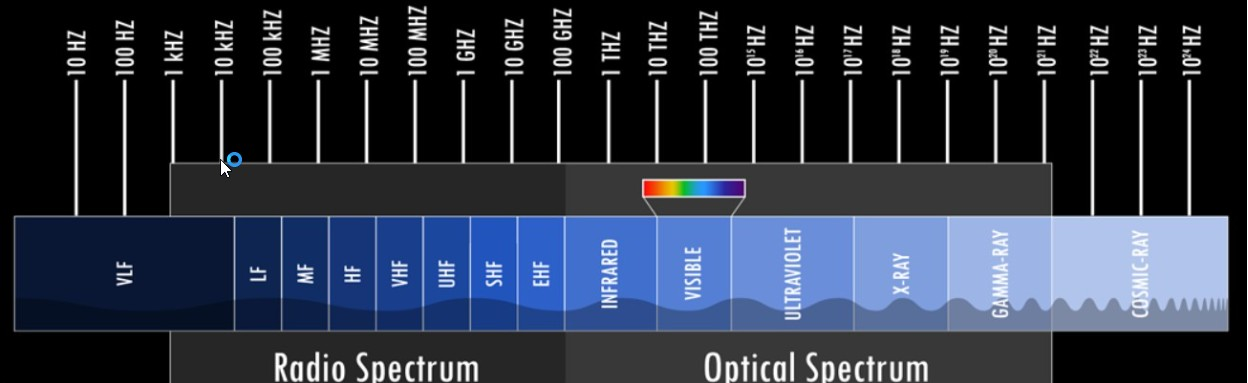
\includegraphics[width=0.8\textwidth]{figures/3.15.jpg}
    \caption{NASA electromagnetic spectrum mapping to space phenomena. Image courtesy of NASA.}
    \label{fig:communication2}
\end{figure}
\textbf{Types de Charges Utiles de Communication et Navigation}
\begin{itemize}
    \item Les charges utiles de \textbf{communication} peuvent être classées en :
    \begin{itemize}
        \item \textbf{Systèmes unidirectionnels} : recueillent des informations sans transmission active.  
        \item \textbf{Systèmes bidirectionnels} : recueillent et transmettent des informations.  
    \end{itemize}
    \item Les charges utiles de \textbf{navigation} suivent et transmettent des informations de position, comme :
    \begin{itemize}
        \item Le \textbf{système de positionnement global} (\textbf{GPS}).  
        \item Les plateformes de \textbf{radio définie par logiciel} (\textbf{SDR}).  
    \end{itemize}
    \item Les charges utiles \textbf{in-situ} mesurent directement les signaux de l’environnement qui ne peuvent pas être détectés à distance, tels que :
    \begin{itemize}
        \item Le \textbf{champ magnétique}.  
        \item La \textbf{gravité}.  
        \item La \textbf{collecte d’échantillons}.  
    \end{itemize}
\end{itemize}
\textbf{Spécificités du Kit Artemis}

\begin{itemize}
    \item Nous nous concentrerons sur les \textbf{charges utiles d'observation}, car le kit Artemis CubeSat est équipé d'une \textbf{caméra visible-IR}.  
    \item L'équipe \textbf{Ke Ao} de l'\textbf{UH Manoa} souhaite prendre une \textbf{photo d’Hawaï} depuis l'orbite terrestre basse et la transmettre aux opérateurs de mission.  
    \item La charge utile est une \textbf{caméra visible} basée sur un \textbf{Raspberry Pi}.  
\end{itemize}
\textbf{Contraintes de la Charge Utile}

Avant de concevoir le sous-système du bus spatial en fonction de la charge utile, il est essentiel d'examiner les contraintes liées à la conception de la charge utile. Il existe quatre types de contraintes :

\begin{itemize}
    \item \textbf{Contraintes fondamentales} :  
    \begin{itemize}
        \item Limite de diffraction.  
        \item Bruit photonique.  
        \item Limite de Nyquist.  
        \item Ces limites sont imposées par les lois de la physique et restreignent l'observation, rendant certaines missions impossibles, même avec des avancées technologiques.  
    \end{itemize}

    \item \textbf{Contraintes technologiques} :  
    \begin{itemize}
        \item Limitations des détecteurs de pointe (taille et performances).  
        \item Forme, précision, fabrication et alignement optiques.  
        \item Vitesse de traitement des données.  
        \item Même en dehors des limites théoriques, les détecteurs et optiques fabriqués auront des performances suboptimales.  
    \end{itemize}

    \item \textbf{Contraintes de mission} :  
    \begin{itemize}
        \item Contraintes de taille, de poids et de puissance (\textbf{SWaP}) dues à la conception du vaisseau spatial et au lanceur sélectionné.  
        \item Certaines charges utiles ne peuvent pas être miniaturisées davantage sans compromettre la performance de la mission.  
    \end{itemize}

    \item \textbf{Contraintes programmatiques} :  
    \begin{itemize}
        \item Coût.  
        \item Planning et délais.  
        \item Risques et exigences réglementaires.  
        \item Ces contraintes peuvent empêcher une mission réalisable sur le plan scientifique et technologique d’être menée à bien.  
    \end{itemize}
\end{itemize}

Cette séquence de contraintes évolue du niveau scientifique le plus élevé jusqu'aux réalités physiques et sociétales des missions spatiales.

\textbf{Spécificités du Kit Artemis}
\begin{itemize}
    \item Pour le projet \textbf{Ke Ao}, la charge utile n'est pas une technologie de pointe passée.  
    \item La caméra \textbf{Raspberry Pi} est une technologie éprouvée.  
    \item Ses caractéristiques physiques sont bien adaptées à une mission \textbf{CubeSat 1U}.  
    \item Les contraintes programmatiques sont relativement \textbf{flexibles}, car il s'agit d'un projet \textbf{intégré verticalement} dans un environnement universitaire.  
\end{itemize}
\begin{figure}[H]
    \centering
    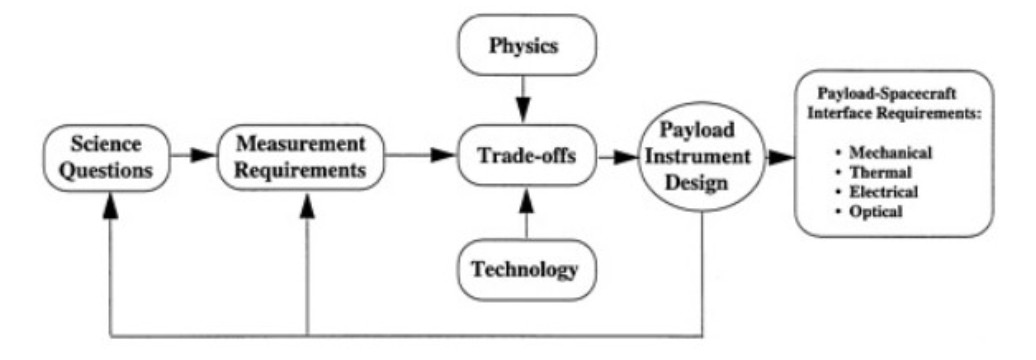
\includegraphics[width=0.8\textwidth]{figures/3.16.jpg}
    \caption{\protect\href{https://nap.nationalacademies.org/read/9819/chapter/5\#23}
    {Le processus de conception de la charge utile génère des exigences pour son intégration. Image courtoisie de NASA et NAP.}}
    \label{fig:communication2}
\end{figure}
\textbf{Définition de l'Architecture de Mission}

\begin{itemize}
    \item Une fois une \textbf{charge utile} identifiée et validée en respectant toutes les contraintes, la conception de l'architecture de mission peut commencer.
    \item Nous avons abordé les solutions pour les différents \textbf{composants de la mission}.
    \item Concernant le \textbf{concept des opérations}, nous nous concentrerons sur :
    \begin{itemize}
        \item La \textbf{durée de vie de la mission}.  
        \item La \textbf{séquence des événements} après l'arrivée du satellite dans l'espace.  
    \end{itemize}
\end{itemize}
\textbf{Spécificités du Kit Artemis}

\begin{itemize}
    \item Le \textbf{kit Artemis CubeSat} n'a pas de \textbf{durée de vie définie} ni de \textbf{concept d’opération spécifique}, car ils dépendent fortement de l’objectif de mission et de la charge utile.  
    \item La mission \textbf{Ke Ao}, une implémentation du kit Artemis CubeSat, a une \textbf{durée opérationnelle d’un an}.  
    \item Le concept d’opération de la mission Ke Ao est défini comme suit :
\end{itemize}

\textbf{Conception du Bus Spatial}

\begin{itemize}
    \item Une fois l’\textbf{architecture de mission} définie, la conception du \textbf{bus spatial} peut être réalisée en fonction de la charge utile, tout en tenant compte des opérations et des composants de la mission.  
    \item Quel que soit le type de charge utile, la conception du bus spatial doit satisfaire aux exigences de :
    \begin{itemize}
        \item \textbf{Données} générées par la charge utile.  
        \item \textbf{Taille}, \textbf{poids} et \textbf{puissance} (\textbf{SWaP}).  
    \end{itemize}
    \item Pour une charge utile d’observation, l’interface entre la charge utile et le bus spatial repose sur plusieurs exigences :
    \begin{itemize}
        \item \textbf{Mécaniques}.  
        \item \textbf{Thermiques}.  
        \item \textbf{Électriques}.  
        \item \textbf{Spécifiques au sujet observé}.  
    \end{itemize}
\end{itemize}
\begin{table}[h]
    \centering
    \renewcommand{\arraystretch}{1.2} % Ajuste l'espacement vertical
    \begin{tabular}{|l|l|l|l|}
        \hline
        \textbf{Mécanique} & \textbf{Thermique} & \textbf{Électrique} & \textbf{Spécifique au sujet} \\
        \hline
        Taille (Structures et Lanceur) & Flux thermique conduit et rayonné vers/depuis la charge utile (Thermique) & Exigences de puissance (Énergie) & Orientation des capteurs et champs de vision dégagés (Structures) \\
        \hline
        Masse (Structures et Lanceur) & Gradients thermiques et distorsion de la plaque de base (Thermique et Structures) & Débit de données en sortie et stockage (CDH) & Stabilité du pointage, agilité (ADCS) \\
        \hline
        Moments d'inertie (Structures) &  & Commande, contrôle et télémétrie (Communications et Segment Sol) &  \\
        \hline
        Contamination : particules, dégazage (Tests environnementaux) &  & Interférences électromagnétiques (Tests environnementaux) & Niveau d'autonomie et opérations (Architecture de mission) \\
        \hline
        Charges de lancement (Tests environnementaux et Lanceur) &  &  &  \\
        \hline
        Perturbations (Tests environnementaux et Orbite) &  &  &  \\
        \hline
    \end{tabular}
    \caption{Contraintes mécaniques, thermiques, électriques et spécifiques au sujet}
    \label{tab:mechanical_constraints}
\end{table}
\textbf{Impact de la Charge Utile sur les Sous-Systèmes du Bus Spatial}
Chaque sous-système du bus spatial et composant périphérique de la mission est mentionné au moins une fois dans le tableau des exigences d'intégration de la charge utile. Les sous-systèmes du bus spatial sont influencés par la charge utile de la manière suivante :
\begin{itemize}
    \item \textbf{Structures} : 
    la charge utile peut nécessiter :
    \begin{itemize}
        \item Une certaine \textbf{orientation} dans le cadre du vaisseau spatial (par exemple, orientée vers l'extérieur du centre du vaisseau).  
        \item Un \textbf{champ de vision dégagé} vers l’environnement spatial (notamment pour les systèmes optiques).  
        \item L’\textbf{intégration de dimensions et de masses spécifiques}.  
        \item Des \textbf{mécanismes actifs} ou des \textbf{éléments déployables} (comme un bras extensible).  
    \end{itemize}
		\begin{figure}
    			\centering
    			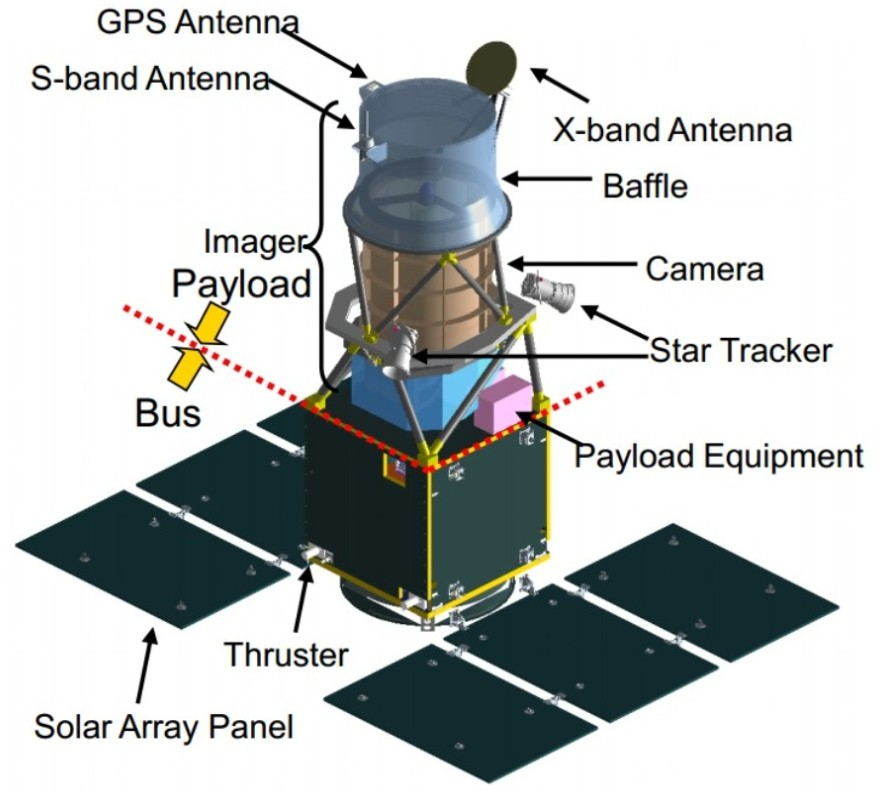
\includegraphics[width=0.8\textwidth]{figures/3.17.jpg}
    			\caption{ASNARO-1 Satellite has many components that have unobstructed views or access to the space environment, like the star tracker, 					camera, imager, and antennas” Image Courtesy of NEC.}
    			\label{fig:communication2}
			\end{figure}
    	\begin{figure}[H]
    		\centering
    		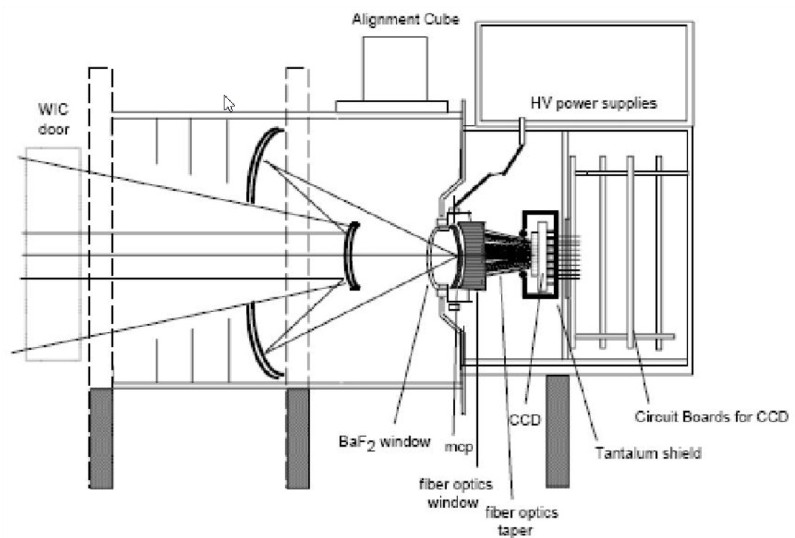
\includegraphics[width=0.8\textwidth]{figures/3.18.jpg}
    		\caption{Schematic view of the Wideband Imaging Camera (WIC) instrument, showing the placement of the power supply with respect to the 							instrument. Image courtesy of UCB/SSL.}
    		\label{fig:communication2}
	\end{figure}
    \item \textbf{Puissance} : la charge utile peut nécessiter :
    \begin{itemize}
        \item Une \textbf{puissance moyenne orbitale} et une \textbf{puissance de crête} adaptées à la distribution électrique (\textit{câblage, carte 					mère et contrôle des cartes filles}).  
        \item Une quantité spécifique de \textbf{puissance générée et/ou stockée} (\textit{taille des panneaux solaires et des batteries}).  
        \item Une \textbf{conversion de tension} et des \textbf{limites de tension} (\textit{conception des circuits imprimés}).  
        \item Une \textbf{régulation du courant} et des \textbf{limites de courant} (\textit{conception des circuits imprimés}).  
    \end{itemize}
    \item \textbf{Commande et Traitement des Données} : la charge utile peut nécessiter :
    \begin{itemize}
        \item Une \textbf{vitesse de traitement} suffisante (\textit{processeurs embarqués : CPU, GPU, RAM}).  
        \item Une \textbf{capacité de stockage des données} adéquate (\textit{mémoire embarquée : carte SD, disque dur}).  
        \item Un \textbf{format de données spécifique} (\textit{image, spectres de fréquence}).  
        \item Une \textbf{bande passante} suffisante pour le transfert des données (\textit{algorithmes pour éviter la surcharge mémoire}).  
        \item Une \textbf{résolution des données} adaptée (\textit{nombre de chiffres significatifs à conserver dans les mesures}).  
    \end{itemize}

    \item \textbf{Communications} : la charge utile peut nécessiter :
    \begin{itemize}
        \item Un \textbf{bilan de liaison} fiable avec une marge suffisante (\textit{transmission bidirectionnelle stable}).  
        \item Un \textbf{débit de liaison montante} adapté (\textit{modes critiques de fonctionnement durant la mission}).  
        \item Un \textbf{débit de télémétrie en liaison descendante} suffisant (\textit{éviter la saturation de la mémoire embarquée}).  
    \end{itemize}
    \item \textbf{Détermination, Contrôle d'Attitude et Navigation} : la charge utile peut nécessiter :
    \begin{itemize}
        \item Une \textbf{précision et exactitude} dans le pointage, le pivotement ou le suivi (\textit{systèmes de contrôle du moment angulaire}).  
        \item Une \textbf{résolution spécifique} dans l'estimation de l'attitude ou de la position (\textit{algorithmes d'estimation, capteurs}).  
    \end{itemize}
\end{itemize}
\textbf{Lectures Suggérées :}  
\textit{\href{https://trs.jpl.nasa.gov/bitstream/handle/2014/41915/11-0422.pdf?sequence=1}
{Instrument Pointing Capabilities: Past, Present, and Future}}

\begin{figure}[H]
    	\centering
    	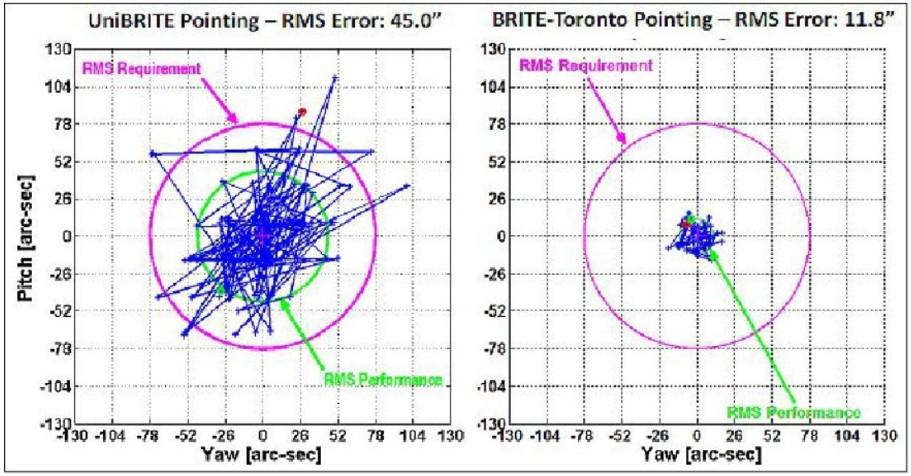
\includegraphics[width=0.8\textwidth]{figures/3.19.jpg}
    	\caption{The primary mission objective of BRITE Constellation is to provide milli-magnitude differential photometry of bright stars. On-orbit fine pointing performance of UniBRITE spacecraft (left) and BRITE-Toronto spacecraft (right)}
    	\label{fig:communication2}
\end{figure}
\textbf{Impact de la Charge Utile sur le Sous-Système Thermique}
\begin{itemize}
    \item \textbf{Thermique} : la charge utile peut nécessiter :
    \begin{itemize}
        \item Une \textbf{plage de fonctionnement thermique spécifique} (\textit{les systèmes optiques, par exemple, préfèrent être maintenus à basse température}).  
        \item Une \textbf{stabilité structurelle face aux variations de température} :
        \begin{itemize}
            \item Utilisation de \textbf{matériaux résistants à la dilatation thermique}.  
            \item Maintien d’une \textbf{température stable} pour éviter les déformations mécaniques.  
        \end{itemize}
    \end{itemize}
\end{itemize}
\begin{figure}[H]
    	\centering
    	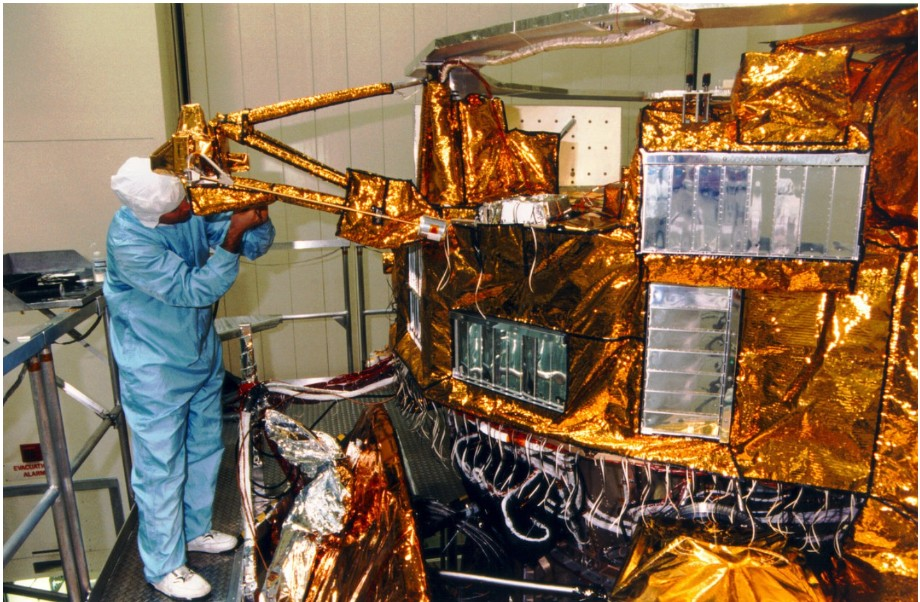
\includegraphics[width=0.8\textwidth]{figures/3.20.jpg}
    	\caption{A unique combination of meticulous old-world skills and high-tech materials produced the finely sewn, super-strong, and extremely lightweight thermal blankets that protected Cassini from the extreme hot and cold of deep space. Image courtesy of NASA.}
    	\label{fig:communication2}
\end{figure}

\section{L'Environnement Spatial et ses Effets sur les Engins Spatiaux}

\subsection{Comparaison entre l’Environnement Terrestre et Spatial}
L’environnement terrestre et spatial présentent à la fois des similitudes et des différences fondamentales. La limite entre ces deux milieux est définie par la ligne de Kármán.

\subsubsection{Similitudes}
\begin{itemize}
    \item Présence de rayonnement électromagnétique
    \item Influence de la gravité
    \item Interaction avec des particules atmosphériques
\end{itemize}

\subsubsection{Spécificités de l’Environnement Spatial}
\begin{itemize}
    \item Radiation cosmique
    \item Plasma et vent solaire
    \item Vide spatial
    \item Micrométéoroïdes et débris orbitaux
\end{itemize}

\subsection{Étude de l’Environnement Spatial}
Plusieurs satellites collectent des données sur la météorologie spatiale :
\begin{itemize}
    \item \textbf{DMSP} : Satellites météorologiques de défense
    \item \textbf{ACE} : Exploration avancée de la composition spatiale
    \item \textbf{SOHO} : Observation du Soleil et de l’héliosphère
    \item \textbf{GOES} : Satellites météorologiques opérationnels géostationnaires
    \item \textbf{TRACE} : Observation de la région de transition et de la couronne solaire
    \item \textbf{SMM} : Mission d’étude des maxima solaires
\end{itemize}

\subsection{L’Influence du Soleil sur l’Environnement Spatial}
Le Soleil impacte les engins spatiaux à travers plusieurs phénomènes :
\begin{itemize}
    \item Vent solaire
    \item Flux d’ondes radio
    \item Éruptions solaires et éjections de masse coronale (CME)
    \item Chauffage coronarien
    \item Taches solaires
    \item Rayonnement électromagnétique (UV, rayons X, gamma)
\end{itemize}

\subsubsection{Effets du Rayonnement Solaire sur les Engins Spatiaux}
\begin{itemize}
    \item Dégradation des panneaux solaires et des matériaux polymères
    \item Perturbations d’attitude
    \item Décroissance orbitale en raison du chauffage atmosphérique
    \item Interférences avec les transmissions radio
\end{itemize}

\subsubsection{Rayonnement Électromagnétique}
Le Soleil émet un large spectre d’ondes électromagnétiques, influençant les satellites et autres engins spatiaux.
\begin{itemize}
    \item \textbf{Rayonnement ultraviolet (UV)} : Chauffage atmosphérique, fragilisation des matériaux
    \item \textbf{Rayons X} : Perturbation des communications et des systèmes électroniques
    \item \textbf{Rayons gamma} : Indicateurs précoces d’éruptions solaires majeures
\end{itemize}

\subsection{Le Chargement Électrostatique des Satellites}
\subsubsection{Chargement de Surface}
\begin{itemize}
    \item \textbf{En éclipse} : Accumulation de charge électrostatique (jusqu’à plusieurs kilovolts)
    \item \textbf{En plein Soleil} : Photoémission d’électrons créant une charge positive
    \item \textbf{Facteurs déclencheurs des décharges} :
    \begin{itemize}
        \item Variation de l’illumination solaire
        \item Modification de l’environnement particulaire
        \item Activité électrique embarquée
    \end{itemize}
\end{itemize}

\subsection{Impacts à Haute Vitesse sur les Satellites}
Les satellites en orbite terrestre sont exposés à des impacts de haute vitesse de :
\begin{itemize}
    \item Débris spatiaux (d’origine humaine)
    \item Météoroïdes et micrométéoroïdes (naturels)
\end{itemize}

\subsubsection{Débris Spatiaux}
\begin{itemize}
    \item Sources : satellites hors service, collisions, explosions
    \item Nombre suivi : ~23 000 objets catalogués (CSpOC - USA)
    \item Vitesse moyenne d’impact : ~10 km/s
    \item Menace principale : impacts de petits débris (mm-cm)
\end{itemize}

\subsubsection{Dommages Causés}
\begin{itemize}
    \item Spallation : Détachement de particules à l’impact
    \item Cratérisation : Déformation de la surface
    \item Pénétration : Perforation des parois
    \item Fragmentation : Rupture sous un impact énergétique élevé
\end{itemize}

\subsubsection{Détection et Suivi des Débris}
\begin{itemize}
    \item Radars et télescopes terrestres (ex. radar Haystack - USAF/NASA)
    \item Inspection des satellites retournés sur Terre
\end{itemize}

\subsubsection{Protection des Satellites contre les Impacts}
\begin{itemize}
    \item Blindage Whipple : Bouclier multicouche absorbant l’énergie des impacts
    \item Orientation stratégique : Minimisation de l’exposition
    \item Respect des réglementations (NASA, NOAA, DOD, traités internationaux)
\end{itemize}

\subsection{Conclusion}
L’environnement spatial présente de nombreux défis pour les satellites, notamment le rayonnement solaire, le chargement électrostatique et les impacts de haute vitesse. Une surveillance rigoureuse et une conception optimisée sont essentielles pour assurer la longévité et la fonctionnalité des missions spatiales.




%\chapter{Communication} 
%\section{Définition} % 1.1
Le sous-système de communication d'un vaisseau spatial combine la liaison de communication entre le vaisseau spatial et le sol. Des antennes et des émetteurs-récepteurs sont présents à la fois sur le vaisseau spatial et au sol pour transmettre et recevoir des signaux. L'objectif ultime est de garantir une liaison de communication entre le vaisseau spatial et le centre de contrôle de mission pour les phases requises de la mission afin de télécharger des données de charge utile propres et de charger les commandes du vaisseau spatial.

\begin{figure}[H] % H force l'affichage ici
    \centering
    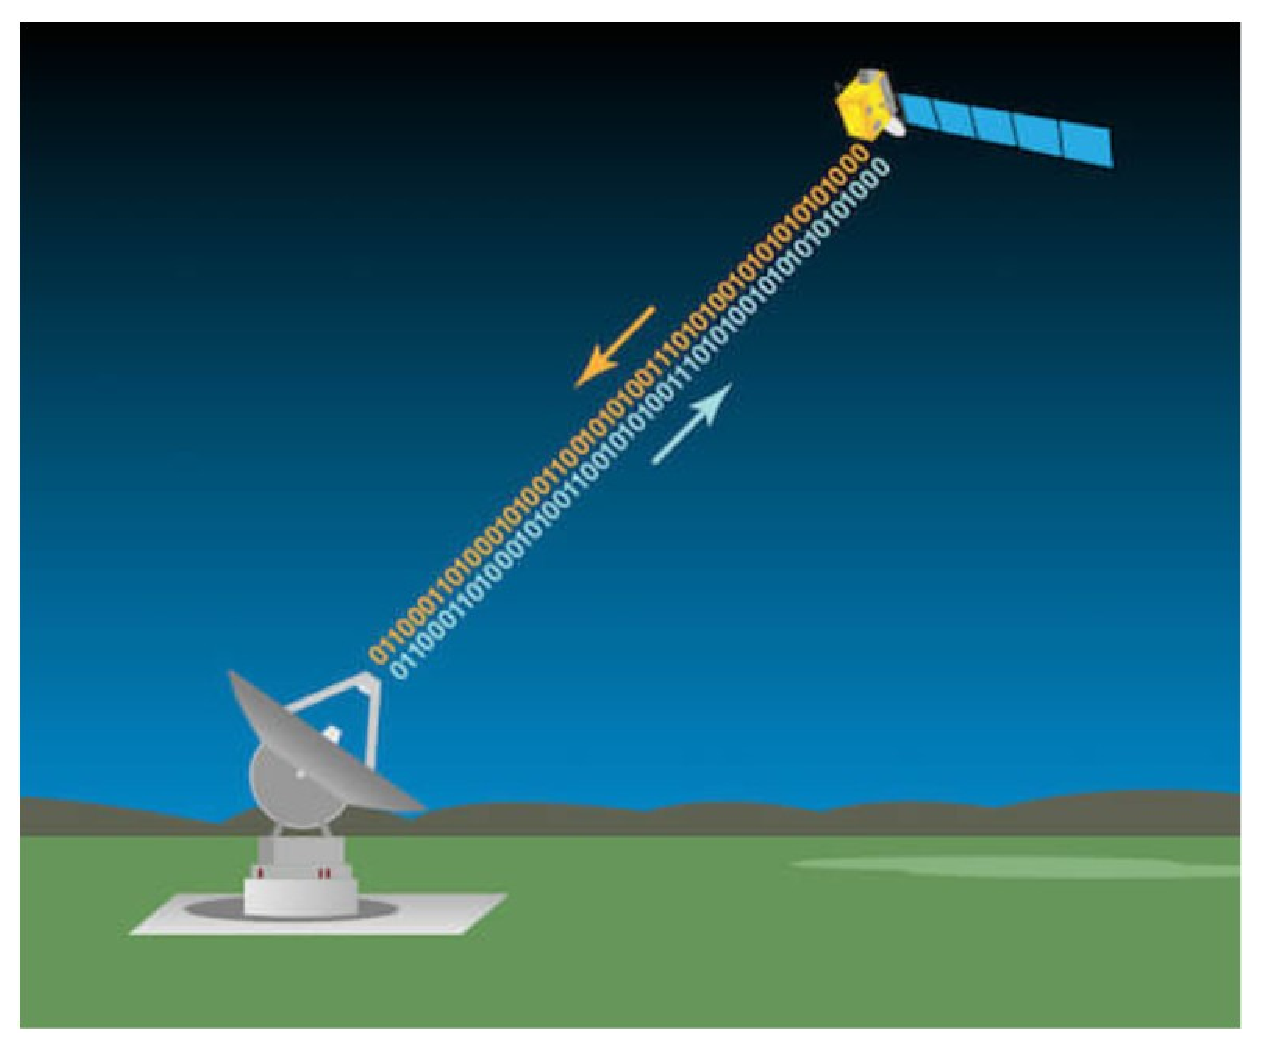
\includegraphics[width=0.5\textwidth]{figures/6-1.eps}
    
    \caption{Illustration d'un vaisseau spatial envoyant et recevant des informations d'une antenne DSN. Crédit image : NASA/JPL-Caltech..}
    \label{fig:communication}
\end{figure}
  % In
%\section{Responsabilités du sous-système} % 1.1
Le sous-système de communication est responsable des fonctions suivantes :

\renewcommand{\labelitemi}{$\bullet$}
\begin{itemize}
    \item \textbf{Transmission des données de charge utile} vers le sol, en fonction des exigences de la mission.
    \item \textbf{Adaptabilité à la mission}, offrant une large gamme de débits de données, de bandes passantes et de niveaux de criticité.
    \item \textbf{Envoi des données du vaisseau spatial} vers le sol pour les opérations, notamment :
    \begin{itemize}
    		
        \item \textbf{Données d’attitude et d’accélération} : issues de capteurs solaires, capteurs stellaires, gyroscopes, accéléromètres, etc.
        \item \textbf{Données de maintenance} : incluant les températures, pressions, tensions, courants, etc.
    \end{itemize}
    
    \item \textbf{Réception des commandes} transmises depuis le sol pour le pilotage et l'exploitation du vaisseau spatial.
\end{itemize}

\begin{figure}[H] % H force l'affichage ici
    \centering
    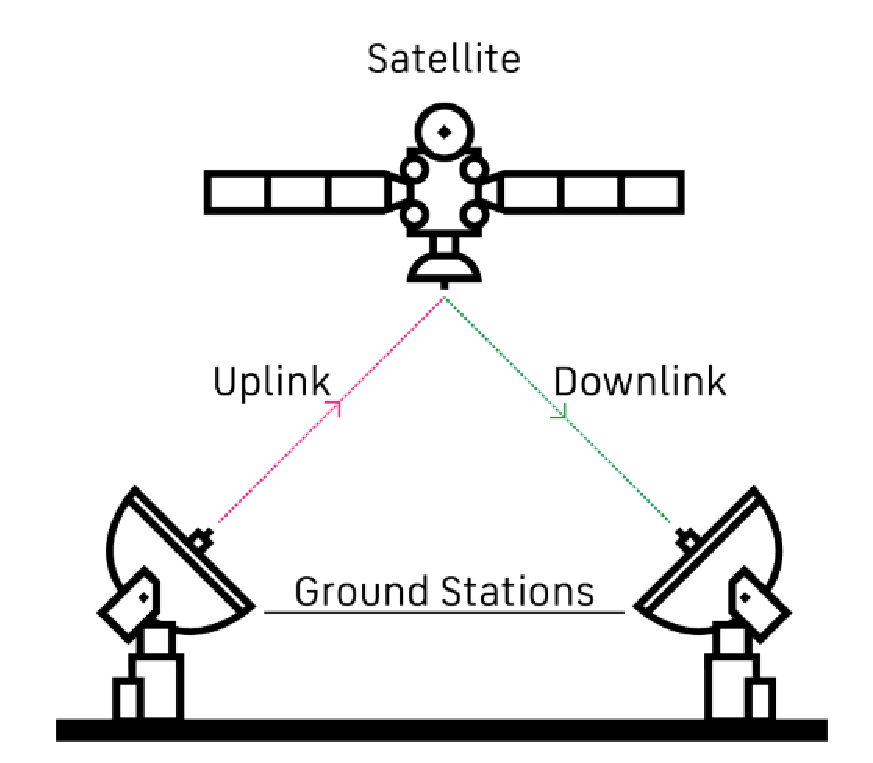
\includegraphics[width=0.5\textwidth]{figures/6-120.eps}
    
    \caption{Un scénario de communication par satellite de base. Le satellite relaie les signaux reçus vers les segments terrestres situés dans son empreinte. Image d'Inmarsat}
    \label{fig:communication2}
\end{figure}



\begin{itemize}
    \item Définition d'une architecture de communication, qui comprend le bus spatial et les segments terrestres.
    \begin{itemize}
        \item Sélection d'une fréquence radio et obtention de la licence pour cette radiofréquence.
        \item Jongler avec le nombre et la position des stations terrestres disponibles
    \end{itemize}
    \item Sélection et codage de la compression, de l'encodage et de la modulation des signaux pour équilibrer la perte et la bande passante.
    \item Sélectionnez une technologie de communication qui respecte les contraintes de masse, de volume, de puissance et les réglementations et qui répond aux exigences de la mission
    \item Vérification de la fermeture du budget de liaison de communication en fonction des technologies sélectionnées et de l'architecture de la station au sol   
\end{itemize}





 
%\section{Processus de conception général} 
Compte tenu de la charge utile et des données de maintenance nécessaires pour la liaison descendante depuis le satellite, le spécialiste COMMS doit définir une architecture de communication avec de nombreux paramètres libres. Le processus est le suivant :

\begin{enumerate}
\item Choisissez une fréquence radio. Cette fréquence détermine la bande passante maximale disponible et dépend de la classe de la mission. De nombreuses missions CubeSat utilisent des fréquences de classe amateur ou expérimentale .

\begin{figure}[H] % H force l'affichage ici
    \centering
    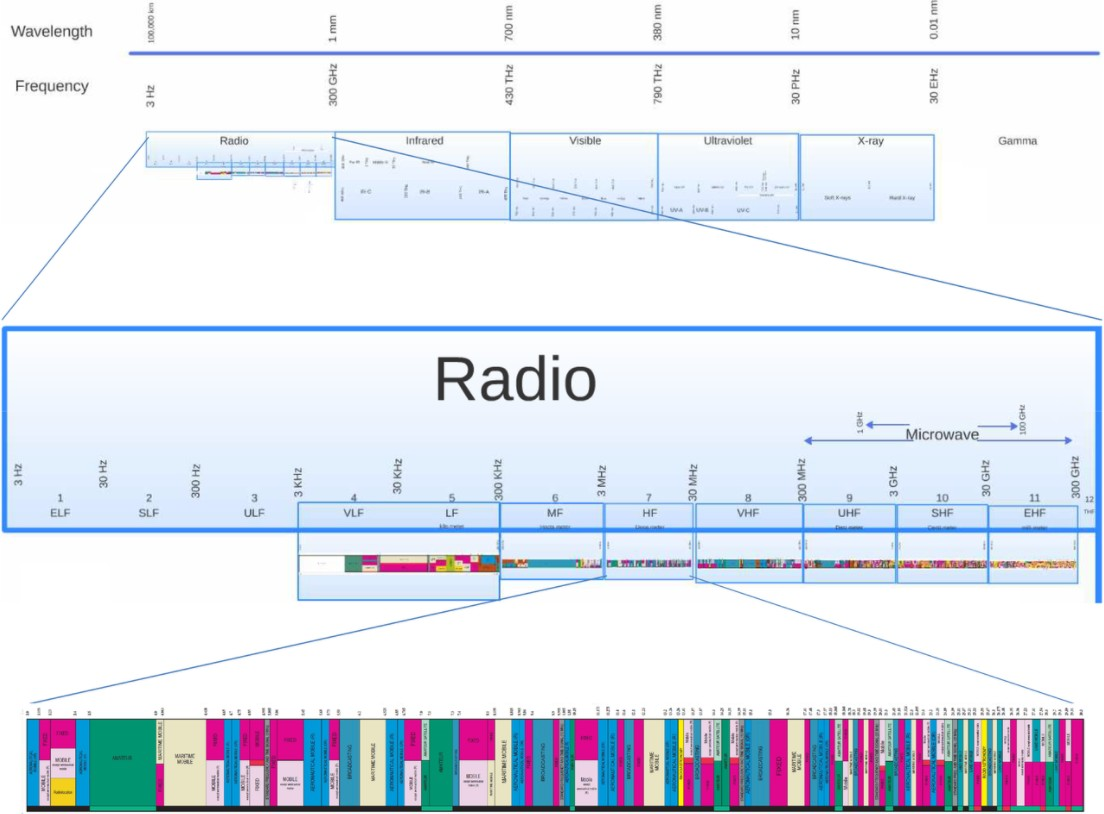
\includegraphics[width=0.5\textwidth]{figures/6-5.jpg}
    
    \caption{Haute fréquence : une vue d'ensemble de la position des hautes fréquences dans l'ensemble du spectre électromagnétique. Image d'Arkrishna.}
    \label{fig:communication2}
\end{figure}

\item Choisissez un schéma de modulation. Le schéma de modulation détermine le rapport signal/bruit requis.

\item Choisissez des algorithmes de codage qui affectent non seulement le rapport signal/bruit mais également le débit de données.
\item Analysez le temps de contact disponible que le satellite obtiendra en utilisant les stations terrestres disponibles, l'orbite et la conception de la constellation, le cas échéant. Le temps de contact est directement proportionnel à la rapidité avec laquelle le vaisseau spatial peut transmettre des données et à la fréquence à laquelle les opérateurs de mission peuvent émettre des commandes.


\end{enumerate}

Après avoir défini plusieurs options pour chaque aspect de l’architecture de communication, pour chaque alternative :

\begin{enumerate}
\item Calculer le débit de données requis à partir de toutes les sources (en fonction de l'orbite)
\item Utilisez l'équation du bilan de liaison pour dimensionner l'antenne/l'émetteur afin d'avoir une marge suffisante sur le rapport signal/bruit. Cela garantit que toutes les alternatives répondent aux exigences

\end{enumerate}
Une fois les architectures alternatives définies, utilisez d'autres mesures telles que le coût total du sous-système ou le risque pour sélectionner une alternative. Remarque : il s'agit souvent d'un processus itératif et nous pouvons modifier nos exigences en fonction de la faisabilité.

%\section{Exigences typiques et considérations de conception}
Pour la mission spatiale, le système de communication doit être conçu pour répondre aux besoins de liaison montante et descendante des données de la charge utile et du bus du vaisseau spatial. Les exigences comprennent des spécifications techniques pour :
\begin{itemize}
\item Avant tout, le système de communication dans son ensemble doit avoir un bilan de liaison qui se ferme et, de manière optimale, présente une marge positive.
\begin{itemize}
\item Les principaux facteurs qui influencent le bilan de liaison sont la puissance disponible pour la transmission, le gain de l'antenne (géométrie et masse), la température des composants et l'orbite (pertes). Ces paramètres seront développés dans la section sur les bilans de liaison.
\item Les pertes du système proviennent de la température des composants. Le sous-système thermique peut devoir respecter les exigences imposées par le sous-système de communication.
\end{itemize}
\begin{figure}[H] % H force l'affichage ici
    \centering
    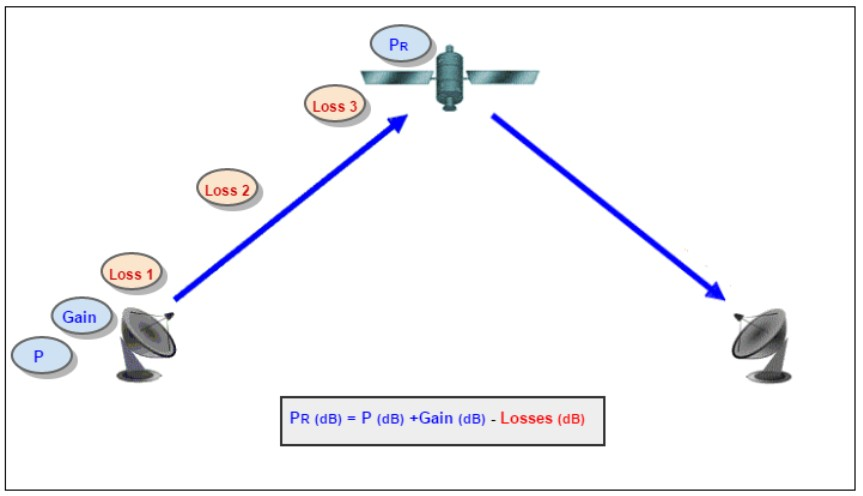
\includegraphics[width=0.8\textwidth]{figures/6-6.jpg}
        \caption{Gain de l'amplificateur de l'émetteur et du récepteur. Atténuation dans la propagation dans l'atmosphère. Pertes de dépointage. Pertes dues à la désadaptation de polarisation. Pertes dans les équipements de transmission et de réception. Image de Source Forge.}
    \label{fig:communication2}
\end{figure}
\item Débit de données entre le vaisseau spatial et la station au sol pour la transmission des données de charge utile et la transmission des commandes ou des logiciels d'opération de mission. Cette mesure ressemble beaucoup à l'exigence de débit du CDH, mais au lieu de l'interface entre la charge utile et l'ordinateur de vol, le débit de données est l'interface entre le vaisseau spatial et la station au sol.
\item Le temps de contact avec les stations terrestres (et le débit de données) détermine le nombre total de données qu'un vaisseau spatial est capable de transmettre. Le temps de contact dépend du nombre et de l'emplacement des stations terrestres, ainsi que de l'orbite du vaisseau spatial.
\begin{itemize}
\item Étant donné que le vaisseau spatial peut communiquer avec le sol, la charge utile génère une certaine quantité de données qui sont nécessaires à la transmission en liaison descendante pour remplir la mission. Cette exigence de niveau supérieur contribue aux exigences de débit de données et de temps de contact.

\end{itemize}
\begin{figure}[H] % H force l'affichage ici
    \centering
    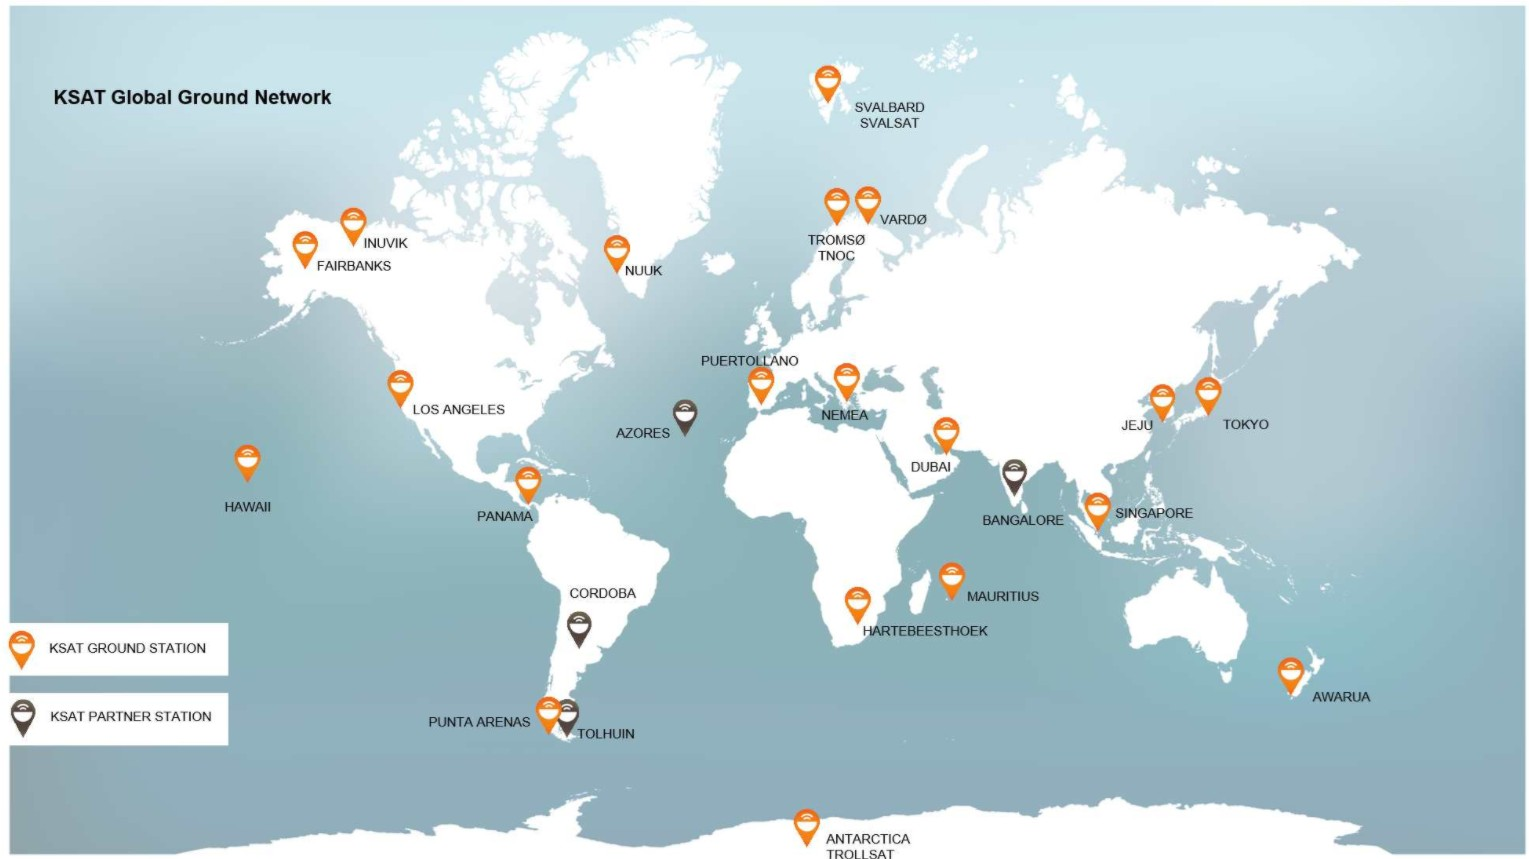
\includegraphics[width=0.8\textwidth]{figures/6-7.jpg}
    
    \caption{KSAT vous donne accès à notre vaste réseau terrestre mondial composé de stations situées aux deux pôles et à des emplacements triés sur le volet à moyenne latitude pour garantir un accès continu à vos satellites. Image de KSAT.}
    \label{fig:communication2}
\end{figure}
\item La directionnalité (omnidirectionnelle ou directionnelle) de l'antenne détermine l'obligation du système de détermination et de contrôle d'attitude de pointer le vaisseau spatial pendant les communications. Cette manœuvre de pointage affecte également la manière dont nous effectuons les opérations de mission.
\begin{figure}[H] % H force l'affichage ici
    \centering
    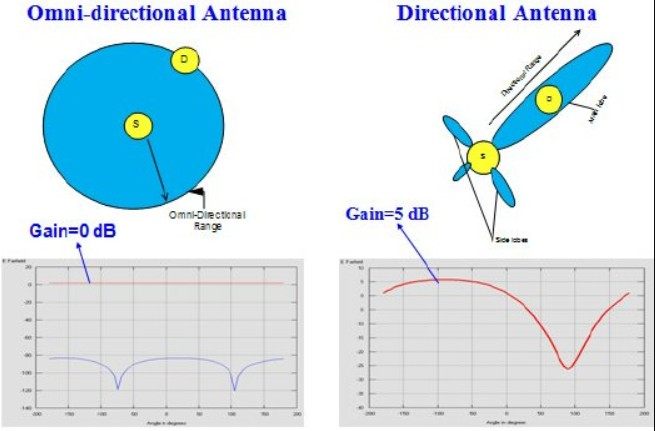
\includegraphics[width=0.8\textwidth]{figures/6-8.jpg}
    \caption{Diagrammes de rayonnement des antennes omnidirectionnelles et directionnelles.}
    \label{fig:communication2}
\end{figure}
\item Le chercheur principal peut imposer une quantité suffisante de bruit ou de perte de signal. Le spécialiste des communications doit alors tenir compte de ce bruit ou de cette perte dans la conception du codage et de la modulation.
\end{itemize}
\textbf{Documents requis}
\begin{itemize}
    \item La spécification de conception CubeSat Rev. 14 impose des exigences en matière de licences radio :
    \begin{itemize}
        \item \textbf{Obtention des licences} :
        \begin{itemize}
            \item Les opérateurs doivent obtenir et fournir la documentation relative aux licences appropriées pour l’utilisation des fréquences radio.
            \item \textit{Remarque} : Pour l'utilisation de fréquences amateurs, il faut prouver que la fréquence a été coordonnée par l'IARU. Les demandes peuvent être consultées sur \url{https://www.iaru.org}.
        \end{itemize}
        \item \textbf{Conformité aux réglementations nationales} :
        \begin{itemize}
            \item Les CubeSats doivent respecter les accords et restrictions de licence radio de leur pays.
            \item \textit{Remarque} : Les opérateurs CubeSat doivent se référer à l'Union internationale des télécommunications (UIT) pour déterminer les licences et les approbations nécessaires pour leur pays.
        \end{itemize}
    \end{itemize}
\end{itemize}
\begin{itemize}
    \item Le temps entre le déploiement et la transmission par radiofréquence est exigé en externe par les fournisseurs de lancement.
    \begin{itemize}
        \item L'IDD du déployeur CubeSat externe NanoRacks spécifie dans les commutateurs de déploiement:
        \item 4.1.4-5) Les commutateurs de déploiement du CubeSat doivent réinitialiser la charge utile à l'état de pré-lancement s'ils sont actionnés à tout moment dans les 30 premières minutes après la fermeture des commutateurs (y compris, mais sans s'y limiter, la transmission radiofréquence et les minuteries du système déployable).
     \end{itemize}
    \item Le nombre de stations terrestres auxquelles vous avez accès et le niveau d'accès dont vous disposez. À moins que vous n'ayez construit votre propre station terrestre, vous devrez probablement utiliser la station terrestre ou le réseau de quelqu'un d'autre. Travailler avec d'autres personnes comporte des contraintes qui dépendent de leur disponibilité, de leur coût et de votre relation avec l'organisme de contrôle.
    \begin{itemize}
        \item Réseau de stations terrestres internationales (IGS) exploité par notre réseau de stations terrestres américaines et internationales (IC).
        \item Station terrestre Amazon Web Services sous Amazon.
        \item SatNOGS, un réseau mondial open source de stations terrestres par satellite, détenu et exploité par la communauté.
    \end{itemize}
\end{itemize}
\begin{figure}[H] % H force l'affichage ici
    \centering
    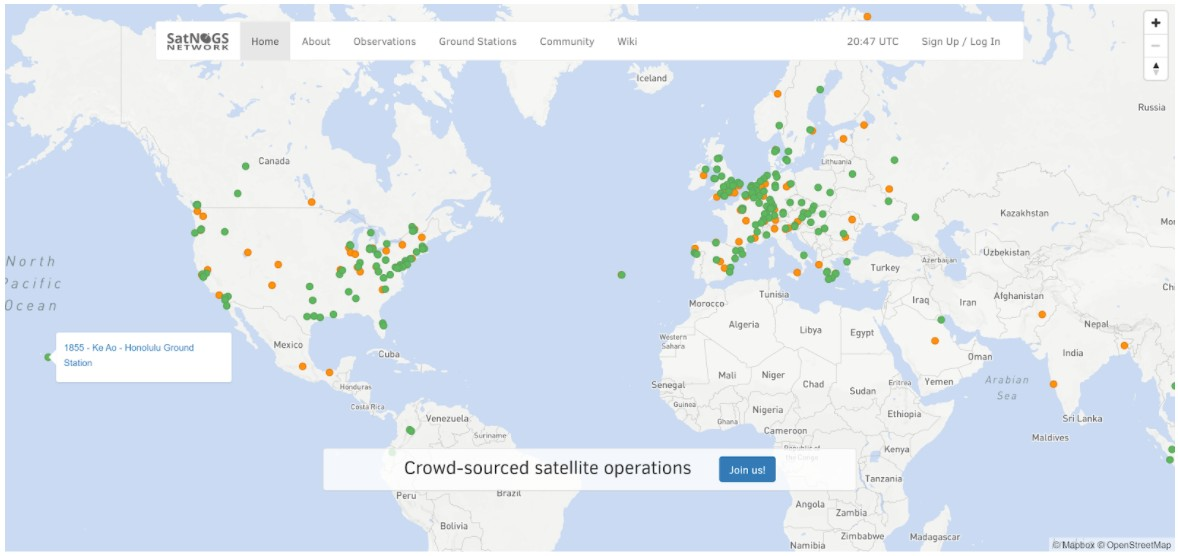
\includegraphics[width=0.8\textwidth]{figures/6-10.jpg}
    
    \caption{Réseau SatNOGS actuel au 17/12/2020 à 10h47 HST. Image de Satnogs Network.}
    \label{fig:communication2}
\end{figure}
Lors de la fabrication et de l'assemblage, vous, en tant que spécialiste des communications, devez manipuler plusieurs composants, allant de la carte de communication à l'antenne, en passant par les amplificateurs, les radios, etc. Vous travaillerez probablement avec le spécialiste des systèmes d'alimentation, car le système de communication est gourmand en énergie. La manipulation des systèmes de communication suit les meilleures pratiques des composants des systèmes d'alimentation électrique.
\begin{figure}[H] % H force l'affichage ici
    \centering
    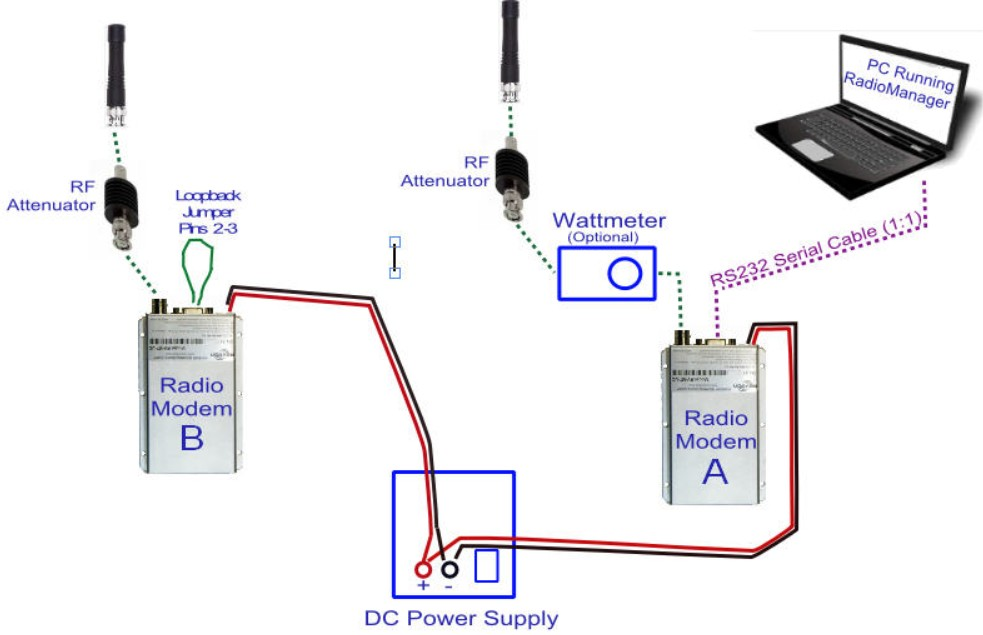
\includegraphics[width=0.8\textwidth]{figures/6-11.jpg}
    
    \caption{Test radio en plein air ou test de liaison, qui effectue les opérations suivantes : Capture de la configuration/des paramètres du modem radio dans un fichier. Vérification que le modem radio transmet le niveau de puissance de sortie RF correct. La fréquence du modem radio est correctement définie. Les paramètres du port série sont corrects. Le débit en bauds en direct est correct et compatible avec le système dans lequel le modem sera utilisé. Vérification et enregistrement de la consommation d'énergie CC. Détermination du taux d'erreur de paquets sur le banc ou sur le terrain. Image de Raveon.}
    \label{fig:communication2}
\end{figure}

Lors des tests, le logiciel de codage et de modulation doit être chargé et testé avec le matériel. Pour vérifier les communications de bout en bout entre la radio du vaisseau spatial et votre récepteur, une distance appropriée est placée entre la radio et le récepteur, et les pertes qui se produiraient entre l'espace et le sol sont simulées par des atténuateurs, fixés à chaque extrémité [ NASA MAVEN ]. Les signaux sont surveillés sur un ordinateur pour voir 1) si les signaux sont captés et 2) la quantité de perte dans les signaux reçus. L'intégration de ce code dans le logiciel général du vaisseau spatial impliquera le spécialiste du commandement et du traitement des données.

Pendant le transport et la manutention, l'ordinateur de vol est éteint et autonome dans le satellite. Le spécialiste des communications n'a aucune exigence à respecter à ce stade.
\begin{figure}[H] % H force l'affichage ici
    \centering
    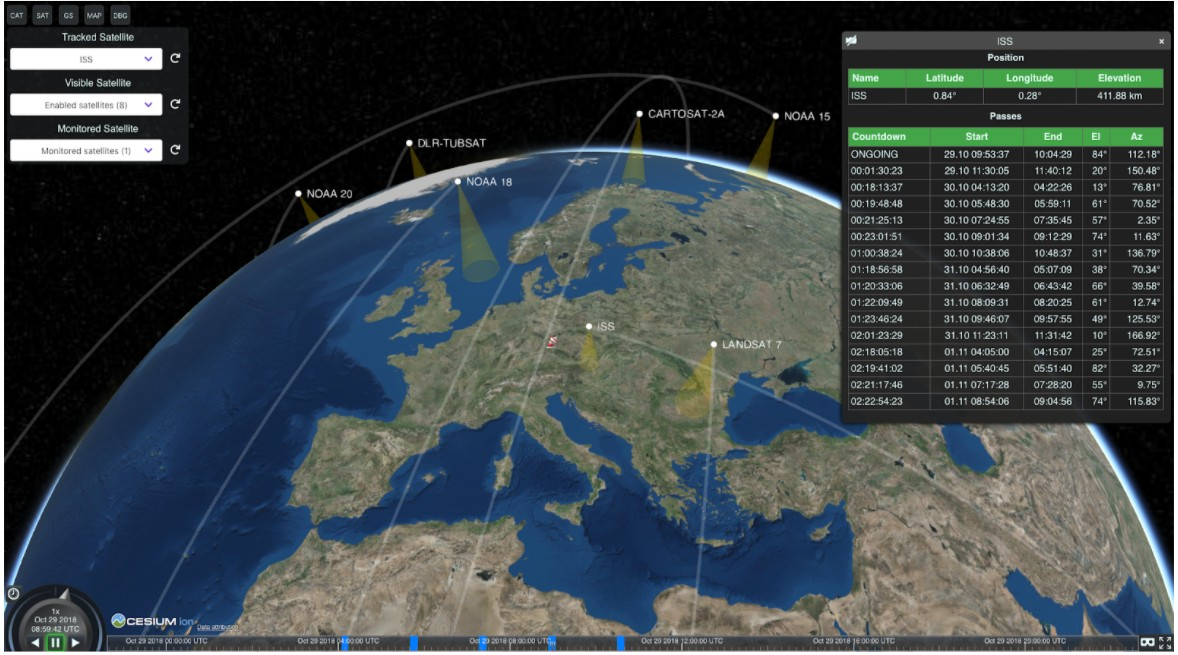
\includegraphics[width=0.8\textwidth]{figures/6-12.jpg}
    
    \caption{Visualisation de l'orbite des satellites et prédiction de leur passage. Image de Florian Mauracher sur Github.}
    \label{fig:communication2}
\end{figure}
Depuis la livraison jusqu'au déploiement en orbite, le spécialiste des communications doit s'assurer que le logiciel de suivi d'orbite et de station au sol est prêt à fonctionner. Une fois le vaisseau spatial déployé, le spécialiste des communications doit mettre à jour les éléments orbitaux (TLE ) dans son logiciel de station au sol afin que la station au sol directionnelle puisse s'orienter avec précision dans la direction du vaisseau spatial. Pour les stations au sol omnidirectionnelles ou directionnelles, la mise à jour des TLE informera les opérateurs de mission du moment où le vaisseau spatial passe au-dessus de leur tête dans une zone de portée communicable.
\begin{center}
    \textbf{Kit Artemis spécifique}
\end{center}
\begin{itemize}
    \item \textbf{Système de communication CubeSat} :
    \begin{itemize}
        \item Le système de communication CubeSat transmettra la télémétrie depuis l'orbite terrestre basse (LEO).
        \item \textbf{Exigences de transmission} :
        \begin{itemize}
            \item La radio doit transmettre une télémétrie détectable en fréquence radio amateur (UHF).
            \item Les stations au sol recevront le signal UHF et traiteront la télémétrie réelle.
            \item Le bilan de liaison doit avoir une marge d'au moins 5 dB.
        \end{itemize}
    \end{itemize}
\end{itemize}
\begin{center}
    \textbf{Activité suggérée}
\end{center}
« Quelles exigences de communication devez-vous imposer à votre système pour remplir votre mission scientifique ? »
 




%\section{Exigences typiques et considérations de conception}
Le sous-système de communications est un élément clé d'un satellite, car il est directement lié aux autres sous-systèmes, notamment :

- La charge utile (Payload) → Le sous-système de communication permet la transmission des données générées par la charge utile (ex : images, mesures scientifiques).

- Le sous-système de commande et de gestion des données (CDH - Command and Data Handling) → Il gère l’échange d’informations entre les différents sous-systèmes et assure la bonne exécution des commandes envoyées depuis la Terre.

- L’orbite du satellite → L’orbite détermine le temps de contact avec les stations terrestres, ce qui influence la capacité de transmission et réception des données.

- Le segment sol (stations terrestres) → Il permet de communiquer avec le satellite pour recevoir les données et envoyer des commandes.
\begin{figure}[H] % H force l'affichage ici
    \centering
    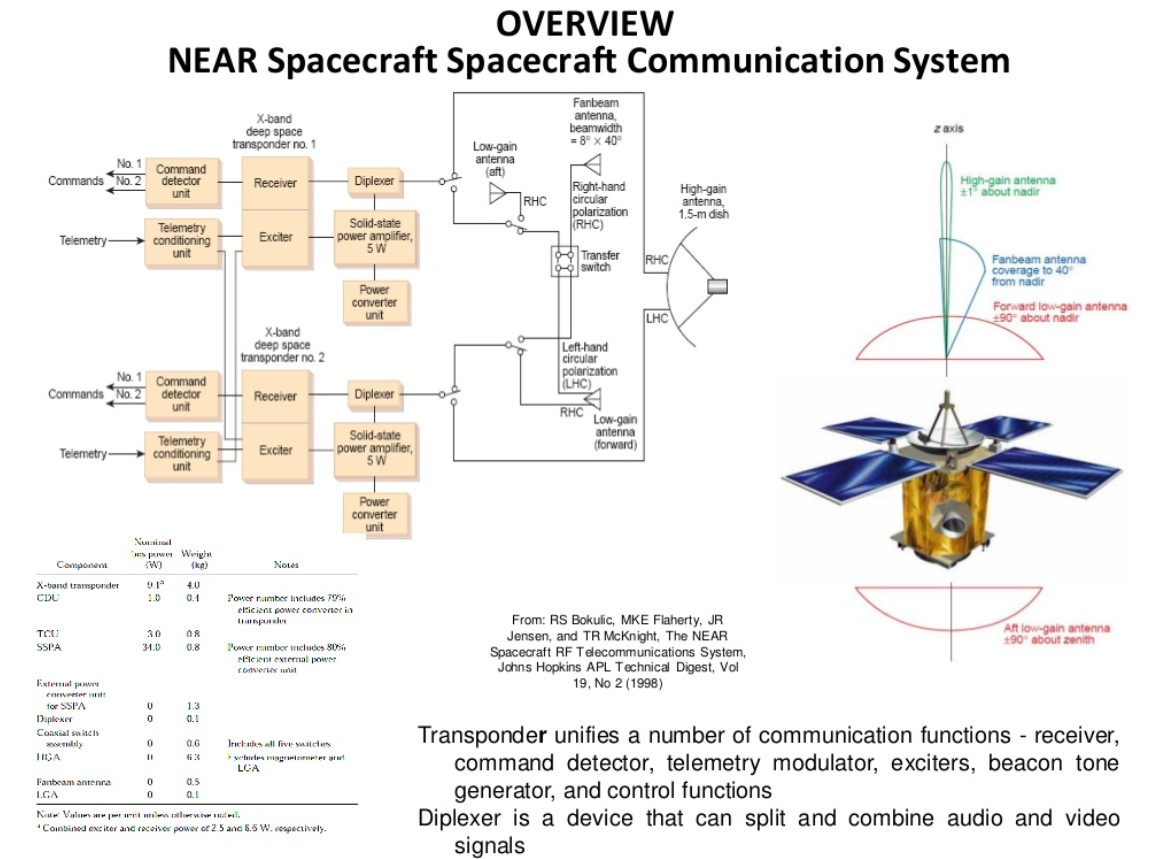
\includegraphics[width=0.8\textwidth]{figures/6-13.jpg}
    
    \caption{Présentation du système de communication du vaisseau spatial NEAR. Image de Pisacane.}
    \label{fig:communication2}
\end{figure}
Les \textbf{antennes} doivent être \textbf{dégagées de tout obstacle} pour assurer une bonne émission et réception des signaux. Elles peuvent être :
\begin{itemize}
    \item \textbf{Omnidirectionnelles} : émettant dans toutes les directions.
    \item \textbf{Directionnelles} : orientées vers une cible spécifique.
\end{itemize}
Les composants internes du sous-système de communication sont regroupés sur une \textbf{carte de communication} contenant :
\begin{itemize}
    \item \textbf{Amplificateurs} : Augmentent la puissance du signal.
    \item \textbf{Filtres} : Suppriment les interférences.
    \item \textbf{Diplexeurs} : Permettent d'utiliser une même antenne pour émettre et recevoir.
    \item \textbf{Récepteurs} : Captent les signaux venant du sol.
\end{itemize}
Cette carte est reliée à l’\textbf{ordinateur central} du satellite, contrôlé par le \textbf{sous-système de gestion des commandes et des données (CDH)}.Cette liaison permet:
\begin{itemize}
    \item \textbf{D'envoyer les commandes} depuis la Terre.
    \item \textbf{De transmettre les données} de la charge utile vers le sol.
\end{itemize}
Le traitement du signal peut se faire:
\begin{enumerate}[noitemsep, nolistsep]
    \item Directement sur la carte de communication, avec un traitement matériel dédié.
    \item Sur l’ordinateur central, offrant plus de flexibilité avec un traitement logiciel.
\end{enumerate}
Le sous-système de communication combine matériel et logiciel, reliant des antennes externes à une carte électronique dédiée, qui assure l'interface avec l’ordinateur central et le CDH.
\href{https://www.youtube.com/watch?v=NGgzq8eXZOQ&feature=youtu.be}{Deep Space Network: A Discussion on NASA’s Vital Lifeline to Spacecraft. Video by NASA/JPL}
\begin{itemize}[noitemsep, nolistsep]
    \item Responsabilités du spécialiste des communications du bus spatial :
    \begin{itemize}
        \item Il n'est pas responsable du segment sol.
        \item Il doit cependant coordonner avec le responsable du segment sol.
    \end{itemize}
     \item Contexte des réseaux de stations au sol :
    \begin{itemize}
        \item Les grandes agences (ex. NASA) disposent de réseaux comme le Deep Space Network :
        \begin{itemize}
            \item Couvre une large gamme de fréquences.
            \item Offre une couverture continue.
        \end{itemize}
        \item Les petits groupes (universités, entreprises) doivent :
        \begin{itemize}
            \item Construire leur propre réseau de stations au sol.
            \item Acheter un accès à un réseau existant.
        \end{itemize}
    \end{itemize}
    \item \textbf{Réseau SatNOGS :}
    \begin{itemize}
        \item Une \textbf{communauté ouverte} de stations au sol opérées par des passionnés.
        \item Implique des \textbf{opérateurs radioamateurs} du monde entier.
        \item Permet aux \textbf{petits satellites} d’envoyer des données, même sans accès au \textbf{Deep Space Network}.
    \end{itemize}
    \item \textbf{Accessibilité croissante des stations au sol :}
    \begin{itemize}
        \item Comme les engins spatiaux, leur construction et exploitation deviennent \textbf{de plus en plus accessibles}.
        \item Le mouvement \textbf{DIY} facilite leur développement pour les amateurs et passionnés.
    \end{itemize}
\end{itemize}
\begin{figure}[H] % H force l'affichage ici
    \centering
    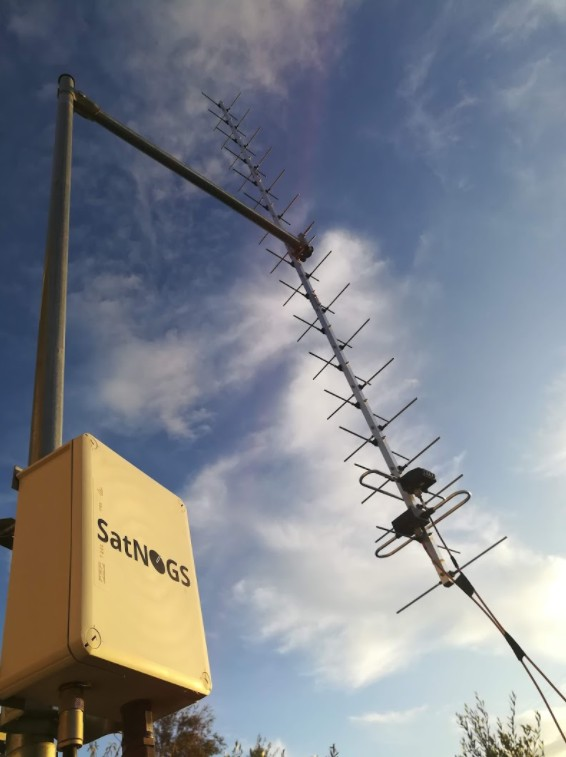
\includegraphics[width=0.8\textwidth]{figures/6-14.jpg}
        \caption{SatNOGS Network – Ground Station Avia. Image by Satnogs Network.}
    \label{fig:communication2}
\end{figure}

%\section{Principes fondamentaux des signaux}
Cette section abordera les principes fondamentaux des signaux, du traitement du signal et des bilans de liaison dans le contexte des engins spatiaux. Nous commencerons par la manière dont les informations sont structurées (niveau bas) jusqu'à la manière dont les informations sont transmises (niveau élevé). Ces concepts sont importants pour votre chercheur principal, qui compte sur vous pour communiquer des données de charge utile de qualité.
\subsection{Signaux analogiques/numériques}
La plupart des informations mesurées et transmises par les satellites sont de nature continue. Par exemple, la luminance spectrale d'une image (données de charge utile) ou la température de la batterie (télémétrie). Les informations peuvent être transmises par des signaux analogiques (continus) ou numériques (discrétisés, bits). La conversion analogique/numérique transforme les quantités continues en bits. Les communications analogiques et numériques sont toutes deux utilisées dans les satellites, mais la plupart des systèmes de communication par satellite actuels sont numériques car les modulations numériques sont généralement plus résistantes au bruit.
\begin{figure}[H] % H force l'affichage ici
    \centering
    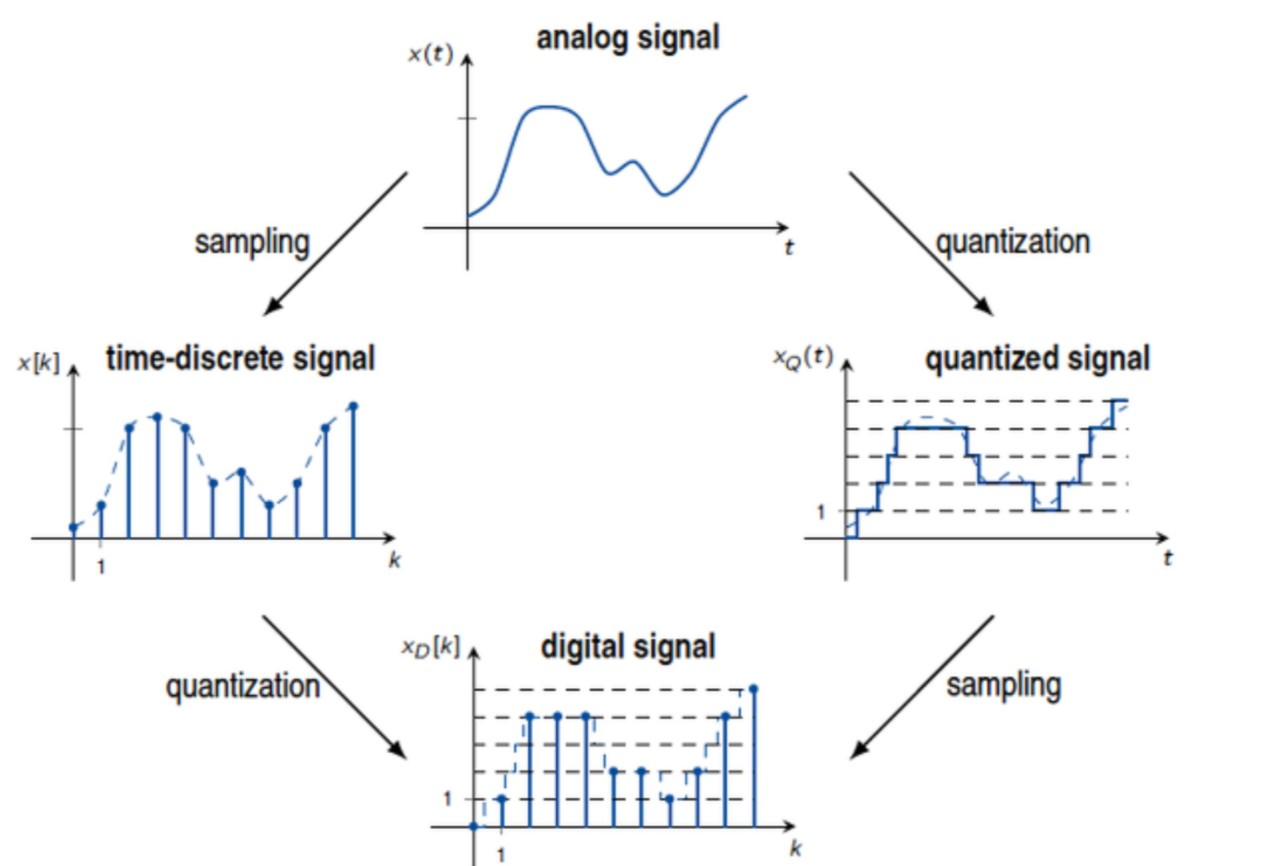
\includegraphics[width=0.8\textwidth]{figures/6-15.jpg}
    \caption{Deux méthodes de conversion de signaux analogiques en signaux numériques. Image de Dan Boschen.}
    \label{fig:communication2}
\end{figure}
\textbf{Quantification}
La quantification est la conversion d'une quantité physique continue (par exemple la tension) en un nombre numérique (bits). Cela implique une quantification, qui introduit une erreur de quantification (d'arrondi). La valeur quantifiée est donnée par l'équation suivante :
\begin{equation}
            Q=\frac{E_{r}}{2^{M}}=\frac{V_{max}-V_{max}}{2^{M}}
\end{equation}
Où $ E_{r} $ est la plage de la variable physique, M est le nombre de bits et V est la variable physique.
\begin{figure}[H] % H force l'affichage ici
    \centering
    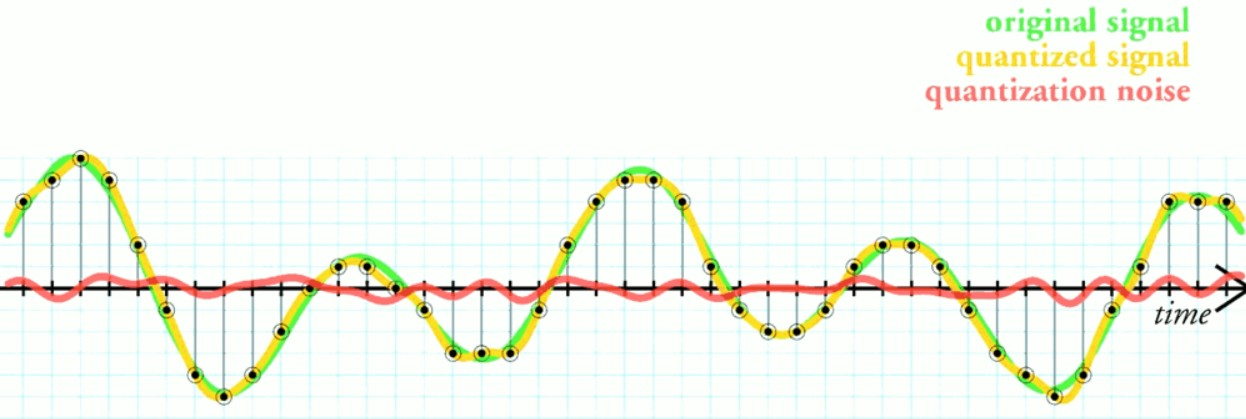
\includegraphics[width=0.8\textwidth]{figures/6-16.jpg}
    \caption{Quantification}
    \label{fig:communication2}
\end{figure}
La manière la plus simple de quantifier un signal consiste à choisir la valeur d'amplitude numérique la plus proche de l'amplitude analogique d'origine. Cet exemple montre le signal analogique d'origine (vert), le signal quantifié (points noirs), le signal reconstruit à partir du signal quantifié (jaune) et la différence entre le signal d'origine et le signal reconstruit (rouge). La différence entre le signal d'origine et le signal reconstruit est l'erreur de quantification et, dans ce schéma de quantification simple, est une fonction déterministe du signal d'entrée. Image de Gregory Maxwell.
Un exemple illustratif : disons que nous avons des mesures de température allant de \(-100^\circ C\) à \(+100^\circ C\).  
Si nous les codons avec seulement 3 bits, cela définit 8 niveaux.  
Le pas de quantification est donné par :
\[
\Delta T = \frac{200^\circ C}{8} = 25^\circ C
\]
\noindent Ce qui signifie :
\begin{itemize}
    \item Toute température comprise entre \(-100^\circ C\) et \(-75^\circ C\) est codée \(000\).
    \item Toute température comprise entre \(-75^\circ C\) et \(-50^\circ C\) est codée \(001\).
    \item \(\dots\)
    \item Toute température comprise entre \(+75^\circ C\) et \(+100^\circ C\) est codée \(111\).
\end{itemize}
Il est évident que nous avons besoin de plus de bits, car \( 25^\circ C \) n'est pas une résolution acceptable.  
Les résolutions typiques sont de 8 à 16 bits pour la plupart des mesures physiques – plus est possible.
\textbf{Échantillonnage}
Les signaux analogiques sont continus dans le temps. Pour les discrétiser, il faut les échantillonner à certains instants discrets. La fréquence d'échantillonnage est la fréquence à laquelle on prélève des échantillons du signal continu. Par exemple, dans Ariane 5, tous les capteurs fonctionnels sont échantillonnés par l'OBC à 4 Hz (toutes les 250 ms).
\begin{figure}[H] % H force l'affichage ici
    \centering
    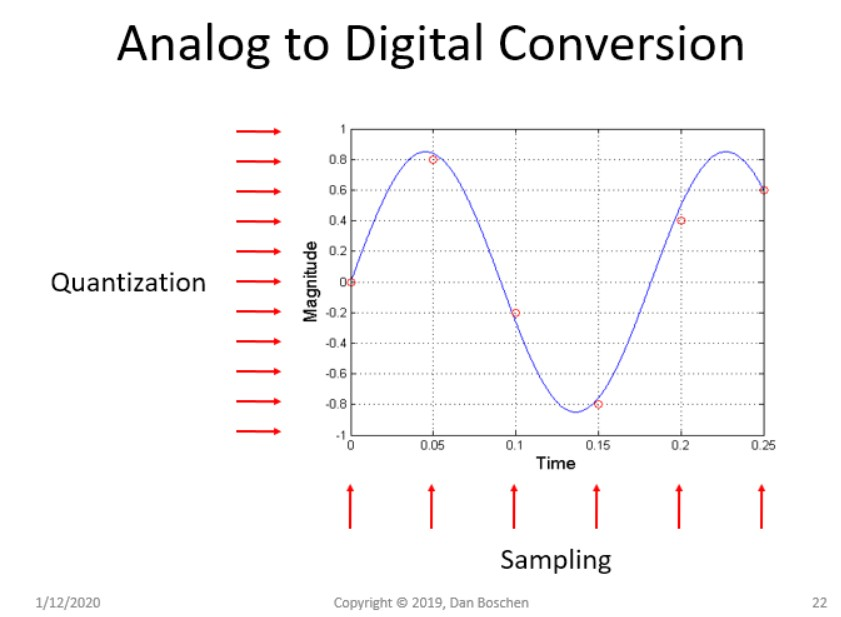
\includegraphics[width=0.8\textwidth]{figures/6-17.jpg}
        \caption{Échantillonnage}
    \label{fig:communication2}
\end{figure}
Les différences entre l'échantillonnage et la quantification sont:
\begin{itemize}
    \item Dans l'échantillonnage, \textbf{l'axe du temps} est discrétisé, tandis que dans la quantification, c'est \textbf{l'axe des y} (ou l'amplitude) qui est discrétisé.
    \item Dans le processus d'échantillonnage, \textbf{une seule valeur d'amplitude} est sélectionnée dans un intervalle de temps pour la représenter, tandis que dans la quantification, les valeurs représentant les intervalles de temps sont \textbf{arrondies} pour créer un ensemble fini de valeurs d'amplitude possibles.
    \item L'échantillonnage est effectué \textbf{avant} le processus de quantification.
\end{itemize}
\textbf{Aliasing}
À quelle fréquence devons-nous échantillonner ? Cela dépend de la rapidité avec laquelle le signal change (sa bande passante). Si nous n'échantillonnons pas assez vite, notre échantillon risque de ne pas être représentatif de la réalité.
Par exemple, deux signaux sinusoïdaux ayant des fréquences très différentes peuvent sembler identiques lorsqu’ils sont échantillonnés à basse fréquence.
\begin{figure}[H] % H force l'affichage ici
    \centering
    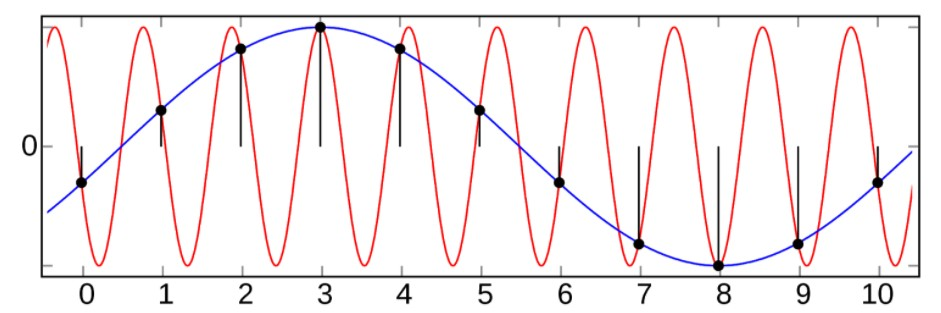
\includegraphics[width=0.8\textwidth]{figures/6-18.jpg}
    \caption{Graphique montrant l'aliasing d'une onde sinusoïdale f=0,9 par une onde sinusoïdale f=0,1 par échantillonnage à une période de T=1,0. CC BY-SA 3.0. Image de Mox Fyre.}
    \label{fig:communication2}
\end{figure}
Pour contrer l'aliasing, nous suivons le \textbf{théorème de Nyquist}, qui stipule que nous devons échantillonner au moins à :
\[
f_s = 2B
\]
où \( B \) est la bande passante.
\medskip
\noindent \textbf{Théorème de Nyquist}  
Le théorème d'échantillonnage de Nyquist-Shannon stipule :
\begin{quote}
    « Si une fonction \( x(t) \) ne contient aucune fréquence supérieure à \( B \) hertz, elle est complètement déterminée en donnant ses ordonnées à une série de points espacés de \( \frac{1}{2B} \) secondes. »
\end{quote}
Autrement dit, nous devons échantillonner au moins à :
\[
f_s = 2B
\]
(en pratique : \( f_s = 2.2B \)) où \( B \) est la limite de bande pour garantir une reconstruction parfaite du signal continu d'origine.  
Les scientifiques et les ingénieurs utilisent ce théorème pour décider de la fréquence d'échantillonnage d'un phénomène.  
Si le sujet scientifique qui nous intéresse se produit à \( B \) hertz, alors la charge utile doit échantillonner à \( 2B \) hertz.  
Si le mode dynamique d'attitude se produit à \( B \) hertz, alors l'IMU doit échantillonner à \( 2B \) hertz.
Si \( f_s - B > B \), nous pouvons alors appliquer un filtre passe-bas en \( B \) et reconstruire parfaitement le signal d'origine.
Si \( f_s - B < B \), il y a alors chevauchement (\textit{aliasing}) et nous ne pouvons pas reconstruire le signal.
\begin{figure}[H] % H force l'affichage ici
    \centering
    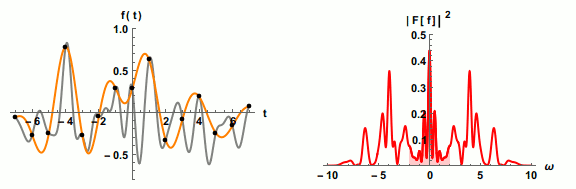
\includegraphics[width=0.8\textwidth]{figures/Nyquist_sampling.png}
    \caption{L'image de gauche montre une fonction (en gris/noir) échantillonnée et reconstruite (en doré) à des densités d'échantillonnage en constante augmentation, tandis que l'image de droite montre le spectre de fréquence de la fonction gris/noir, qui ne change pas. La fréquence la plus élevée du spectre est la moitié de la largeur du spectre entier. La largeur de l'ombrage rose en constante augmentation est égale à la fréquence d'échantillonnage. Lorsqu'elle englobe l'ensemble du spectre de fréquence, elle est deux fois plus grande que la fréquence la plus élevée, et c'est alors que la forme d'onde reconstruite correspond à celle échantillonnée. Image de Jacopo Bertolotti.}
    \label{fig:communication2}
\end{figure}
\textbf{Codage}
\begin{figure}[H] % H force l'affichage ici
    \centering
    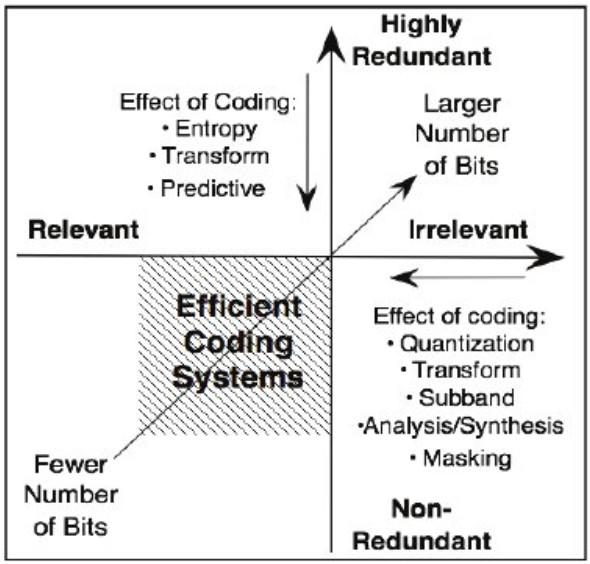
\includegraphics[width=0.8\textwidth]{figures/6-20.jpg}
    \caption{Réduction de la redondance et de la non-pertinence dans les schémas de codage. Kinsner, Witold. « L'entropie est-elle adaptée pour caractériser les données et les signaux en informatique cognitive ? » International Journal of Cognitive Informatics and Natural Intelligence (IJCINI) 1.2 (2007) : 34-57.}
    \label{fig:communication2}
\end{figure}
Le \textbf{codage source} et le \textbf{codage canal} sont deux types de codes différents utilisés dans les systèmes de communication numérique.  
Ils ont des objectifs \textbf{orthogonaux} :
\begin{itemize}
    \item L'objectif du \textbf{codage source} est la \textbf{compression des données} (diminution du débit de données).
    \item L'objectif du \textbf{codage de canal} est la \textbf{détection et correction des erreurs} (en augmentant le débit de données).
\end{itemize}
\begin{figure}[H] % H force l'affichage ici
    \centering
    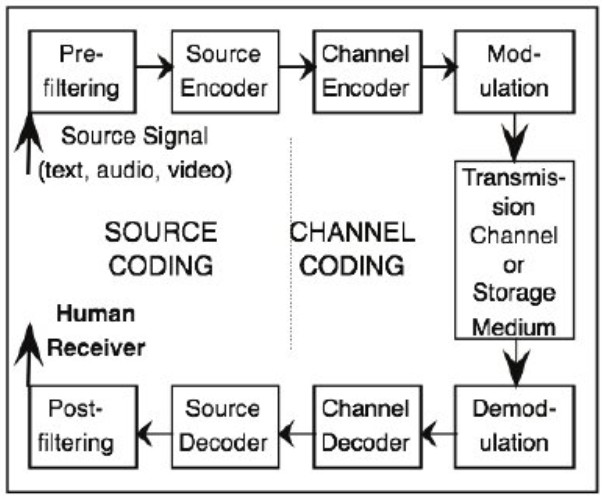
\includegraphics[width=0.8\textwidth]{figures/6-21.jpg}
    \caption{Codage conjoint source-canal-multimédia. Kinsner, Witold. « L'entropie est-elle adaptée pour caractériser les données et les signaux en informatique cognitive ? » Revue internationale d'informatique cognitive et d'intelligence naturelle (IJCINI) 1.2 (2007) : 34-57.}
    \label{fig:communication2}
\end{figure}
Le \textbf{codage source} vise à coder les données de manière plus efficace pour représenter l'information.  
Ce processus permet de \textbf{réduire la taille des données}.  
\textbf{Types de signaux et codage source} :
\begin{itemize}
    \item \textbf{Signaux analogiques} : Encodage des données analogiques dans un format binaire.
    \item \textbf{Signaux numériques} : Réduction de la taille des données sources numériques.
\end{itemize}
\textbf{Compression des données} :  
Il existe deux types de compression :
\begin{itemize}
    \item \textbf{Compression sans perte} :
    \begin{itemize}
        \item Permet une \textbf{reconstruction parfaite} du signal d'origine.
        \item Utilisée lorsque l'intégrité des données est essentielle.
        \item Ne permet qu'une \textbf{compression modérée} (ex. : 2:1 à 3:1) pour les images naturelles.
        \item Préconisée par de nombreux scientifiques dans les missions satellites.
        \item Exemples : fichiers \texttt{ZIP} et \texttt{PNG}.
    \end{itemize}
    \item \textbf{Compression avec perte} :
    \begin{itemize}
        \item Réduit davantage la taille des données en supprimant certaines informations.
        \item Exemples : formats \texttt{JPEG}, \texttt{MP3}, \texttt{MPEG}.
    \end{itemize}
\end{itemize}
\begin{figure}[H] % H force l'affichage ici
    \centering
    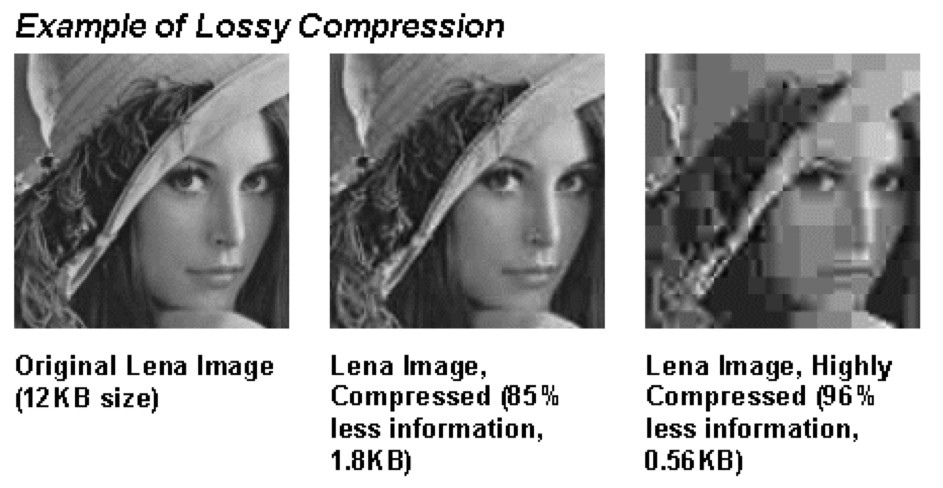
\includegraphics[width=0.8\textwidth]{figures/6-22.jpg}
    \caption{Exemple de compression avec perte. Image de Tyler Brown via WordPress.}
    \label{fig:communication2}
\end{figure}
Dans la compression avec perte, certaines informations sont perdues et une reconstruction parfaite n'est pas possible, mais en général, une réduction beaucoup plus importante du débit binaire est obtenue. Elle est utilisée lorsque la réduction du débit binaire est très importante et que l'intégrité n'est pas critique. Le codage source avec perte peut atteindre une compression beaucoup plus importante (par exemple 20:1 – 40:1) pour les images naturelles. Les exemples incluent les fichiers jpg (images) et mp3 (audio).
\begin{figure}[H] % H force l'affichage ici
    \centering
    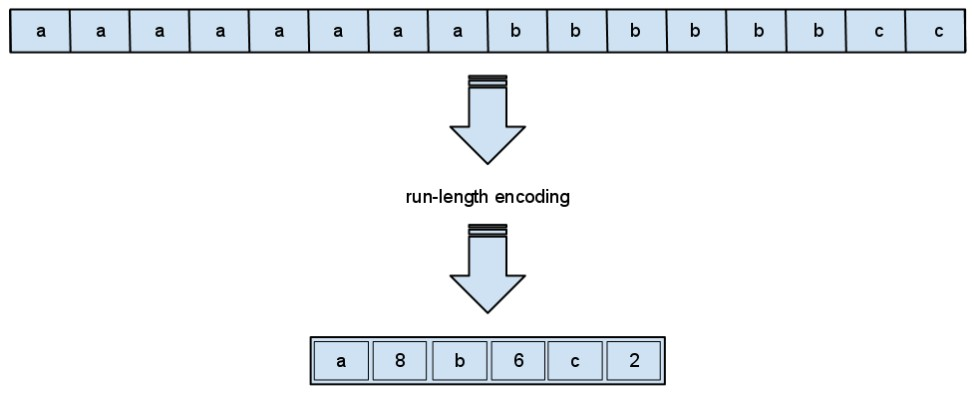
\includegraphics[width=0.8\textwidth]{figures/6-23.jpg}
    \caption{Exemple de codage de longueur d'exécution avec données originales et représentation compressée. Image du professeur GR Sinha.}
    \label{fig:communication2}
\end{figure}
Les méthodes de \textbf{compression sans perte} exploitent généralement la structure de l'information.  
Un exemple d'algorithme de compression sans perte est le \textbf{codage de longueur d'exécution} (\textit{Run-Length Encoding}, RLE). Ce type de codage est particulièrement avantageux lorsque les données contiennent des séquences répétées de la même valeur, apparaissant dans de nombreux éléments de données consécutifs.  
Dans ce cas :
\begin{itemize}
    \item Il existe des \textbf{chaînes relativement longues} de 0 ou de 1 (changements peu fréquents).
    \item Certaines \textbf{combinaisons de bits sont plus probables} que d'autres.
\end{itemize}
Dans le codage RLE, les séries de données sont stockées sous la forme d'une \textbf{valeur unique suivie du nombre de répétitions}, plutôt que d'enregistrer la série d'origine.  
\medskip
\textbf{Exemple :}  
\[
[1,0,0,0,0,0,0,0,0,0,0,1,1,\dots] \rightarrow [1,10,2]
\]
Notez que cela n'est utile que s'il existe de nombreuses longues séries de données (par exemple, de simples images en noir et blanc avec principalement du blanc).
Un autre type de compression sans perte est le codage Huffman, où si certains symboles sont plus probables que d'autres, nous pouvons utiliser moins de bits pour coder les combinaisons les plus probables. Cela entraînera des réductions du débit binaire sans perte d'informations.
\begin{figure}[H] % H force l'affichage ici
    \centering
    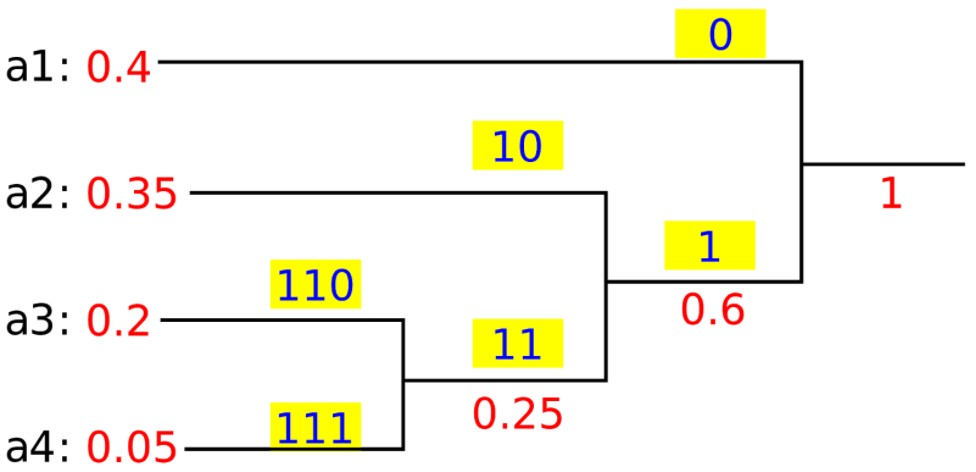
\includegraphics[width=0.8\textwidth]{figures/6-24.jpg}
    \caption{Une source génère 4 symboles différents}
    \label{fig:communication2}
\end{figure}
Le code Huffman final est présenté dans le tableau suivant :
\begin{center}
    \begin{tabular}{|c|c|}
        \hline
        \textbf{Symbole} & \textbf{Code} \\
        \hline
        $a_1$ & 1 \\
        $a_2$ & 10 \\
        $a_3$ & 110 \\
        $a_4$ & 111 \\
        \hline
    \end{tabular}
\end{center}
La manière standard de représenter un signal constitué de 4 symboles est d'utiliser 2 bits/symbole, mais l'entropie de la source est de 1,74 bits/symbole. Si ce code de Huffman est utilisé pour représenter le signal, alors la longueur moyenne est abaissée à 1,85 bits/symbole ; on est encore loin de la limite théorique car les probabilités des symboles sont différentes des puissances négatives de deux.
L'algorithme de \textbf{codage de Huffman} est le suivant :
\begin{itemize}
    \item Attribuez \textbf{0} au symbole le plus probable, les autres commencent par \textbf{1}.
    \item Attribuez \textbf{10} au symbole le plus probable parmi les restants, les autres commencent par \textbf{11}.
    \item Continuez ce processus récursivement jusqu'à ce que tous les symboles soient codés.
\end{itemize}
\textbf{Codes préfixes :} comment savoir quand commence un symbole s'il est de longueur variable ?  
Les codes préfixes (comme Huffman) ne nécessitent aucun marqueur malgré leur longueur variable, car ils sont conçus de manière à éviter toute confusion possible.
\textbf{Codage des canaux :}  
Le codage des canaux a pour but de garantir que les données reçues sont identiques à celles envoyées.  
\textit{« Les liaisons sans fil souffrent d’interférences et d’évanouissements qui provoquent des erreurs. Pour y remédier, l’émetteur ajoute des informations supplémentaires avant l’envoi des données. Ensuite, du côté du récepteur, des codes complexes nécessitant des algorithmes sophistiqués décodent ces informations et récupèrent les données d’origine. »}  
La détection et la correction des erreurs reposent sur une idée clé : ajouter des bits de redondance de manière stratégique pour éviter les erreurs.
\textbf{Comment détecter une erreur ?}  
Imaginons que nous ajoutions un bit de parité à la fin de chaque bit $N$ de sorte que la somme de tous les bits, y compris le bit de parité, soit toujours égale à 0. Nous pouvons alors détecter une erreur :
\begin{align*}
01010101 &\quad \text{→ somme = 0, OK aucune erreur. (ou il pourrait y avoir 2 erreurs !)} \\
11101100 &\quad \text{→ somme = 1, NOK. Il y a une erreur (mais je ne peux pas la corriger)}
\end{align*}
\textbf{Comment corriger une erreur ?}  
Imaginons que nous transmettions simplement chaque bit 3 fois. Il y a alors deux symboles possibles : 000 et 111. Nous disons que le code a une distance de 3 car 3 bits doivent changer pour transformer un symbole valide en un autre.
\begin{align*}
100, 010, 001 &\quad \text{→ corrigé à 000} \\
110, 101, 011 &\quad \text{→ corrigé à 111}
\end{align*}
\begin{figure}[H] % H force l'affichage ici
    \centering
    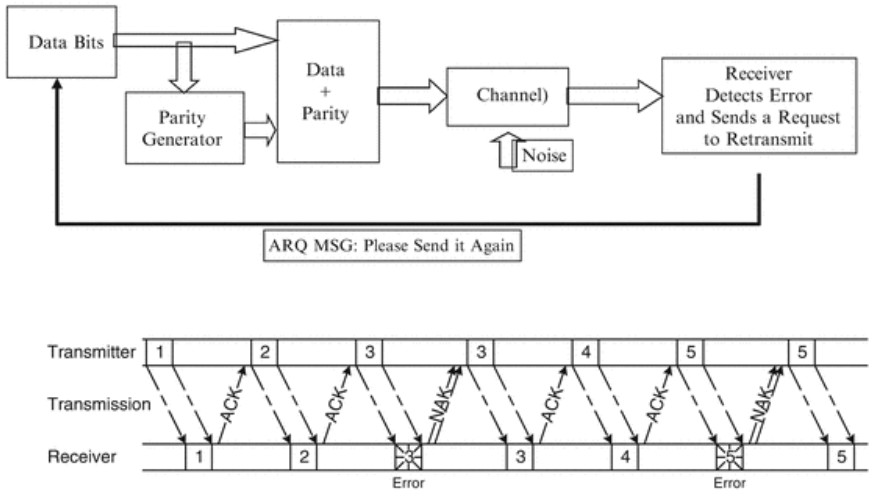
\includegraphics[width=0.8\textwidth]{figures/6-25.jpg}
    \caption{Boucle de codage de canal où la parité est non seulement ajoutée mais où le récepteur vérifie si une erreur a été détectée, un message de demande de répétition automatique (ARQ) est envoyé. Image de Springer Link.}
    \label{fig:communication2}
\end{figure}
Si nous détectons une erreur, nous pouvons demander une retransmission. On parle alors parfois de correction d'erreur en amont. Cela s'oppose à la correction d'erreur en aval (FEC) dans laquelle la correction d'erreur est intégrée à la transmission. 
Propriétés des codes FEC :
\begin{itemize}
    \item \textbf{Distance} : nombre minimum de bits nécessaires pour effectuer une transformation entre deux symboles valides.
    \item \textbf{Nombre d'erreurs détectées/corrigées}.
    \item \textbf{Taux} : Nombre de bits de données / Nombre total de bits  
          \( \rho = \frac{n - r}{n} \)
    \item \textbf{Gain de code} : Gain en dB dans l'équation de budget de liaison pour un BER (taux d'erreur binaire) égal.
\end{itemize}
Deux principaux types de codes correcteurs d’erreurs :
\begin{itemize}
    \item \textbf{Codes de bloc} :
          \begin{itemize}
              \item Codes de Hamming
              \item Reed-Salomon
          \end{itemize}
    \item \textbf{Codes convolutifs} :
          \begin{itemize}
              \item Viterbi
          \end{itemize}
\end{itemize}
Les codes de Hamming sont une famille de codes correcteurs d'erreurs linéaires. Le code de Hamming est le code Hadamard raccourci. Les codes de Hamming peuvent détecter des erreurs allant jusqu'à deux bits ou corriger des erreurs d'un bit sans détecter d'erreurs non corrigées. En revanche, le code de parité simple ne peut pas corriger les erreurs et ne peut détecter qu'un nombre impair de bits erronés. Les codes de Hamming sont des \textbf{codes parfaits}, c'est-à-dire qu'ils atteignent le taux le plus élevé possible pour des codes avec leur longueur de bloc et leur distance minimale de trois.
\begin{figure}[H] % H force l'affichage ici
    \centering
    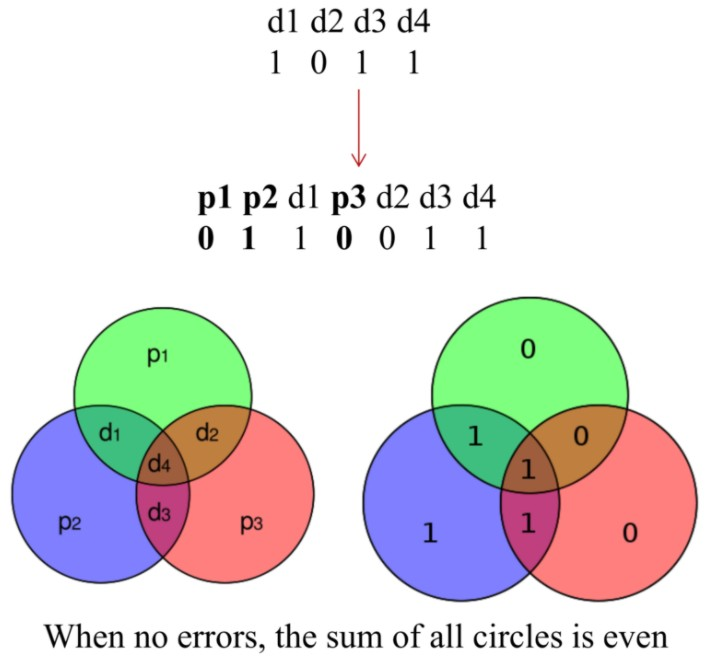
\includegraphics[width=0.8\textwidth]{figures/6-26.jpg}
    \caption{Le code de Hamming(7,4) (avec r = 3). Représentation graphique des quatre bits de données et des trois bits de parité et des bits de parité qui s'appliquent à quels bits de données. CC BY-SA 3.0. Image de C. Burnett.}
    \label{fig:communication2}
\end{figure}
Tous les codes de Hamming ont une distance de 3, peuvent détecter 2 erreurs et en corriger 1.  
Les longueurs des messages des codes de Hamming sont exprimées en $(2^r -1 , 2^r - r - 1)$ : (bits totaux, bits de données). Par exemple :
\begin{itemize}
    \item \textbf{Hamming(3,1)} est un message avec triple répétition.
    \item \textbf{Hamming(7,4)} est un message qui ajoute 3 bits de redondance à chaque 4 bits de données.
\end{itemize}
Le taux d'un code de bloc est défini comme le rapport entre la longueur de son message et la longueur de son bloc.  
Pour ce code de bloc, le taux est de $ \frac{4}{7} $.
Les bits de parité sont ajoutés aux positions $ 1, 2, 4, 8, \dots $. Les autres sont des bits de données.  
Chaque bit de parité couvre un sous-ensemble différent de bits :  
Le bit de parité 1 couvre toutes les positions de bits dont le bit le moins significatif est défini (1, 3, 5, …).
\begin{figure}[H] % H force l'affichage ici
    \centering
    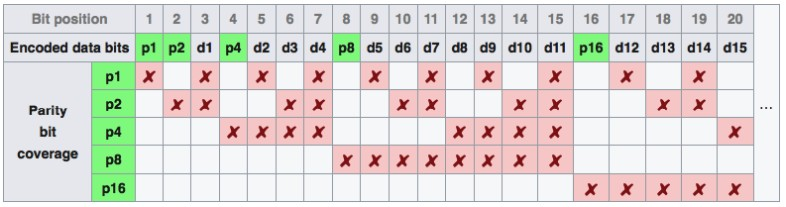
\includegraphics[width=0.8\textwidth]{figures/6-27.jpg}
    \caption{L'algorithme général suivant génère un code de correction d'erreur unique (SEC) pour n'importe quel nombre de bits. Seuls 20 bits codés (5 de parité, 15 de données) sont représentés, mais le modèle se poursuit indéfiniment. L'élément clé des codes de Hamming qui peut être vu à partir d'une inspection visuelle est que chaque bit donné est inclus dans un ensemble unique de bits de parité. Pour vérifier les erreurs, vérifiez tous les bits de parité. Image par Artillar. }
    \label{fig:communication2}
\end{figure}
Intuitivement, 1 erreur peut être corrigée grâce à la distance de 3 entre les symboles valides. Comme chaque bit est affecté à un ensemble unique de bits de parité, nous pouvons identifier quel bit est erroné en identifiant le bit pour lequel tous les bits de parité sont erronés d2. La position du bit erroné est égale à la somme des positions de tous les bits de parité erronés : 1(p1) + 4(p3) = 5 (d2).
\begin{figure}[H] % H force l'affichage ici
    \centering
    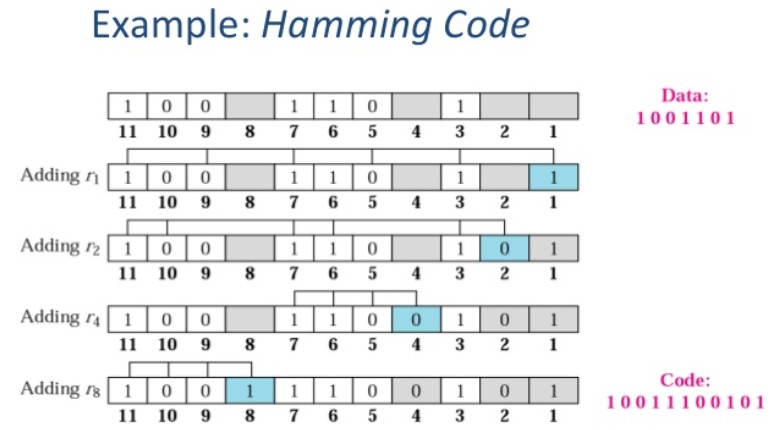
\includegraphics[width=0.8\textwidth]{figures/6-28.jpg}
    \caption{Exemple de code de Hamming. CC-BY SA 4. Image par Artillar.}
    \label{fig:communication2}
\end{figure}
Un autre algorithme de codage de canal est appelé \textbf{code de correction d'erreurs Reed-Solomon}.  
Contrairement aux algorithmes basés sur les bits, l'algorithme Reed-Solomon opère sur des \textit{symboles}, généralement constitués de blocs de 8 bits.  

Ce type de codage est particulièrement efficace pour la correction des \textit{erreurs en rafale}, car plusieurs bits erronés peuvent être considérés comme un seul symbole erroné.  
Le code Reed-Solomon convertit $k$ symboles de données en $n > k$ symboles redondants à l'aide de polynômes, permettant ainsi de détecter et de corriger un certain nombre d'erreurs.
Codage Reed-Solomon pour la tolérance aux pannes. Accélérez le codage Reed-Solomon pour la tolérance aux pannes dans un système de type RAID par Shuai Yuan.
\begin{figure}[H] % H force l'affichage ici
    \centering
    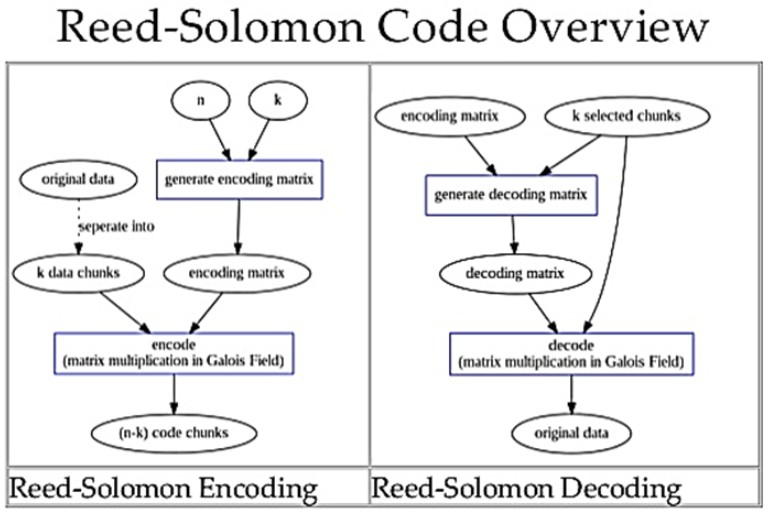
\includegraphics[width=0.8\textwidth]{figures/6-29.jpg}
    
    \caption{Codage Reed-Solomon pour la tolérance aux pannes. Accélérez le codage Reed-Solomon pour la tolérance aux pannes dans un système de type RAID par Shuai Yuan.}
    \label{fig:communication2}
\end{figure}
\textbf{Codage : deux étapes}
\begin{itemize}
    \item Interpréter le message $x = [x_1, x_2, \dots, x_k]$ comme les coefficients d'un polynôme de degré $k - 1$ :
    \[
    p_x(a) = \sum_{i=1}^{k} x_i a^{i-1}
    \]
    
    \item Évaluer le polynôme en $n$ points différents :
    \[
    C(x) = [p_x(a_1), p_x(a_2), \dots, p_x(a_n)]
    \]
\end{itemize}
\textbf{Décodage :} Basé sur la régression (trouver un polynôme qui passe par les $n$ points).
Par exemple, Reed-Solomon (255,223) ajoute 32 symboles redondants pour 223 symboles de données. Il peut détecter 32 erreurs et en corriger 16. Read-Solomon est utilisé de manière exhaustive dans l'espace, notamment en concaténation avec des codes convolutifs (par exemple Voyager, Meteosat, Timed).
\begin{figure}[H] % H force l'affichage ici
    \centering
    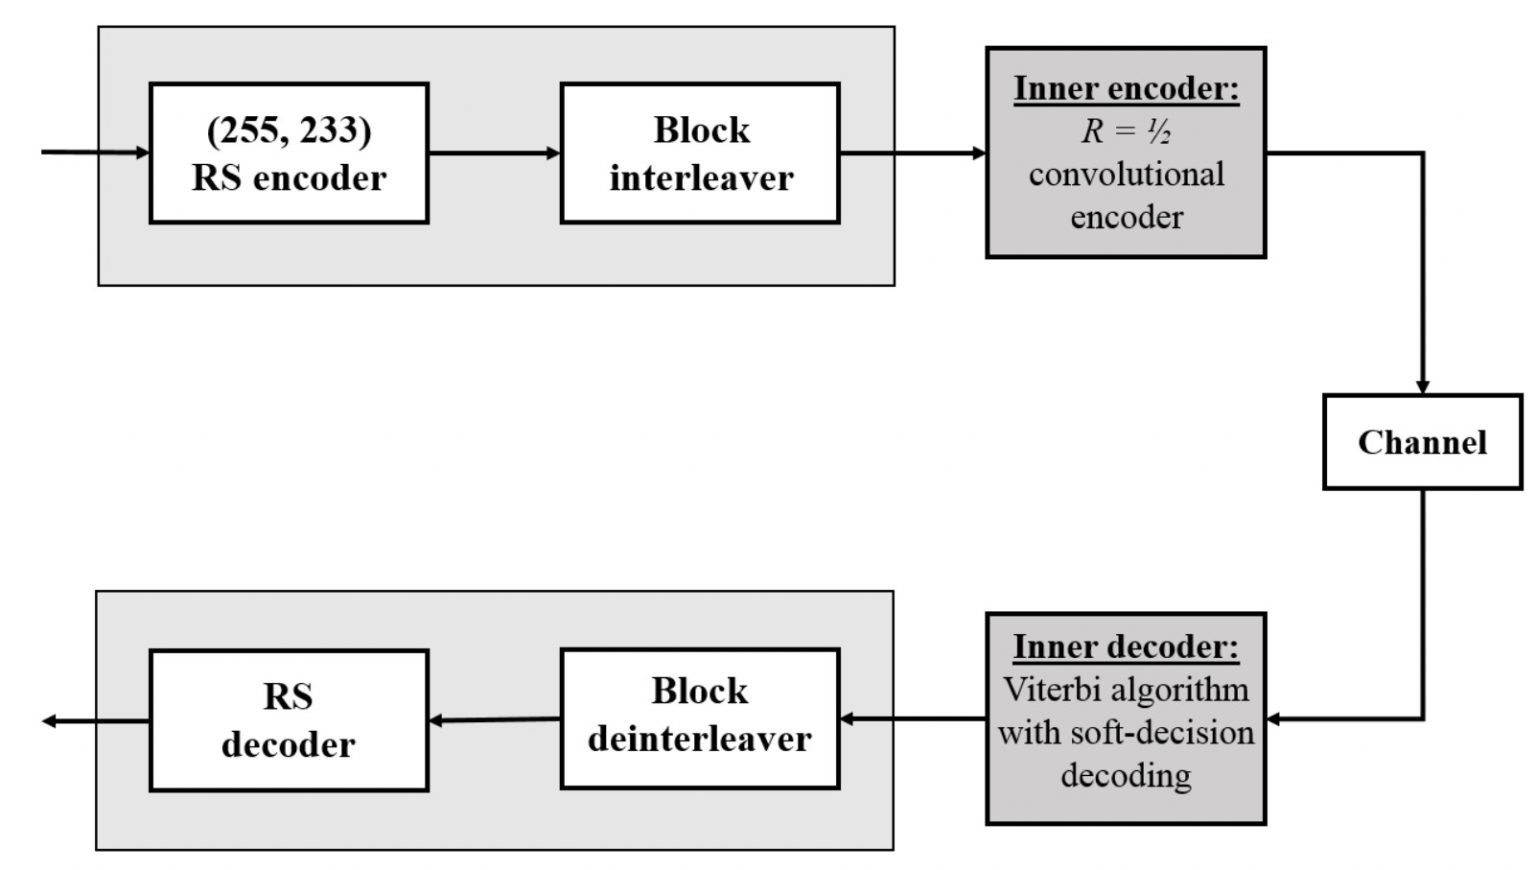
\includegraphics[width=0.8\textwidth]{figures/6-30.jpg}
    \caption{Système de codage concaténé en espace profond. Notation : RS(255, 223) + CC (« longueur de contrainte » = 7, taux de codage = 1/2). CC BY-SA 4.0. Image de Kirlf.}
    \label{fig:communication2}
\end{figure}
\begin{figure}[H] % H force l'affichage ici
    \centering
    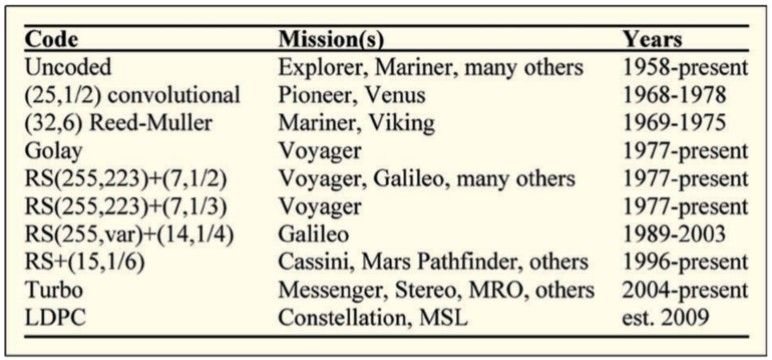
\includegraphics[width=0.8\textwidth]{figures/6-31.jpg}
    \caption{Codes Used by NASA Missions Andrews, Kenneth S., et al. “The development of turbo and LDPC codes for deep-space applications.” Proceedings of the IEEE 95.11 (2007): 2142-2156. Image by IEEE Explore.}
    \label{fig:communication2}
\end{figure}
\textbf{Modulations}
\textbf{Lectures suggérées :} 
\href{https://deepspace.jpl.nasa.gov/dsndocs/810-005/208/208B.pdf}{\textit{Système de télémétrie DSN, décodage des données}}
Les informations entre le satellite et la station terrestre sont transmises en modifiant certaines propriétés (amplitude, fréquence ou phase) d'un signal porteur haute fréquence $c(t)$ de manière à coder les informations dans le message $m(t)$.  
C'est ce qu'on appelle la \textbf{modulation}. Il existe un schéma de modulation pour les signaux analogiques et numériques que nous examinerons dans cette section.
\vspace{0.5cm}
\textbf{Pourquoi avons-nous besoin de modulation ? Pourquoi ne pouvons-nous pas simplement transmettre notre train d'impulsions (bits) ?}
\begin{itemize}
    \item Ce sont des signaux de très basse fréquence.
    \item Les signaux basse fréquence nécessiteraient des antennes extrêmement grandes.
    \item Les signaux basse fréquence ont d'énormes pertes atmosphériques.
\end{itemize}
\vspace{0.5cm}
Les modulations sont basées sur la modification de la fonction sinusoïdale.  
Les trois paramètres d'une sinusoïde qui peuvent être modifiés sont :
\begin{itemize}
    \item \textbf{Amplitude}
    \item \textbf{Fréquence}
    \item \textbf{Phase}
\end{itemize}
\textbf{Modulation d'amplitude (AM)}
\begin{figure}[H] % H force l'affichage ici
    \centering
    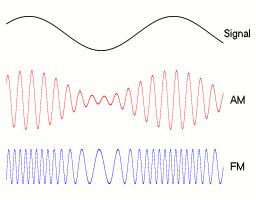
\includegraphics[width=0.8\textwidth]{figures/Amfm3-en-de-0003.jpg}
    \caption{Diagramme représentant la différence entre les ondes radio modulées en amplitude et en fréquence. CC BY-SA 2.5. Image de Berserkerus. }
    \label{fig:communication2}
\end{figure}
« La modulation d'amplitude (AM) est une technique de modulation utilisée dans les communications électroniques, le plus souvent pour transmettre des messages avec une onde porteuse radio . Dans la modulation d'amplitude, l' amplitude (intensité du signal) de l'onde porteuse varie proportionnellement à celle du signal du message » . Cet algorithme modulaire est facile à mettre en œuvre mais présente de faibles performances en matière de bruit.
\begin{figure}[H] % H force l'affichage ici
    \centering
    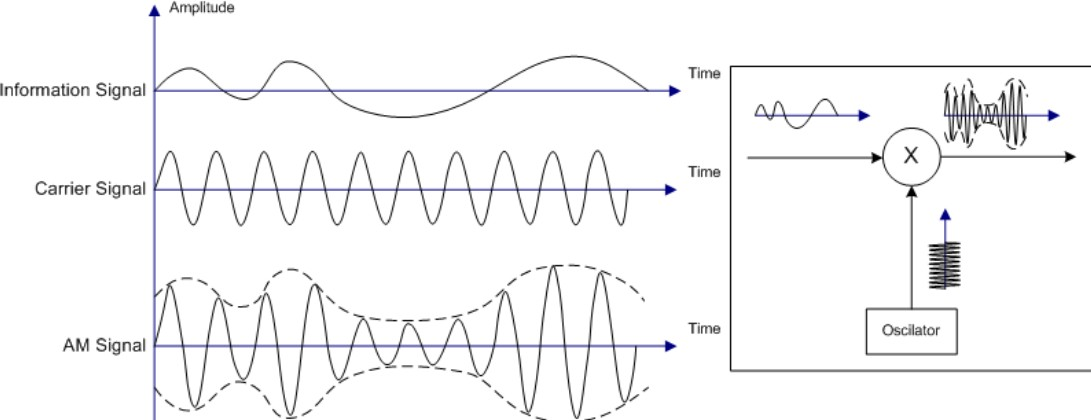
\includegraphics[width=0.8\textwidth]{figures/6-32.jpg}
    \caption{L'illustration de la modulation d'amplitude (AM) montre une comparaison entre un signal d'information, un signal porteur et un signal AM. CC BY-SA 3.0. Image par Ivan }
    \label{fig:communication2}
\end{figure}
Supposons que le signal porteur à la fréquence radio sous licence ait la forme :  
\[
c(t) = A_c \cos(\omega_c t).
\]
Le signal analogique est $m(t)$ avec une bande passante $B$, généralement $B \ll \omega_c$.  
Des exemples de signaux analogiques sont :
\begin{itemize}
    \item L'audio autour de $4$ kHz.
    \item La vidéo à $4$ MHz.
\end{itemize}
Le signal modulé en amplitude à la fréquence radio sous licence est donné par :
\[
s_{AM} (t) = A_c (1 + m(t)) \cos(\omega_c t).
\]
\begin{figure}[H] % H force l'affichage ici
    \centering
    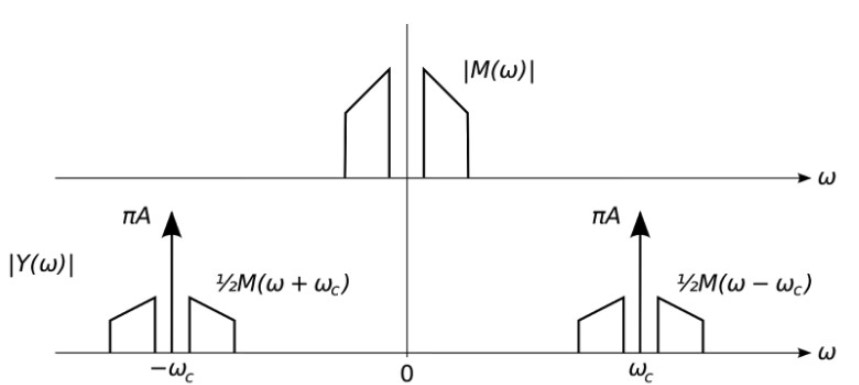
\includegraphics[width=0.8\textwidth]{figures/6-121.jpg}
  \caption{Spectres bilatéraux des signaux en bande de base et AM. CC BY-SA 3.0. Image de Splash. }
    \label{fig:communication2}
\end{figure}
\textbf{La modulation d'amplitude nécessite :}
\begin{itemize}
    \item Un oscillateur local pour générer le signal porteur haute fréquence.
    \item Un mixeur pour mélanger (multiplier) les deux signaux.
    \item Un amplificateur.
\end{itemize}
\begin{figure}[H] % H force l'affichage ici
    \centering
    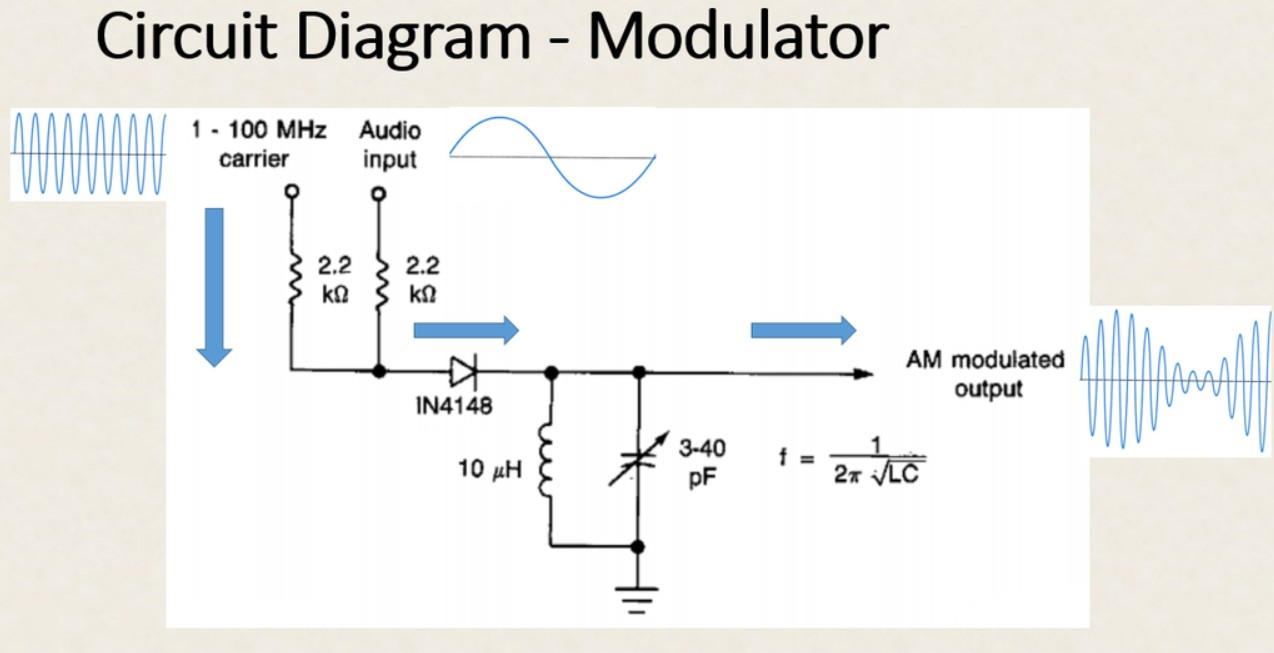
\includegraphics[width=0.8\textwidth]{figures/6-34.jpg}
    \caption{Ce modulateur à diode simple fournit d'excellents résultats lorsqu'il est utilisé pour une modulation à pourcentage élevé à de faibles niveaux de signal. Image par Instructables.}
    \label{fig:communication2}
\end{figure}
\textbf{La démodulation du signal nécessite :}
\begin{itemize}
    \item Un oscillateur local pour générer un proxy du signal porteur.
    \item Un mixeur pour multiplier.
    \item Un filtre passe-bas pour ne conserver que la partie basse fréquence du signal reçu.
    \item Une diode pour supprimer la partie DC.
\end{itemize}
\begin{figure}[H] % H force l'affichage ici
    \centering
    \includegraphics[width=0.8\textwidth]{figures/6-35.jpg}
    \caption{La combinaison du condensateur C et de la résistance R se comporte comme un filtre passe-bas. Le signal d'entrée contient à la fois le message d'origine et l'onde porteuse, le condensateur aidant à filtrer les ondes porteuses RF. Le condensateur se charge pendant le front montant et se décharge à travers la résistance R pendant le front descendant. Ainsi, le condensateur permet de donner une enveloppe de l'entrée en sortie. Image par Instructables.}
    \label{fig:communication2}
\end{figure}
\textbf{Modulation de fréquence (FM)}
\begin{figure}[H] % H force l'affichage ici
    \centering
    \includegraphics[width=0.8\textwidth]{figures/6-36.jpg}
    \caption{La modulation d'un signal analogique en une porteuse analogique en utilisant la modulation de fréquence (FM). CC BY-SA 4.0. Image de Michel Bakni.}
    \label{fig:communication2}
\end{figure}
« La modulation de fréquence (FM) est le codage d' informations dans une onde porteuse en faisant varier la fréquence instantanée de l'onde. Cette technologie est utilisée dans les télécommunications , la radiodiffusion , le traitement du signal et l'informatique . Dans la transmission radio, l'un des avantages de la modulation de fréquence est qu'elle présente un rapport signal/bruit plus élevé et qu'elle rejette donc mieux les interférences radioélectriques qu'un signal de modulation d'amplitude (AM) de puissance égale » 
\begin{figure}[H] % H force l'affichage ici
    \centering
    \includegraphics[width=0.8\textwidth]{figures/6-37.jpg}
    \caption{Spectre de fréquence et courbe en cascade d'une porteuse de 146,52 MHz, modulée en fréquence par une sinusoïde de 1 000 Hz. L'indice de modulation a été ajusté à environ 2,4, de sorte que la fréquence porteuse a une faible amplitude. Plusieurs bandes latérales fortes sont apparentes ; en principe, un nombre infini de bandes latérales sont produites en FM, mais les bandes latérales d'ordre supérieur sont d'une amplitude négligeable. CC BY-SA 4.0. Image de Wtshymanski.}
    \label{fig:communication2}
\end{figure}
Supposons à nouveau un signal porteur de la forme :  
\[
c(t) = A_c \cos(\omega_c t).
\]
Le signal analogique que nous essayons de convertir est de la forme $m(t)$ avec une bande passante $B$, typiquement $B \ll \omega_c$.  
Le signal modulé en fréquence prend la forme :
\[
s_{FM}(t) = A_c \cos\left( \int_0^t (\omega_c + f_{\Delta} m (\tau)) \, d\tau \right) 
= A_c \cos\left(\omega_c t + f_{\Delta} \int_0^t m (\tau) \, d\tau \right).
\]
\textbf{Caractéristiques du spectre et de la modulation FM :}
\begin{itemize}
    \item Le spectre d'un signal FM est difficile à calculer analytiquement, même pour des messages simples.
    \item La modulation et la démodulation FM sont similaires à l'AM en principe, mais nécessitent des intégrateurs et des différenciateurs.
    \item La modulation de fréquence nécessite une boucle de verrouillage de fréquence, qui peut être mise en œuvre avec des résistances, des condensateurs et des amplificateurs opérationnels, par exemple.
\end{itemize}
\textbf{Types de modulation FM :}
\begin{itemize}
    \item \textbf{Modulation FM directe} : obtenue en alimentant directement le message dans l'entrée d'un oscillateur contrôlé en tension.
    \item \textbf{Modulation FM indirecte} :
    \begin{itemize}
        \item Le signal de message est intégré pour générer un signal modulé en phase.
        \item Ce signal est utilisé pour moduler un oscillateur contrôlé par cristal.
        \item Le résultat est passé à travers un multiplicateur de fréquence pour produire un signal FM.
        \item Une FM à bande étroite est générée en premier, puis transformée en FM à large bande.
        \item Cette technique est connue sous le nom de \textbf{modulation FM indirecte}.
    \end{itemize}
\end{itemize}
\textbf{Méthodes de démodulation FM :}
\begin{itemize}
    \item Une méthode courante pour récupérer le signal d'information consiste à utiliser un \textbf{discriminateur Foster-Seeley} ou un \textbf{détecteur de rapport}.
    \item Une \textbf{boucle à verrouillage de phase (PLL)} peut être utilisée comme démodulateur FM.
    \item La \textbf{détection de pente} démodule un signal FM en utilisant un circuit accordé dont la fréquence de résonance est légèrement décalée par rapport à la porteuse.  
    \begin{itemize}
        \item Lorsque la fréquence monte et descend, le circuit accordé fournit une amplitude de réponse variable.
        \item Cette variation convertit la FM en AM.
    \end{itemize}
\end{itemize}
\begin{figure}[H] % H force l'affichage ici
    \centering
    \includegraphics[width=0.8\textwidth]{figures/6-38.jpg}
    \caption{Modulateur de fréquence à boucle à verrouillage de phase (PLL FM). Le signal FM d'entrée et la sortie de l'oscillateur contrôlé en tension (VCO) sont appliqués au circuit détecteur de phase. La sortie du détecteur de phase est filtrée à l'aide d'un filtre passe-bas, de l'amplificateur, puis utilisée pour contrôler le VCO. Lorsqu'il n'y a pas de modulation de porteuse et que le signal FM d'entrée est au centre de la bande passante, la tension de ligne de réglage du VCO sera à la position centrale. Lorsqu'une déviation de la fréquence porteuse se produit (ce qui signifie qu'une modulation se produit), la fréquence du VCO suit le signal d'entrée afin de maintenir la boucle verrouillée. En conséquence, la tension de ligne de réglage du VCO varie et cette variation est proportionnelle à la modulation effectuée sur l'onde porteuse FM. La variation de tension est filtrée et amplifiée afin d'obtenir le signal démodulé. Image de Circuits Today.}
    \label{fig:communication2}
\end{figure}
\textbf{Modulation de phase}
\textbf{Modulation de phase (PM) :}
\begin{itemize}
    \item La modulation de phase (PM) est un modèle de modulation permettant de conditionner les signaux de communication en vue de leur transmission.
    \item Elle code un signal de message sous forme de variations de la phase instantanée d'une onde porteuse.
    \item La modulation de phase est l'une des deux principales formes de \textbf{modulation d'angle}, avec la modulation de fréquence (FM).
    \item La phase d'un signal porteur est modulée pour suivre le niveau de signal changeant (amplitude) du signal de message.
    \item L'amplitude de crête et la fréquence du signal porteur sont maintenues constantes, mais lorsque l'amplitude du signal de message change, la phase du signal porteur change en conséquence.
    \item La modulation de phase est largement utilisée pour transmettre des ondes radio.
    \item Elle fait partie intégrante de nombreux schémas de codage de transmission numérique, sous-tendant un large éventail de technologies, telles que :
    \begin{itemize}
        \item \textbf{Wi-Fi},
        \item \textbf{GSM},
        \item \textbf{Télévision par satellite}.
    \end{itemize}
\end{itemize}
\begin{figure}[H] % H force l'affichage ici
    \centering
    \includegraphics[width=0.8\textwidth]{figures/500px-Phase-modulation.png}
    \caption{L'onde modulante (bleue) module l'onde porteuse (rouge), ce qui donne le signal PM (vert). Image de Potasmic.}
    \label{fig:communication2}
\end{figure}
Supposons à nouveau un signal porteur de la forme :  
\[
c(t) = A_c \cos(\omega_c t + \phi_c).
\]
Le signal analogique que nous essayons de convertir est de la forme $m(t)$ avec une bande passante $B$, typiquement $B \ll \omega_c$.  
Le signal modulé en phase prend la forme :
\[
s_{PM}(t) = A_c \cos(\omega_c t + m(t) + \phi_c).
\]
\begin{figure}[H] % H force l'affichage ici
    \centering
    \includegraphics[width=0.8\textwidth]{figures/6-39.jpg}
    \caption{Schéma de principe du modulateur de phase. Image de McGraw-Hill Companies.}
    \label{fig:communication2}
\end{figure}
\textbf{Système de contrôle à boucle de verrouillage de phase (PLL) :}

\begin{itemize}
    \item La modulation de phase nécessite un \textbf{système de contrôle à boucle de verrouillage de phase} (PLL).
    \item Il existe plusieurs types de PLL, le plus simple étant un circuit électronique comprenant :
    \begin{itemize}
        \item Un \textbf{oscillateur à fréquence variable}.
        \item Un \textbf{détecteur de phase} dans une boucle de rétroaction.
    \end{itemize}
    \item Fonctionnement :
    \begin{itemize}
        \item L'oscillateur génère un signal périodique.
        \item Le détecteur de phase compare la phase du signal généré à celle du signal périodique d'entrée.
        \item Le détecteur ajuste l'oscillateur pour maintenir les phases correspondantes.
    \end{itemize}
\end{itemize}

\textbf{Modulation numérique :}

\begin{itemize}
    \item Contrairement à la modulation analogique, la \textbf{modulation numérique} transforme un signal binaire.
    \item Le signal porteur reste un signal analogique.
    \item La modulation numérique utilise un \textbf{nombre fini de signaux analogiques} (impulsions) pour représenter des parties d'un message numérique.
    \item Exemple :
    \begin{itemize}
        \item Le code \textbf{00} peut être représenté par : 
        \[
        A_c \cos(\omega_c t).
        \]
        \item Nous pouvons encoder un \textbf{0} comme :
        \[
        \cos(\omega_0 t),
        \]
        \item et un \textbf{1} comme :
        \[
        \cos(\omega_1 t).
        \]
    \end{itemize}
    \item Ce type de modulation est appelé \textbf{modulation par déplacement de fréquence} (FSK - Frequency Shift Keying).
    \item En \textbf{FSK binaire}, il n'y a que deux fréquences distinctes :
    \begin{itemize}
        \item \textbf{0} est transmis à la fréquence $f_0$.
        \item \textbf{1} est transmis à la fréquence $f_1$.
    \end{itemize}
    \item Nous pouvons aussi avoir des variantes comme :
    \begin{itemize}
        \item \textbf{4-FSK} : utilise 4 fréquences distinctes :
        \begin{itemize}
            \item \textbf{00} : $f_{00}$,
            \item \textbf{01} : $f_{01}$,
            \item \textbf{10} : $f_{10}$,
            \item \textbf{11} : $f_{11}$.
        \end{itemize}
        \item \textbf{8-FSK} : utilise 8 fréquences différentes, etc.
    \end{itemize}
\end{itemize}

\begin{figure}[H] % H force l'affichage ici
    \centering
    \includegraphics[width=0.8\textwidth]{figures/6-40.png}
    \caption{Exemple de FSK binaire. CC BY-SA 3.0. Image de K.Tims.}
    \label{fig:communication2}
\end{figure}
\textbf{Modulation numérique par déplacement d'amplitude (ASK) :}
\begin{itemize}
    \item Une autre méthode de modulation consiste à encoder :
    \begin{itemize}
        \item Un \textbf{0} comme :
        \[
        A_0 \cos(\omega_c t),
        \]
        \item Un \textbf{1} comme :
        \[
        A_1 \cos(\omega_c t).
        \]
    \end{itemize}
    \item Cette technique est appelée \textbf{modulation par déplacement d'amplitude} (ASK - Amplitude Shift Keying).
    \item Dans cette modulation, les \textbf{symboles correspondent à différentes amplitudes}.
    \item En \textbf{ASK binaire}, nous utilisons deux amplitudes distinctes :
    \begin{itemize}
        \item \textbf{0} est représenté par l'amplitude $A_0$,
        \item \textbf{1} est représenté par l'amplitude $A_1$.
    \end{itemize}
    \item Généralement, $A_0 = 0$.
    \item Nous pouvons également avoir des variantes comme :
    \begin{itemize}
        \item \textbf{4-ASK}, \textbf{8-ASK}, etc.
    \end{itemize}
    \item De même, pour la \textbf{4-ASK}, différentes amplitudes sont utilisées :
    \begin{itemize}
        \item \textbf{00} : $A_{00}$,
        \item \textbf{01} : $A_{01}$,
        \item \textbf{10} : $A_{10}$,
        \item \textbf{11} : $A_{11}$.
    \end{itemize}
\end{itemize}
\begin{figure}[H] % H force l'affichage ici
    \centering
    \includegraphics[width=0.8\textwidth]{figures/6-41.jpg}
    \caption{Un exemple de ASK binaire. Image de Mathworks.}
    \label{fig:communication2}
\end{figure}
\textbf{Modulation numérique par déplacement de phase (PSK) :}
\begin{itemize}
    \item Une autre méthode de modulation consiste à encoder :
    \begin{itemize}
        \item Un \textbf{0} comme :
        \[
        \cos(\omega_c t + \phi_0),
        \]
        \item Un \textbf{1} comme :
        \[
        \cos(\omega_c t + \phi_1).
        \]
    \end{itemize}
    \item Cette technique est appelée \textbf{modulation par déplacement de phase} (PSK - Phase Shift Keying).
    \item Dans cette modulation, les \textbf{symboles correspondent à différentes phases}.
    \item En \textbf{PSK binaire} (BPSK), nous utilisons deux phases distinctes :
    \begin{itemize}
        \item \textbf{0} est représenté par la phase $\phi_0$,
        \item \textbf{1} est représenté par la phase $\phi_1$.
    \end{itemize}
    \item Généralement :
    \begin{itemize}
        \item $\phi_0 = 0$,
        \item $\phi_1 = \pi$.
    \end{itemize}
    \item Nous pouvons également avoir des variantes comme :
    \begin{itemize}
        \item \textbf{4-PSK} (\textbf{QPSK}), \textbf{8-PSK}, etc.
    \end{itemize}
    \item En \textbf{QPSK} (4-PSK), les phases sont définies comme suit :
    \begin{itemize}
        \item \textbf{00} : $\phi_{00} = 0$,
        \item \textbf{01} : $\phi_{01} = \tfrac{\pi}{2}$,
        \item \textbf{10} : $\phi_{10} = \pi$,
        \item \textbf{11} : $\phi_{11} = \tfrac{3\pi}{2}$.
    \end{itemize}
\end{itemize}
\begin{figure}[H] % H force l'affichage ici
    \centering
    \includegraphics[width=0.8\textwidth]{figures/6-43.jpg}
    \caption{Dans ce modulateur, la porteuse prend l'une des deux phases. Un 1 logique ne produit aucun changement de phase et un 0 logique produit un changement de phase de 180°. Image par IDC Online.}
    \label{fig:communication2}
\end{figure}
\textbf{Modulation d'amplitude en quadrature (QAM) :}
\begin{itemize}
    \item La \textbf{modulation d'amplitude en quadrature} (\textbf{QAM}) permet de transmettre :
    \begin{itemize}
        \item Deux \textbf{signaux de message analogiques}, ou
        \item Deux \textbf{flux de bits numériques}.
    \end{itemize}
    \item La transmission est réalisée en \textbf{modulant les amplitudes} de deux ondes porteuses selon :
    \begin{itemize}
        \item Le schéma de \textbf{modulation numérique par déplacement d'amplitude} (ASK),
        \item Le schéma de \textbf{modulation analogique par modulation d'amplitude} (AM).
    \end{itemize}
    \item Ces deux ondes porteuses :
    \begin{itemize}
        \item Ont la \textbf{même fréquence},
        \item Sont \textbf{déphasées de 90°} (\textbf{quadrature} ou \textbf{orthogonalité}).
    \end{itemize}
    \item Le signal transmis est obtenu en \textbf{additionnant les deux ondes porteuses}.
    \item La QAM est applicable aux signaux :
    \begin{itemize}
        \item \textbf{Analogiques} (modulation d'amplitude analogique),
        \item \textbf{Numériques} (modulation numérique par ASK).
    \end{itemize}
\end{itemize}
\begin{figure}[H] % H force l'affichage ici
    \centering
    \includegraphics[width=0.8\textwidth]{figures/6-44.jpg}
    \caption{Démonstration étape par étape de la modulation QAM analogique à partir de deux ondes porteuses, d'ondes modulantes, d'ondes intermédiaires et du produit final. Image de The Free Dictionary.}
    \label{fig:communication2}
\end{figure}
\textbf{Modulation d'amplitude en quadrature (QAM) :}
\begin{itemize}
    \item Supposons un signal porteur sous la forme :
    \[
    c_1(t) = \cos(\omega_c t)
    \]
    \item Le décalage de phase de 90 degrés est donné par :
    \[
    c_2(t) = \cos(\omega_c t + \tfrac{\pi}{2})
    \]
    \item Dans un signal QAM :
    \begin{itemize}
        \item Une porteuse est en retard de 90° sur l'autre.
        \item La \textbf{modulation d'amplitude} de la première porteuse est appelée \textbf{composante en phase}, notée \( I(t) \).
        \item La modulation d'amplitude de la deuxième porteuse est appelée \textbf{composante en quadrature}, notée \( Q(t) \).
    \end{itemize}
    \item Ainsi, la forme d'onde composite du signal QAM est donnée par :
    \[
    s_{QAM}(t) = c_1(t) I(t) + c_2(t) Q(t)
    \]
\end{itemize}
\begin{figure}[H] % H force l'affichage ici
    \centering
    \includegraphics[width=0.8\textwidth]{figures/QAM16_Demonstration.png}
    \caption{Digital 16-QAM with example constellation points. Image by Chris Watts.}
    \label{fig:communication2}
\end{figure}
\textbf{Constellation et ordres de modulation en QAM :}
\begin{itemize}
    \item Comme pour de nombreux schémas de modulation numérique, le \textbf{diagramme de constellation} est utile pour la QAM.
    \item En QAM, les points de constellation sont généralement disposés en grille carrée avec un espacement vertical et horizontal égal.
    \item D'autres configurations sont possibles, telles que le \textbf{Cross-QAM}.
    \item Dans les télécommunications numériques, les données sont généralement binaires, donc le nombre de points dans la grille est souvent une puissance de 2 (2, 4, 8, ...).
    \item Les formes les plus courantes de QAM sont :
    \begin{itemize}
        \item \textbf{16-QAM}
        \item \textbf{64-QAM}
        \item \textbf{256-QAM}
    \end{itemize}
    \item En augmentant l'ordre de la constellation, il est possible de transmettre plus de bits par symbole.
    \item Toutefois, si l'énergie moyenne de la constellation reste constante :
    \begin{itemize}
        \item Les points doivent être plus rapprochés.
        \item Ils deviennent plus sensibles au bruit et aux autres interférences.
        \item Cela entraîne un \textbf{taux d'erreur binaire} (BER) plus élevé.
    \end{itemize}
    \item Une QAM d'ordre supérieur permet de transmettre plus de données mais avec une fiabilité moindre, à énergie de constellation moyenne constante.
    \item Pour utiliser une QAM d'ordre supérieur sans augmenter le taux d'erreur binaire, il est nécessaire d'améliorer le \textbf{rapport signal sur bruit} (SNR) en :
    \begin{itemize}
        \item Augmentant l'énergie du signal.
        \item Réduisant le bruit.
        \item Ou une combinaison des deux.
    \end{itemize}
\end{itemize}
Digital vs. Analog Modulation
In summary, analog and digital modulation modify an information signal with a carrier signal. The carrier signal is always a sinusoid at the licensed radiofrequency. The information signal can either be analog or digital, which defines the name of the modulation scheme.
The advantage of analog amplitude modulation conserves bandwidth and analog frequency modulation spreads information bandwidth over larger RF bandwidth. Digital pulse-code modulation (particularly phase-shift keying) uses RF power most efficiently.
\begin{figure}[H] % H force l'affichage ici
    \centering
    \includegraphics[width=0.8\textwidth]{figures/6-45.jpg}
    \caption{Spacecraft and Ground Configuration for BPSK Reed-Solomon, Convolutional, and Concatenated Coding Date, Andrew O’Dea, and Timothy T. Pham Date. “Telemetry Data Decoding.” (2013).}
    \label{fig:communication2}
\end{figure}
\textbf{Utilisation de la modulation en code binaire (PCM) dans les engins spatiaux :}
\begin{itemize}
    \item Tous les engins spatiaux modernes utilisent la \textbf{modulation par code binaire} (PCM) pour transférer des données binaires entre le vaisseau spatial et les opérations de mission.
    \item Les données sont modulées en phase sur une porteuse RF (\textbf{PCM/PM}) ou utilisées pour commuter la phase d'une sous-porteuse de plus ou moins \(\pm 90^\circ\).
    \item La sous-porteuse est ensuite modulée en phase sur la porteuse pour la transmission via le lien spatial.
    \item Ce schéma de modulation est appelé \textbf{PCM/PSK/PM} :
    \begin{itemize}
        \item \textbf{PCM} : Modulation par code binaire.
        \item \textbf{PSK} : Modulation par déplacement de phase de la sous-porteuse.
        \item \textbf{PM} : Modulation en phase sur la porteuse RF.
    \end{itemize}
    \item La modulation de phase est privilégiée car :
    \begin{itemize}
        \item Elle possède une \textbf{enveloppe constante}, permettant l'utilisation d'\textbf{amplificateurs non linéaires}.
        \item Les amplificateurs non linéaires sont généralement plus \textbf{efficaces} que les amplificateurs linéaires requis pour les modulations d'amplitude.
        \item Elle est \textbf{immunisée contre la plupart des interférences} affectant l'amplitude du signal.
    \end{itemize}
\end{itemize}
\textbf{Polarization}
\begin{figure}[H] % H force l'affichage ici
    \centering
    \includegraphics[width=0.8\textwidth]{figures/6-46.png}
    \caption{Polarization}
    \label{fig:communication2}
\end{figure}
Polarization refers to the orientation of the electric field vector, E. Waves can have different shapes: linear and circular. The shape is traced by the end of the vector at a fixed location, as observed along the direction of propagation.
\begin{figure}[H] % H force l'affichage ici
    \centering
    \includegraphics[width=0.8\textwidth]{figures/6-47.jpg}
    \caption{Circular polarization on rubber thread converted to linear polarization. CC BY-SA 3.0. Image by Zátonyi Sándor.}
    \label{fig:communication2}
\end{figure}
\textbf{Taux d'erreur binaire (Bit Error Rate - BER) :}
\begin{itemize}
    \item Le \textbf{BER} est la probabilité qu'une erreur soit commise sur un bit lors du décodage d'un symbole.
    \item C'est une mesure de la qualité des communications et l'une des exigences principales d'un système de communication.
    \item L'autre exigence majeure est le \textbf{débit de données} (quantité de données transmises).
    \item Exemple : Soit la séquence de bits transmise suivante :
    \begin{center}
        0 \quad 1 \quad 1 \quad 0 \quad 0 \quad 0 \quad 1 \quad 0 \quad 1 \quad 1
    \end{center}
    \item Et la séquence de bits reçue :
    \begin{center}
        0 \quad \underline{0} \quad 1 \quad 0 \quad \underline{1} \quad 0 \quad 1 \quad 0 \quad \underline{0} \quad 1
    \end{center}
    \item Le nombre d'erreurs est ici de \textbf{3} bits erronés.
    \item Le \textbf{BER} est donc : 
    \[
    \frac{3 \text{ bits incorrects}}{10 \text{ bits transmis}} = 0.3 \text{ (30\%)}
    \]
    \item Typiquement, le BER est de l'ordre de \(10^{-5}\).
    \item Des BER plus élevés peuvent être tolérés pour des applications non critiques.
\end{itemize}
\textbf{Le BER dépend de deux paramètres principaux :}
\begin{itemize}
    \item \textbf{Le rapport signal/bruit} (\textit{Signal-to-Noise Ratio - SNR}), généralement exprimé en fonction de :
    \[
    \frac{E_b}{N_0}
    \]
    où \(E_b\) est l'énergie par bit et \(N_0\) la densité spectrale de bruit.
    \item \textbf{La modulation utilisée} :
    \begin{itemize}
        \item Pour un même BER, \textbf{BPSK} et \textbf{QPSK} nécessitent \textbf{3 dB} de moins en \(\frac{E_b}{N_0}\) que \textbf{8PSK}.
    \end{itemize}
\end{itemize}
\textbf{Facteurs influençant le taux d'erreur binaire (BER) :}
\begin{itemize}
    \item Dans un système de communication, le BER côté récepteur peut être affecté par :
    \begin{itemize}
        \item \textbf{Le bruit du canal de transmission}.
        \item \textbf{Les interférences et la distorsion}.
        \item \textbf{Les problèmes de synchronisation des bits}.
        \item \textbf{L'atténuation du signal}.
        \item \textbf{L'évanouissement multipath en transmission sans fil}.
    \end{itemize}
    \item Le BER peut être amélioré par :
    \begin{itemize}
        \item \textbf{Le choix d'une puissance de signal plus élevée}, à condition d'éviter la diaphonie (\textit{cross-talk}) qui peut augmenter les erreurs de bits.
        \item \textbf{L'utilisation d'un schéma de modulation lent et robuste}.
        \item \textbf{L'application de schémas de codage de ligne optimisés}.
        \item \textbf{L'implémentation de codes correcteurs d'erreur} (\textit{Forward Error Correction - FEC}).
    \end{itemize}
\end{itemize}
\textbf{Types de BER :}
\begin{itemize}
    \item \textbf{Le BER de transmission} est défini comme :
    \[
    \frac{\text{Nombre de bits erronés détectés avant correction}}{\text{Nombre total de bits transmis (y compris les codes d'erreur redondants)}}
    \]
    \item \textbf{Le BER d'information} est approximativement égal à la probabilité d'erreur après décodage :
    \[
    \frac{\text{Nombre de bits incorrects après correction}}{\text{Nombre total de bits décodés (information utile)}}
    \]
    \item En général :
    \[
    \text{BER de transmission} > \text{BER d'information}
    \]
    \item Le BER d'information est influencé par la robustesse du \textbf{code correcteur d'erreur} utilisé.
\end{itemize}
\begin{figure}[H] % H force l'affichage ici
    \centering
    \includegraphics[width=0.8\textwidth]{figures/6-48.jpg}
    \caption{Quantization Effects on Decoder Performance. Date, Andrew O’Dea, and Timothy T. Pham Date. “Telemetry Data Decoding.” (2013).}
    \label{fig:communication2}
\end{figure}
\textbf{Calcul du BER en fonction du rapport signal sur bruit énergétique $\frac{E_b}{N_0}$ pour la modulation BPSK :}
Nous considérons un signal BPSK avec une porteuse où $t$ est le temps et $T$ est la période. Le signal d'information est donné par :
\[
x_1 (t) = + A \sqcap\left(\frac{t}{T} \right), \quad x_0 (t) = - A \sqcap\left(\frac{t}{T} \right)
\]
où $\sqcap(t)$ est une fonction porte.
\textbf{Effet du canal de transmission :}
Le canal (c'est-à-dire l’atmosphère et l’électronique du récepteur) ajoute un bruit blanc gaussien $n(t)$ de moyenne nulle et de variance :
\[
\sigma^2 = \frac{N_0}{2} B = \frac{N_0}{2T}
\]
\textbf{Distribution du signal reçu :}
La probabilité de réception du signal est alors une distribution gaussienne centrée autour de $+A$ ou $-A$ selon le symbole transmis.
\begin{figure}[H] % H force l'affichage ici
    \centering
    \includegraphics[width=0.8\textwidth]{figures/6-49.jpg}
    \caption{The probability distribution of getting the bit that was intended in a transmission. Gaussians around + 1 and – 1. If the variance is large enough, these probability distributions overlap (blue region). A symbol in that region would be ambiguous. Image by Alan Fielding.}
    \label{fig:communication2}
\end{figure}
\textbf{Calcul du BER en modulation BPSK :}
Les deux distributions de probabilité se chevauchent. Si elles ne se chevauchaient pas, il serait possible d’établir une règle de décision parfaite qui permettrait toujours d’identifier correctement le symbole transmis en fonction de la tension reçue. Cela pourrait être le cas pour un bruit de variance plus faible ou de forme différente, comme un bruit triangulaire avec une bande passante inférieure à $A$.
La meilleure règle imparfaite qui minimise la probabilité d'erreur est la règle du \textbf{Maximum A Posteriori} (MAP). Intuitivement, dans ce cas simple, nous décidons qu'un \textbf{1} a été envoyé si la tension reçue est positive, et qu’un \textbf{0} a été envoyé si elle est négative. De manière générale, il s'agit d'un problème de classification bien connu (ou de test d'hypothèses) dont la solution est établie.
\textbf{Calcul du BER :}
La probabilité d’erreur résiduelle (\textit{Bit Error Rate}, BER) est donnée par :
\begin{align*} 
BER &= P(\text{envoyer } 0) \cdot P(\text{décider } 1 | \text{envoyé } 0 ) + P(\text{envoyer } 1) \cdot P(\text{décider } 0 | \text{envoyé } 1) \\ 
&= 0.5 P(1|0) + 0.5 P(0|1) \\ 
&= 0.5 P (N( - A,\sigma^2)>0) + 0.5 P (N( + A,\sigma^2)<0) \\ 
&= P (N( + A,\sigma^2)<0) \\ 
&= \frac{1}{\sqrt{2\pi} \sigma} \int_0^\infty e^{-\frac{1}{2} \left(\frac{x+A}{\sigma}\right)^2} dx \\ 
&= \frac{1}{\sqrt{2\pi}} \int_{\frac{A}{\sigma}}^\infty e^{-\frac{1}{2} t^2} dt \\ 
&\equiv Q \left( \frac{A}{\sigma} \right)
\end{align*}
\textbf{Expression en fonction du rapport signal sur bruit énergétique :}
Le \textit{Bit Error Rate} (BER) est généralement exprimé en fonction du rapport $\frac{E_b}{N_0}$ :
\[BER = Q \left(\frac{A}{\sigma} \right)\]
Le BER peut être calculé pour d'autres modulations en utilisant une approche similaire. Par exemple :
\[BER_{QPSK} \approx Q \left( \sqrt{2 \frac{E_b}{N_0}} \right)\]
\[BER_{8PSK} \approx \frac{2}{3} Q \left( \sqrt{2 \frac{E_b}{N_0}} \sin \frac{\pi}{8} \right)S\]
\begin{figure}[H] % H force l'affichage ici
    \centering
    \includegraphics[width=0.8\textwidth]{figures/6-50.png}
    \caption{Bit-error rate (BER) vs Eb/N0 curves for different digital modulation methods is a common application example of Eb/N0. Here an AWGN channel is assumed. CC BY-SA 3.0. Image by Splash.}
    \label{fig:communication2}
\end{figure}
\textbf{Effet des codes correcteurs d'erreurs sur le BER :}
L'ajout de schémas de codage tels que \textbf{Reed-Solomon} ou \textbf{Viterbi} à une modulation permet d'améliorer la robustesse du système face au bruit et aux interférences. En pratique, ces codes correcteurs d'erreurs ont pour effet de \textbf{déplacer la courbe} $BER = f(\tfrac{E_b}{N_0})$ vers la gauche. Cela signifie qu'une puissance \textbf{inférieure} est requise pour atteindre un certain taux d'erreur binaire donné.
\textbf{Effet des codes sur la performance du système :}
\begin{itemize}
    \item \textbf{Codage de convolution (Viterbi)} : Utilisé pour détecter et corriger les erreurs sur des canaux affectés par un bruit gaussien blanc additif (AWGN) ou par des interférences. L'algorithme de Viterbi maximise la vraisemblance du message reçu.
    \item \textbf{Codes Reed-Solomon} : Particulièrement efficaces pour corriger les erreurs en rafale, ils sont souvent utilisés en conjonction avec un codage convolutif dans un schéma dit de \textbf{codage en cascade}.
\end{itemize}
L'effet global du codage d'erreur est de réduire la probabilité d'erreur binaire $BER$ pour un même rapport signal-sur-bruit énergétique $\tfrac{E_b}{N_0}$. Ce gain est souvent mesuré en \textbf{gain de codage}, défini comme la réduction en dB de $\tfrac{E_b}{N_0}$ nécessaire pour obtenir un BER donné.

%\section{Bilan de liaison}

\href{https://youtu.be/qFMQgfgPAvg}{Introduction au budget de liaison par satellite – Partie 11.}

\href{https://youtu.be/FTHt-c8hWKw}{Introduction au budget de liaison par satellite – Partie 12.}

L'équation du bilan de liaison est la relation fondamentale qui guide la conception de l'architecture des communications. Elle relie les exigences (débit de données, taux d'erreur binaire) aux principaux paramètres de conception du sous-système de communication du satellite et du segment sol. Cette équation peut être modifiée pour assurer la fermeture du bilan de liaison.

Les considérations de conception incluent :

\begin{itemize}
    \item Exigences sur la taille des antennes
    \item Niveaux de puissance de transmission
    \item Bruit acceptable au récepteur
    \item Choix de la fréquence de transmission
\end{itemize}

L'équation du bilan de liaison est :

\begin{equation}
    \frac{E_b}{N_0} = \frac{P_t G_t G_r L_a L_l \lambda^2}{(4\pi R)^2 k T R_b} > \frac{E_b}{N_{0,min}}
\end{equation}

où :
\begin{itemize}
    \item $P_t$ : Puissance de transmission (Watts)
    \item $L_l$ : Pertes entre l'émetteur et l'antenne (sans unité, Watts/Watts)
    \item $G_t$ : Gain de l'antenne émettrice (sans unité, Watts/Watts)
    \item $L_s$ : Pertes dans l'espace libre (sans unité, Watts/Watts)
    \item $L_a$ : Pertes sur le chemin de transmission (sans unité, Watts/Watts)
    \item $G_r$ : Gain de l'antenne réceptrice (sans unité, Watts/Watts)
    \item $k$ : Constante de Boltzmann (Joules/Kelvin)
    \item $T_s$ : Température de bruit du système (Kelvin)
\end{itemize}

Expressions intermédiaires :

\begin{itemize}
    \item Densité de flux de puissance à une distance $R$ :
    \begin{equation}
        W_t = \frac{P_t G_t}{(4\pi R)^2}
    \end{equation}
    
    \item Effet des pertes atmosphériques et des circuits :
    \begin{equation}
        W_r = W_t L_a L_l
    \end{equation}
    
    \item Puissance reçue :
    \begin{equation}
        P_r = W_r \cdot A_{eff} = W_r \cdot \frac{\lambda^2}{4\pi} G_r
    \end{equation}
    
    \item Énergie par bit :
    \begin{equation}
        E_b = \frac{P_r}{R_b}
    \end{equation}
    
    \item Bruit :
    \begin{equation}
        N_0 = kT
    \end{equation}
\end{itemize}

En combinant toutes ces expressions, l'équation finale du bilan de liaison est :

\begin{equation}
    \frac{E_b}{N_0} = \frac{P_t G_t G_r L_a L_l \lambda^2}{(4\pi R)^2 k T R_b} > \frac{E_b}{N_{0,min}}
\end{equation}

En forme logarithmique, en utilisant les définitions :

\begin{itemize}
    \item Puissance isotrope rayonnée équivalente (EIRP) :
    \begin{equation}
        EIRP \equiv P_t G_t
    \end{equation}
    
    \item Pertes en espace libre :
    \begin{equation}
        L_s \equiv \frac{\lambda^2}{(4\pi R)^2}
    \end{equation}
    
    \item Rapport Gain sur Température de bruit :
    \begin{equation}
        \frac{G_r}{T}
    \end{equation}
\end{itemize}

Tous les paramètres en dB :

\begin{equation}
    \frac{E_b}{N_0} (\text{dB}) = EIRP (\text{dBW}) + L_S (\text{dB}) + L_a (\text{dB}) + L_l (\text{dB}) + \frac{G_r}{T} \left(\frac{\text{dB}}{K}\right) - 10 \log k - 10 \log R_b
\end{equation}

Le gain d'antenne est un paramètre clé en électromagnétisme, combinant la directivité de l'antenne et son efficacité électrique.

\begin{figure}[H] % H force l'affichage ici
    \centering
    \includegraphics[width=0.8\textwidth]{figures/6-51.jpg}
    
    \caption{Directivity and maximum effective aperture diagram. Image by AJAL A.}
    \label{fig:communication2}
\end{figure}


Quelle que soit la situation, l'expression générale du gain d'antenne est :

\begin{equation}
    G = \eta \frac{4 \pi}{\lambda^2} A = \frac{\eta 4 \pi}{\lambda^2} D_t D_r
\end{equation}

où :

\begin{itemize}
    \item $\eta$ est le rendement de l'antenne, défini par le rapport entre la puissance sortante et la puissance entrante : $\frac{P_o}{P_{in}}$
    \item $4 \pi$ représente le nombre de stéradians dans une sphère, utilisé pour calculer le rayonnement moyen indépendamment de la directivité.
    \item $\lambda$ est la longueur d'onde.
    \item $A$ est la surface d'ouverture efficace.
    \item $D$ est la directivité associée à l’émetteur ou au récepteur.
\end{itemize}

La résolution angulaire obtenue par une ouverture est donnée par :

\begin{equation}
    \theta = \alpha \frac{\lambda}{D}
\end{equation}

où $\alpha = 1.22$ pour une ouverture circulaire et $\alpha = 1$ pour une ouverture rectangulaire.

\begin{figure}[H] % H force l'affichage ici
    \centering
    \includegraphics[width=0.8\textwidth]{figures/6-52.jpg}
    
    \caption{Antenna gain pattern. Image by Electronics 360.}
    \label{fig:communication2}
\end{figure}


Les gains pour différentes formes d'antennes sont :

\begin{itemize}
    \item Antenne omnidirectionnelle : $G = 1$ (0 dB)
    \item Antenne parabolique d’ouverture $D$ : 
    \begin{equation}
        G = \eta \left(\frac{\pi D}{\lambda}\right)^2
    \end{equation}
    \begin{itemize}
        \item Valeurs typiques : $\eta = 0.55 - 0.6$
    \end{itemize}
    \item Antenne hélicoïdale :
    \begin{equation}
        G(dB) \approx 10.25 + 1.22 \frac{L}{\lambda} - 0.0726 \left(\frac{L}{\lambda}\right)^2
    \end{equation}
    où $L$ est la longueur de l’antenne.
    
    \item Ce gain est obtenu lorsque le rayon $R$ satisfait la condition :
    \begin{equation}
        \frac{R}{\lambda} = 0.2025 - 0.0079 \frac{L}{\lambda} + 0.000515 \left(\frac{L}{\lambda}\right)^2
    \end{equation}
\end{itemize}

\begin{figure}[H] % H force l'affichage ici
    \centering
    \includegraphics[width=0.8\textwidth]{figures/6-53.jpg}
    
    \caption{Various shapes of the patch antenna. Kiruthika, R., and T. Shanmuganantham. “Comparison of different shapes in microstrip patch antenna for X-band applications.” 2016 International Conference on Emerging Technological Trends (ICETT). IEEE, 2016.}
    \label{fig:communication2}
\end{figure}

\textbf{Puissance isotrope rayonnée équivalente}

\begin{figure}[H] % H force l'affichage ici
    \centering
    \includegraphics[width=0.8\textwidth]{figures/6-54.jpg}
    
    \caption{EIRP is a measurement showing performance at a specific point only (i.e, the measurement at a specific angle (Phi, Theta). Image by Share Tech Note}
    \label{fig:communication2}
\end{figure}


La Puissance Isotrope Rayonnée Équivalente (EIRP) est le principal paramètre de conception du côté de l’émetteur. L’EIRP est le produit de la puissance transmise et du gain de l’antenne émettrice. 

\textit{« La puissance isotrope rayonnée équivalente est la puissance hypothétique qui devrait être rayonnée par une antenne isotrope pour donner la même intensité de signal (équivalente) que l'antenne réelle dans la direction du faisceau le plus puissant de l'antenne »} [Wikipedia]. 

Cela signifie qu’il existe un compromis entre la taille de l’antenne et la puissance transmise. On peut compenser une petite antenne en transmettant plus de puissance, et inversement. Le choix de ce compromis dépend du coût ainsi que d’autres critères et contraintes (par exemple, des contraintes de volume). Formellement :

\begin{equation}
    EIRP = P_T - L_C + G_a
\end{equation}

où :

\begin{itemize}
    \item $P_T$ est la puissance de sortie de l’émetteur (dBm),
    \item $L_C$ est la perte dans les câbles (dB),
    \item $G_a$ est le gain de l’antenne émettrice (dB).
\end{itemize}

\begin{figure}[H] % H force l'affichage ici
    \centering
    \includegraphics[width=0.8\textwidth]{figures/6-55.png}
    
    \caption{Illustration of the definition of equivalent isotropically radiated power (EIRP). The axes have units of signal strength in decibels. $R_a$ is the radiation pattern of a given transmitter driving a directional antenna. It radiates a far-field signal strength of S in its direction of maximum radiation (main lobe) along the z-axis. The green sphere $R_{iso}$ is the radiation pattern of an ideal isotropic antenna that radiates the same maximum signal strength as the directive antenna does. The transmitter power that would have to be applied to the isotropic antenna to radiate this much power is the EIRP. Image by Chet Vorno.}
    \label{fig:communication2}
\end{figure}

\textbf{Pertes en espace libre}

La perte de trajet en espace libre est l'atténuation de l'énergie radio entre les points d'alimentation de deux antennes, résultant de la combinaison de la zone de capture de l'antenne réceptrice et du trajet en ligne de vue sans obstacle à travers l'espace libre (généralement l'air) \cite{wikipedia}.

Formellement, la perte en espace libre est donnée par :
\begin{equation}
    L_s \equiv \frac{\lambda^2}{(4\pi R)^2}
\end{equation}

où \( R \) est la distance entre les antennes.  

La perte de trajet en espace libre est le facteur de perte dans cette équation qui est dû à la distance et à la longueur d'onde, ou en d'autres termes, le rapport entre la puissance transmise et la puissance reçue en supposant que les antennes sont isotropes et n'ont aucune directivité \cite{wikipedia}.

\begin{figure}[H] % H force l'affichage ici
    \centering
    \includegraphics[width=0.8\textwidth]{figures/6-56.jpg}
    
    \caption{In free space, the intensity of electromagnetic radiation decreases with distance by the inverse square law, because the same amount of power spreads over an area proportional to the square of the distance from the source. CC BY-SA 3.0. Image by Borb.}
    \label{fig:communication2}
\end{figure}

\begin{itemize}
    \item \textbf{Pertes en espace libre}
    
    La perte en espace libre augmente avec la distance entre les antennes et diminue avec la longueur d'onde des ondes radio en raison de ces facteurs.

    \item \textbf{Intensité (\(I\))} 
    
    La densité de puissance des ondes radio diminue avec le carré de la distance par rapport à l'antenne émettrice, en raison de la dispersion de l'énergie électromagnétique dans l'espace selon la loi de l'inverse du carré.

    \item \textbf{Surface de capture de l'antenne (\(A_{eff}\))} 
    
    La quantité de puissance captée par l'antenne réceptrice à partir du champ de rayonnement est proportionnelle à un facteur appelé ouverture d'antenne ou surface de capture de l'antenne, qui augmente avec le carré de la longueur d'onde. Comme ce facteur est lié à l'antenne réceptrice et non au trajet des ondes radio, le terme "perte en espace libre" peut être légèrement trompeur.

    \item \textbf{Sélection de la fréquence}
    
    Dans les limites des licences, la fréquence radio sélectionnée influence la perte en espace libre, la bande passante, la taille, le gain de l'antenne, le coût et la complexité des composants électroniques à prendre en compte.
\end{itemize}
\begin{itemize}
    \item \textbf{Bande S} — 2-3 GHz  
    Utilisée pour les opérations spatiales, l'exploration de la Terre et la recherche spatiale.
    
    \item \textbf{Bande X} — 7-8 GHz  
    Utilisée pour l'exploration de la Terre et la recherche spatiale.
    
    \item \textbf{Bande Ku} — 13-15 GHz  
    Utilisée principalement pour la recherche spatiale.  
    Atténuation due à la pluie.
    
    \item \textbf{Bande Ka} — 23-28 GHz  
    Utilisée pour les communications inter-satellites et l'exploration de la Terre.
\end{itemize}

\begin{figure}[H] % H force l'affichage ici
    \centering
    \includegraphics[width=0.8\textwidth]{figures/6-58.jpg}
    
    \caption{Atmospheric absorption percentages throughout the electromagnetic spectrum. Image courtesy of NASA.}
    \label{fig:communication2}
\end{figure}

\textbf{Bruit}

Le bruit est tout signal qui ne fait pas partie de l'information transmise. Il peut s'introduire dans le bilan de liaison à partir du signal d'origine, du système ou de l'environnement.

\begin{figure}[H] % H force l'affichage ici
    \centering
    \includegraphics[width=0.8\textwidth]{figures/6-59.jpg}
    
    \caption{Link budgets usually start with the transmitter power and sum all the gains and losses in the system accounting for the propagation losses to find the received power. Then the noise level at the receiver is estimated so we can take the ratio of the signal power to the noise power and work out the performance of the link. Image by Mike Willis.}
    \label{fig:communication2}
\end{figure}

\textbf{• Signal de Bruit}

Le bruit du signal peut se présenter sous la forme de bruit d'amplitude – une erreur dans la magnitude d'un signal – et de bruit de phase – une erreur dans la modulation de fréquence/phase. Le système de communication reçoit ce signal de la charge utile et de divers autres sous-systèmes, nous ne nous attarderons donc pas sur ce point.
\begin{figure}[H] % H force l'affichage ici
    \centering
    \includegraphics[width=0.8\textwidth]{figures/6-60.jpg}
    
    \caption{Signal noise injected into electrical communication will add or detract from the expected signal value. Image by Predig.}
    \label{fig:communication2}
\end{figure}

\textbf{• Bruit du Système}

Le système de communication présente du bruit dans ses composants sous forme de bruit passif et de bruit actif (amplificateurs, mélangeurs, etc.). Tous les composants réels génèrent un \textit{bruit thermique} dû au mouvement aléatoire des atomes. Le bruit thermique des dispositifs passifs est directement lié à la température du dispositif, à sa bande passante et à la fréquence de fonctionnement. Ce bruit est généré par la vibration thermique des charges liées. Une charge en mouvement génère un signal électromagnétique. Les composants passifs incluent les charges résistives (charges de puissance), les câbles et autres éléments similaires (comme les guides d'ondes). Le bruit total au niveau du récepteur (\(T_s\)) comprend les contributions de l’antenne et du récepteur :

\begin{equation}
    T_s = T_A + T_0(F - 1), \quad T_0 = 290K
\end{equation}

Si la ligne entre l'antenne et le récepteur présente des pertes \(L < 1\), elle contribuera également au bruit :

\begin{equation}
    T_s = T_A + \frac{T_0(F - 1)}{L} + \frac{T_0 (1 - L)}{L}
\end{equation}

où \(T_A\) est la température de bruit de l'antenne, qui dépend de la fréquence et de la direction de pointage de l'antenne, et \(F\) est le facteur de bruit du récepteur. En général, il est possible de réduire le bruit des récepteurs des antennes au sol.

La température de bruit fournit un moyen de déterminer la quantité de bruit thermique générée dans le système de réception. La température de bruit physique d'un dispositif \(T_n\) entraîne une puissance de bruit de :

\begin{equation}
    P_n = K T_n B
\end{equation}

où :

\begin{itemize}
    \item \(K\) : constante de Boltzmann \(K = 1.38 \times 10^{-23} \) J/K ; en dBW, \(K = -228.6\) dBW/K
    \item \(T_n\) : température de bruit de la source en Kelvin
    \item \(B\) : bande passante du dispositif de mesure de puissance en hertz
\end{itemize}

Les systèmes de communication par satellite fonctionnent avec des signaux faibles, il est donc crucial de minimiser le bruit du récepteur autant que possible. En général, la bande passante du récepteur est juste assez large pour laisser passer le signal. Les méthodes permettant de maintenir une faible température du récepteur incluent l'utilisation d'hélium liquide ou d'autres solutions thermiques.

\begin{figure}[H] % H force l'affichage ici
    \centering
    \includegraphics[width=0.8\textwidth]{figures/6-122.jpg}
    
    \caption{An example of system noise temperature. Image by Pravin Yalappa Kumbhar.}
    \label{fig:communication2}
\end{figure}

\textbf{Bruit Environnemental}
Le bruit provenant de l’environnement spatial peut affecter le signal transmis. Il peut être causé par la galaxie, le soleil, l’atmosphère, les précipitations et des sources artificielles.

\textbf{Bruit cosmique} 
Il provient des étoiles présentes dans l’espace. Les étoiles lointaines sont des corps à très haute température, similaires au soleil, et génèrent un bruit comparable. Ce type de bruit est également appelé bruit de corps noir. En plus des étoiles, les galaxies et d’autres sources ponctuelles comme les quasars et les pulsars contribuent également au bruit cosmique.

\begin{figure}[H] % H force l'affichage ici
    \centering
    \includegraphics[width=0.8\textwidth]{figures/6-62.png}
    
    \caption{Les fluctuations de température du fond cosmique micro-ondes, mesurées par la sonde Wilkinson Microwave Anisotropy Probe sur sept ans, couvrent l’ensemble du ciel. L’image, en projection Mollweide, montre des variations autour d’une température moyenne de 2,725 K. Les zones rouges sont légèrement plus chaudes et les bleues plus froides d’environ 0,0002 degré. La carte ILC tente d’éliminer le bruit galactique, mais sa fiabilité est limitée, surtout à petite échelle. D’autres cartes sont généralement utilisées pour des analyses scientifiques plus précises.}
    \label{fig:communication2}
\end{figure}

\textbf{Bruit Solaire}

\begin{itemize}
        \item Le Soleil génère du bruit en raison de sa température extrêmement élevée.
        \item Il émet une énergie électrique élevée sous forme de bruit sur une large gamme de fréquences.
        \item L'intensité du bruit varie avec le temps en suivant un cycle de 11 ans.
        \item De fortes perturbations électriques se produisent après chaque cycle de 11 ans.
        \item Durant les autres années, le niveau de bruit est relativement faible.
        \item Les éruptions solaires et les éjections de masse coronale peuvent perturber les communications satellites.
        \item Ces phénomènes peuvent provoquer des rafales de rayonnement susceptibles d’endommager ou de réinitialiser l’électronique des satellites. \end{itemize}

\begin{figure}[H] % H force l'affichage ici
    \centering
    \includegraphics[width=0.8\textwidth]{figures/solar-activity3.en.png}
    
    \caption{NASA’s Solar Dynamics Observatory captured this image of a solar flare, as seen in the bright flash. A loop of solar material, a coronal mass ejection (CME), can also be seen rising up off the right limb of the Sun. Image credit: NASA/SDO/Goddard.}
    \label{fig:communication2}
\end{figure}

\begin{itemize}
    \item \textbf{Effets de l'Atmosphère sur les Communications Satellitaires}
    \begin{itemize}
        \item La pluie entraîne des pertes de signal, en particulier dans la bande Ku.
        \item Les éclairs génèrent des interférences électromagnétiques qui peuvent perturber les communications.
        \item La neige a un impact moindre sur les communications par rapport à la pluie, en raison de sa densité plus faible.
    \end{itemize}
\end{itemize}

\begin{figure}[H] % H force l'affichage ici
    \centering
    \includegraphics[width=0.8\textwidth]{figures/6-63.jpg}
    
    \caption{Clear atmosphere attenuation of electromagnetic radiation as a function of frequency. Indicated are also the dominant absorption molecules and the Planck law for a 300 K temperature. National Research Council. Assessment of millimeter-wave and terahertz technology for detection and identification of concealed explosives and weapons. National Academies Press, 2007.}
    \label{fig:communication2}
\end{figure}

\textbf{Bruit d'origine humaine}
\begin{itemize}
    \item Les activités humaines génèrent de nombreuses interférences radio qui peuvent perturber les signaux des engins spatiaux.
    \item La Commission fédérale des communications (FCC) régule le spectre radioélectrique pour limiter ces interférences.
    \item Les menaces potentielles pour les communications satellites incluent :
    \begin{itemize}
        \item Les missiles balistiques anti-satellites.
        \item Le brouillage, bien que rare.
    \end{itemize}
\end{itemize}

\begin{figure}[H] % H force l'affichage ici
    \centering
    \includegraphics[width=0.8\textwidth]{figures/6-64.jpg}
    
    \caption{Atmospheric noise as a function of frequency in the LF, MF, and HF radio spectrum according to CCIR 322. The vertical axis is in decibels above the thermal noise floor. It can be seen that as the frequency drops atmospheric noise dominates other sources. Image by RSGB.}
    \label{fig:communication2}
\end{figure}

\textbf{Link Margin}

En tant que spécialiste des communications, vous ne devez pas seulement vous assurer que le bilan de liaison est équilibré, mais vous devez concevoir la liaison avec une certaine marge positive par rapport à \(\tfrac{E_b}{N_{0, min}}\) (par exemple, 3 dB).

\begin{equation}
\text{Marge} = \left(\tfrac{E_b}{N_{0}}\right)_{\text{reçu [dB]}} - \left(\tfrac{E_b}{N_{0}}\right)_{\text{requis [dB]}}
\end{equation}

où :

\begin{equation}
\left(\tfrac{E_b}{N_{0}}\right)_{\text{requis [dB]}} = \left(\tfrac{E_b}{N_{0}}\right)_{\text{théorique pour un BER donné}} + \sum \text{Autres pertes système}_{dB}
\end{equation}

En résumé, cette section décrit les différents paramètres qui composent le bilan de liaison et présente des méthodes pour réduire les pertes ou augmenter le gain. Heureusement, de nombreux outils existent pour calculer précisément le bilan de liaison en prenant en compte tous ces paramètres dynamiques. Cependant, il est essentiel d'acquérir une intuition générale pour améliorer le bilan de liaison.


%\section{Technologies}
Voici un lien vers la vid\'eo YouTube :  
\href{https://youtu.be/xMGjdUp73b8?list=PLSiaem2m0wQ0eRmm17OQ-GjAeBgjRirO2}{Cliquez ici pour voir la vid\'eo}

\begin{figure}[H] % H force l'affichage ici
    \centering
    \includegraphics[width=0.8\textwidth]{figures/6-65.jpg}
    \caption{\href{https://www.researchgate.net/publication/242211974_CCSDS_-_SFCG_EFFICIENT_MODULATION_METHODS_STUDY_A_COMPARISON_OF_MODULATION_SCHEMES_PHASE_2_SPECTRUM_SHAPING}{Simplified Block Diagram of Spacecraft Radio Frequency Subsystem.}}
    \label{fig:communication2}
\end{figure}

\begin{itemize}
    \item Le mat\'eriel et les logiciels de communication diff\`erent entre le vaisseau spatial et le sol en raison des contraintes d’espace et d’alimentation disponibles.
    \item Typiquement :
    \begin{itemize}
        \item L’antenne au sol est plus grande que celle du vaisseau spatial afin d’augmenter le gain ainsi que le bilan de liaison.
        \item Les contraintes de masse sont moins restrictives au sol.
        \item Les antennes terrestres transmettent \'egalement avec une puissance beaucoup plus \'elev\'ee, augmentant ainsi le gain avec moins de contraintes de puissance.
    \end{itemize}
    \item Nous nous concentrerons sur la technologie embarqu\'ee des vaisseaux spatiaux, notamment :
    \begin{itemize}
        \item Les antennes
        \item Les \'emetteurs-r\'ecepteurs
        \item Les filtres
        \item Les duplexeurs
    \end{itemize}
\end{itemize}

\begin{figure}[H]
    \centering
    \includegraphics[width=0.8\textwidth]{figures/6-66.jpg}
    \caption{Antenna concept. Image by Share Tech Note.}
    \label{fig:communication3}
\end{figure}

\begin{itemize}
    \item Les antennes sont des circuits (fils, ouvertures) qui interagissent avec les ondes \'electromagn\'etiques en transformant les champs \'electriques en courants (et vice-versa).
    \item Elles re\c{c}oivent et transmettent l’\'energie RF (radiofr\'equence).
    \item La taille et le type d’antenne s\'electionn\'es sont directement li\'es \`a la fr\'equence et au gain requis.
\end{itemize}

\begin{figure}[H]
    \centering
    \includegraphics[width=0.8\textwidth]{figures/6-67.jpg}
    \caption{\href{https://www.slideserve.com/tariq/antennas-powerpoint-ppt-presentation}{Various sizes and shapes of antennas. Image by QPH.}}
    \label{fig:communication4}
\end{figure}

\textbf{There are different types of antennas:}

\begin{figure}[H]
    \centering
    \includegraphics[width=0.8\textwidth]{figures/6-68.jpg}
    \caption{\href{https://phys.org/news/2022-09-team-amateurs-built-satellite-nasa.html}{A CubeSat with antennae made of measuring tape. Image by Net DNA.}}
    \label{fig:communication5}
\end{figure}

\begin{figure}[H]
    \centering
    \includegraphics[width=0.8\textwidth]{figures/6-69.jpg}
    \caption{Dipole Antenna 3D Radiation Pattern. Image by Raymaps.}
    \label{fig:communication6}
\end{figure}

\begin{itemize}
    \item Une antenne omnidirectionnelle rayonne isotropiquement dans toutes les directions, de sorte que la densit\'e de puissance \'emise \`a une distance \( R \gg \lambda \) est donn\'ee par :
    \[ P\left(\frac{W}{m^2}\right) = \frac{P_T}{4\pi R^2} \]
    \item La plupart des antennes sont directionnelles, c'est-\`a-dire que l'intensit\'e de la puissance rayonn\'ee d\'epend de la direction.
    \item Les diagrammes de gain illustrent la directivit\'e de l'antenne.
    \item La directivit\'e d'une antenne permet d'obtenir un gain plus \'elev\'e dans une direction sp\'ecifique, mais le satellite doit orienter cet axe vers la station au sol avec plus de pr\'ecision pour b\'en\'eficier de ce gain am\'elior\'e, ce qui repr\'esente un compromis en termes de complexit\'e du syst\`eme ADCS.
\end{itemize}

\begin{figure}[H]
    \centering
    \includegraphics[width=0.8\textwidth]{figures/6-80.jpg}
    \caption{A satellite communication system is mentioned, where the role of a transponder is clearly magnified. Image by Daenotes.}
    \label{fig:communication7}
\end{figure}

\begin{itemize}
    \item Un transpondeur de satellite de communication est un ensemble d'unit\'es interconnect\'ees formant un canal de communication entre les antennes de r\'eception et d’\'emission.
    \item Il est principalement utilis\'e pour transf\'erer les signaux re\c{c}us.
    \item Un transpondeur est typiquement compos\'e de :
    \begin{itemize}
        \item Un dispositif de limitation de bande en entr\'ee (\textbf{filtre passe-bande en entr\'ee}),
        \item Un amplificateur \`a faible bruit (\textbf{LNA - Low Noise Amplifier}) pour amplifier les signaux faibles re\c{c}us de la station terrestre,
        \item Un traducteur de fr\'equence (\textbf{oscillateur et m\'elangeur de fr\'equence}) pour convertir la fr\'equence du signal re\c{c}u \`a celle requise pour l'\'emission,
        \item Un \textbf{filtre passe-bande en sortie},
        \item Un \textbf{amplificateur de puissance} (tube \`a ondes progressives ou amplificateur \`a semi-conducteurs).
    \end{itemize}
\end{itemize}

%\section{Analyse des communications et bilan de liaison}
\href{https://youtu.be/qFMQgfgPAvg}{Cliquer pour visuliser}
\begin{figure}[H]
    \centering
    \includegraphics[width=0.8\textwidth]{figures/6-90.jpg}
    \caption{Un exemple de bilan de liaison sous forme de diagramme. Image du Dr Akin.}
    \label{fig:communication7}
\end{figure}

\noindent Vous aurez également besoin des informations suivantes, fournies par vous et votre client :

\begin{itemize}
    \item Latitude et longitude des stations terrestres de liaison montante et descendante.
    \item Débit de données ou d'informations prévu.
    \item Type de modulation (\textbf{BPSK} ou \textbf{QPSK}).
    \item Taux de correction d'erreur directe (\textbf{1/2} ou \textbf{3/4}).
    \item Facteur d'étalement (si applicable, pour les systèmes à spectre étalé).
    \item Fréquences de liaison montante et de liaison descendante.
    \item Tailles des antennes de liaison montante et descendante.
    \item Efficacité des antennes de liaison montante et descendante.
    \item Gains de transmission et de réception en liaison montante et descendante (exprimés en fréquence).
    \item Puissance minimale du signal numérique (\textbf{E\textsubscript{b}/N\textsubscript{o}}) pour garantir les performances souhaitées en termes de taux d'erreur binaire (\textbf{BER}).
\end{itemize}

Une fois ces informations disponibles, il suffit de saisir les données dans la feuille de calcul pour calculer le budget de liaison.

\medskip
\noindent \textbf{Calculateurs de budget de liaison pour un système de communication RF et optique :}
\begin{itemize}
    \item \href{https://www.satsig.net/linkbugt.htm}{satsig.net}
    \item \href{http://www.satcoms.org.uk/satellite-link-budget-calculator.asp}{satcoms.org.uk}
    \item \href{https://www.tutorialsweb.com/satcom/satellite-link-budget-calculator.htm}{tutorialsweb.com}
    \item \href{https://spacegrant.colorado.edu/COSGC_Projects/co3sat/downloads/CS1-COM100.03\%20AMSAT\%20IARU\%20Link\%20Budget.xls}{Colorado Space Grant}
    \item \href{https://cedarweb.vsp.ucar.edu/wiki/images/7/75/Cubesat_Link-Budget.xls}{Cubesat Link Budget}
    \item \href{https://www.maximintegrated.com/content/dam/files/design/tools/tech-docs/5142/AN5142-link-budget.xls}{Maxim Integrated}
    \item \href{https://www.rfwireless-world.com/downloads/RF-Link-Budget.xlsx}{RF Wireless World}
    \item \href{https://sourceforge.isae.fr/projects/satlinktool-a-tool-for-analysing-geo-satcom/wiki/Link_Budget}{SatLinkTool (ISAE)}
\end{itemize}
\noindent \textbf{Lectures suggérées :} 
\href{http://rfic.eecs.berkeley.edu/~niknejad/ee242/pdf-lock/NIST_LinkBudgetCalc_2_4_konglk.xls}{NIST Link Budget Calculator}

\medskip
\noindent \textbf{Activité suggérée :} 
Produire un budget de liaison.




 





\end{document}
